
%% Beamer style >>>>>>>>>>>>>>>>>>>>>>>>>

\setbeamertemplate{enumerate item}[mycircle]

\setbeamertemplate{frametitle continuation}[from second][] % No automatic symbols I II II
%<<<<<<<<<<<<< beamer style

%\title{Redes Neuronales y otros Artefactos Matemáticos\vspace{-0.5em}}
%\author[J.R. Rodr\'{\i}guez Galv\'an]{\em\structure{Daniel Acosta Soba, Noelia Ortega Román, Álex Pérez Fernández, Rafa Rodríguez Galván}\vspace{-1.5em}}
%\date{\scriptsize{Facultad de Ciencias, Universidad de C\'adiz}\\[0.9em]\small Día Internacional de las Matemáticas («día {\Huge$\pi$}»), 2023}

% XeLaTeX font choosing
% \usepackage{fontspec}%{xltxtra} %fontspec}
% \setsansfont{Fontin Sans}
% \setsansfont{Lato}


\setcounter{tocdepth}{1}
\newcommand{\Olf}{\mathcal{O}}
\newcommand{\SVZdomain}{\text{\it SVZ}}
\newcommand{\NZdomain}{\text{\it NZ}}
\newcommand{\CCdomain}{{\text{\it CC}}}
\newcommand{\CCexp}{\mu_{CC}}
\newcommand{\tCCexp}{\tilde{\mu}_{CC}}
\def\SO{\sigma}
\def\X{\chi}
\def\D{\mathscr{D}}
\def\T{\mathcal{T}}
\def\E{\mathcal{E}}
\def\S{\mathcal{S}}
\def\N{\mathbb{N}}
\def\P{\mathbb{P}}
\def\O{\mathcal{O}}

%
% Bibliography
%
%\usepackage{natbib}

% To list each bibliographic entry in a line
\setbeamertemplate{bibliography entry title}{}
\setbeamertemplate{bibliography entry location}{}
\setbeamertemplate{bibliography entry note}{}

% ... end of preamble.

\AtBeginSection{\frame{\sectionpage}}

\colorlet{inputcolor}{green!60!black}
\colorlet{hiddencolor}{blue!60!black}
\colorlet{outcolor}{red!60!black}

%======================================================================

%======================================================================

% Tikz style and beamer template ------->>>
\tikzstyle{every picture}+=[remember picture]
\tikzstyle{na} = [baseline=-.5ex]
\tikzstyle{phd} = [baseline=-.6ex,
  box/.style={rectangle, draw=PHDblueC, thick, fill=PHDblueA,
    align=center, rounded corners, minimum height=1.6em},
  boxB/.style={rectangle, draw=PHDredA, thick, fill=PHDblueA,
    align=center, rounded corners, minimum height=1.6em}]
\tikzstyle{phdB} = [baseline=-.7ex,
  box/.style={rectangle, draw=PHDblueC, thick, fill=PHDblueA,
    align=center, rounded corners, minimum height=1.6em},
  boxB/.style={rectangle, draw=PHDredA, thick, fill=PHDblueA,
    align=center, rounded corners, minimum height=1.6em}]
\tikzstyle{myarrow} = [->,>=latex, PHDredA, shorten >=4pt,
  opacity=.6, line width=0.6mm]
\tikzstyle{myarrow2} = [->,>=latex, PHDblueC, shorten >=4pt, opacity=.2, line width=0.4mm]
\tikzstyle{myarrow3} = [
     opacity=.7,
%    >=triangle 60,              % Nice arrows; your taste may be different
    node distance=6mm and 60mm, % Global setup of box spacing
    every join/.style={norm},   % Default linetype for connecting
                                % boxes
    line width=0.6mm,
    PHDredA,
    ->
    ]
\setbeamertemplate{background}
 {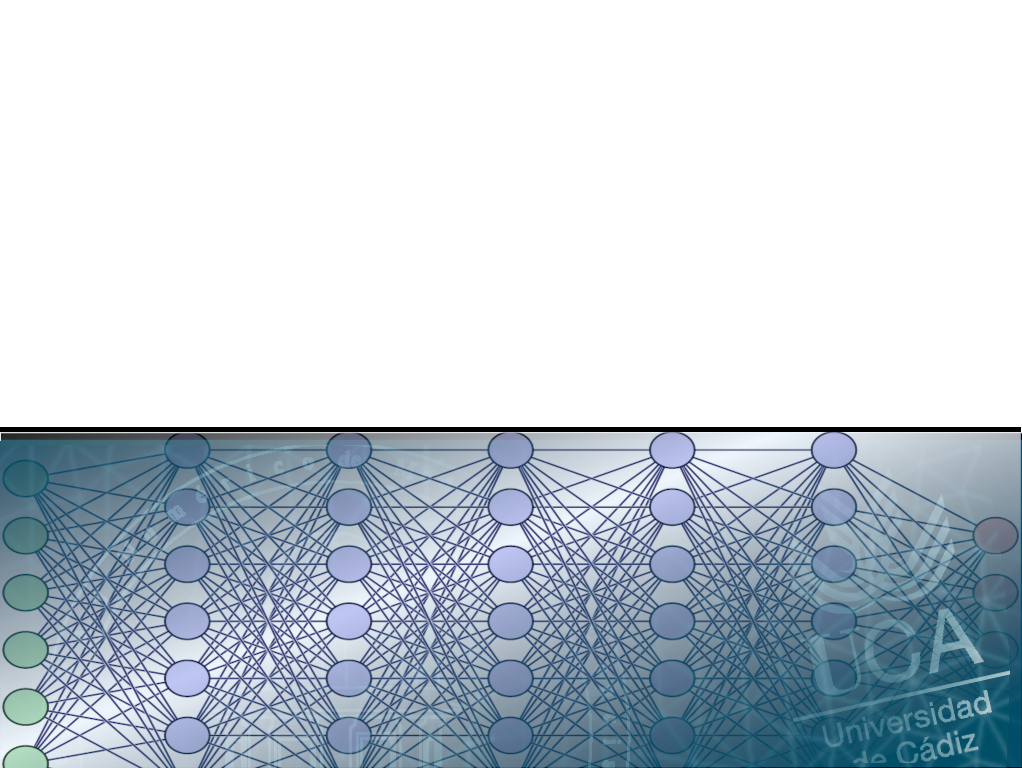
\includegraphics[width=\paperwidth,height=\paperheight]{frontpage_bg}}
\setbeamertemplate{footline}[default]
% <<<-------


% Write custom titlepage ------->>>
%\begin{frame}
%  \titlepage
%  \vspace{5cm}
%\end{frame}

% Set the background for the rest of the slides.
\setbeamertemplate{background}{}
 % {
\includegraphics[width=\paperwidth,height=\paperheight]{slide_bg}}


% Write all of the slides..........

% \begin{frame}{Outline}
%   \tableofcontents
% \end{frame}

% Start inserting infoline at the end
\setbeamertemplate{footline}[PHDtheme]
% <<<-------

%\newcommand{\imgdir}{Undefined, use renewcommand!}

%============================================================================
\section{Migración de neuroblastos en el cerebro adulto}
%============================================================================

%=====================================================================
\begin{frame}{¿Qué queremos modelar?}
%---------------------------------------------------------------------
\only<1>{
  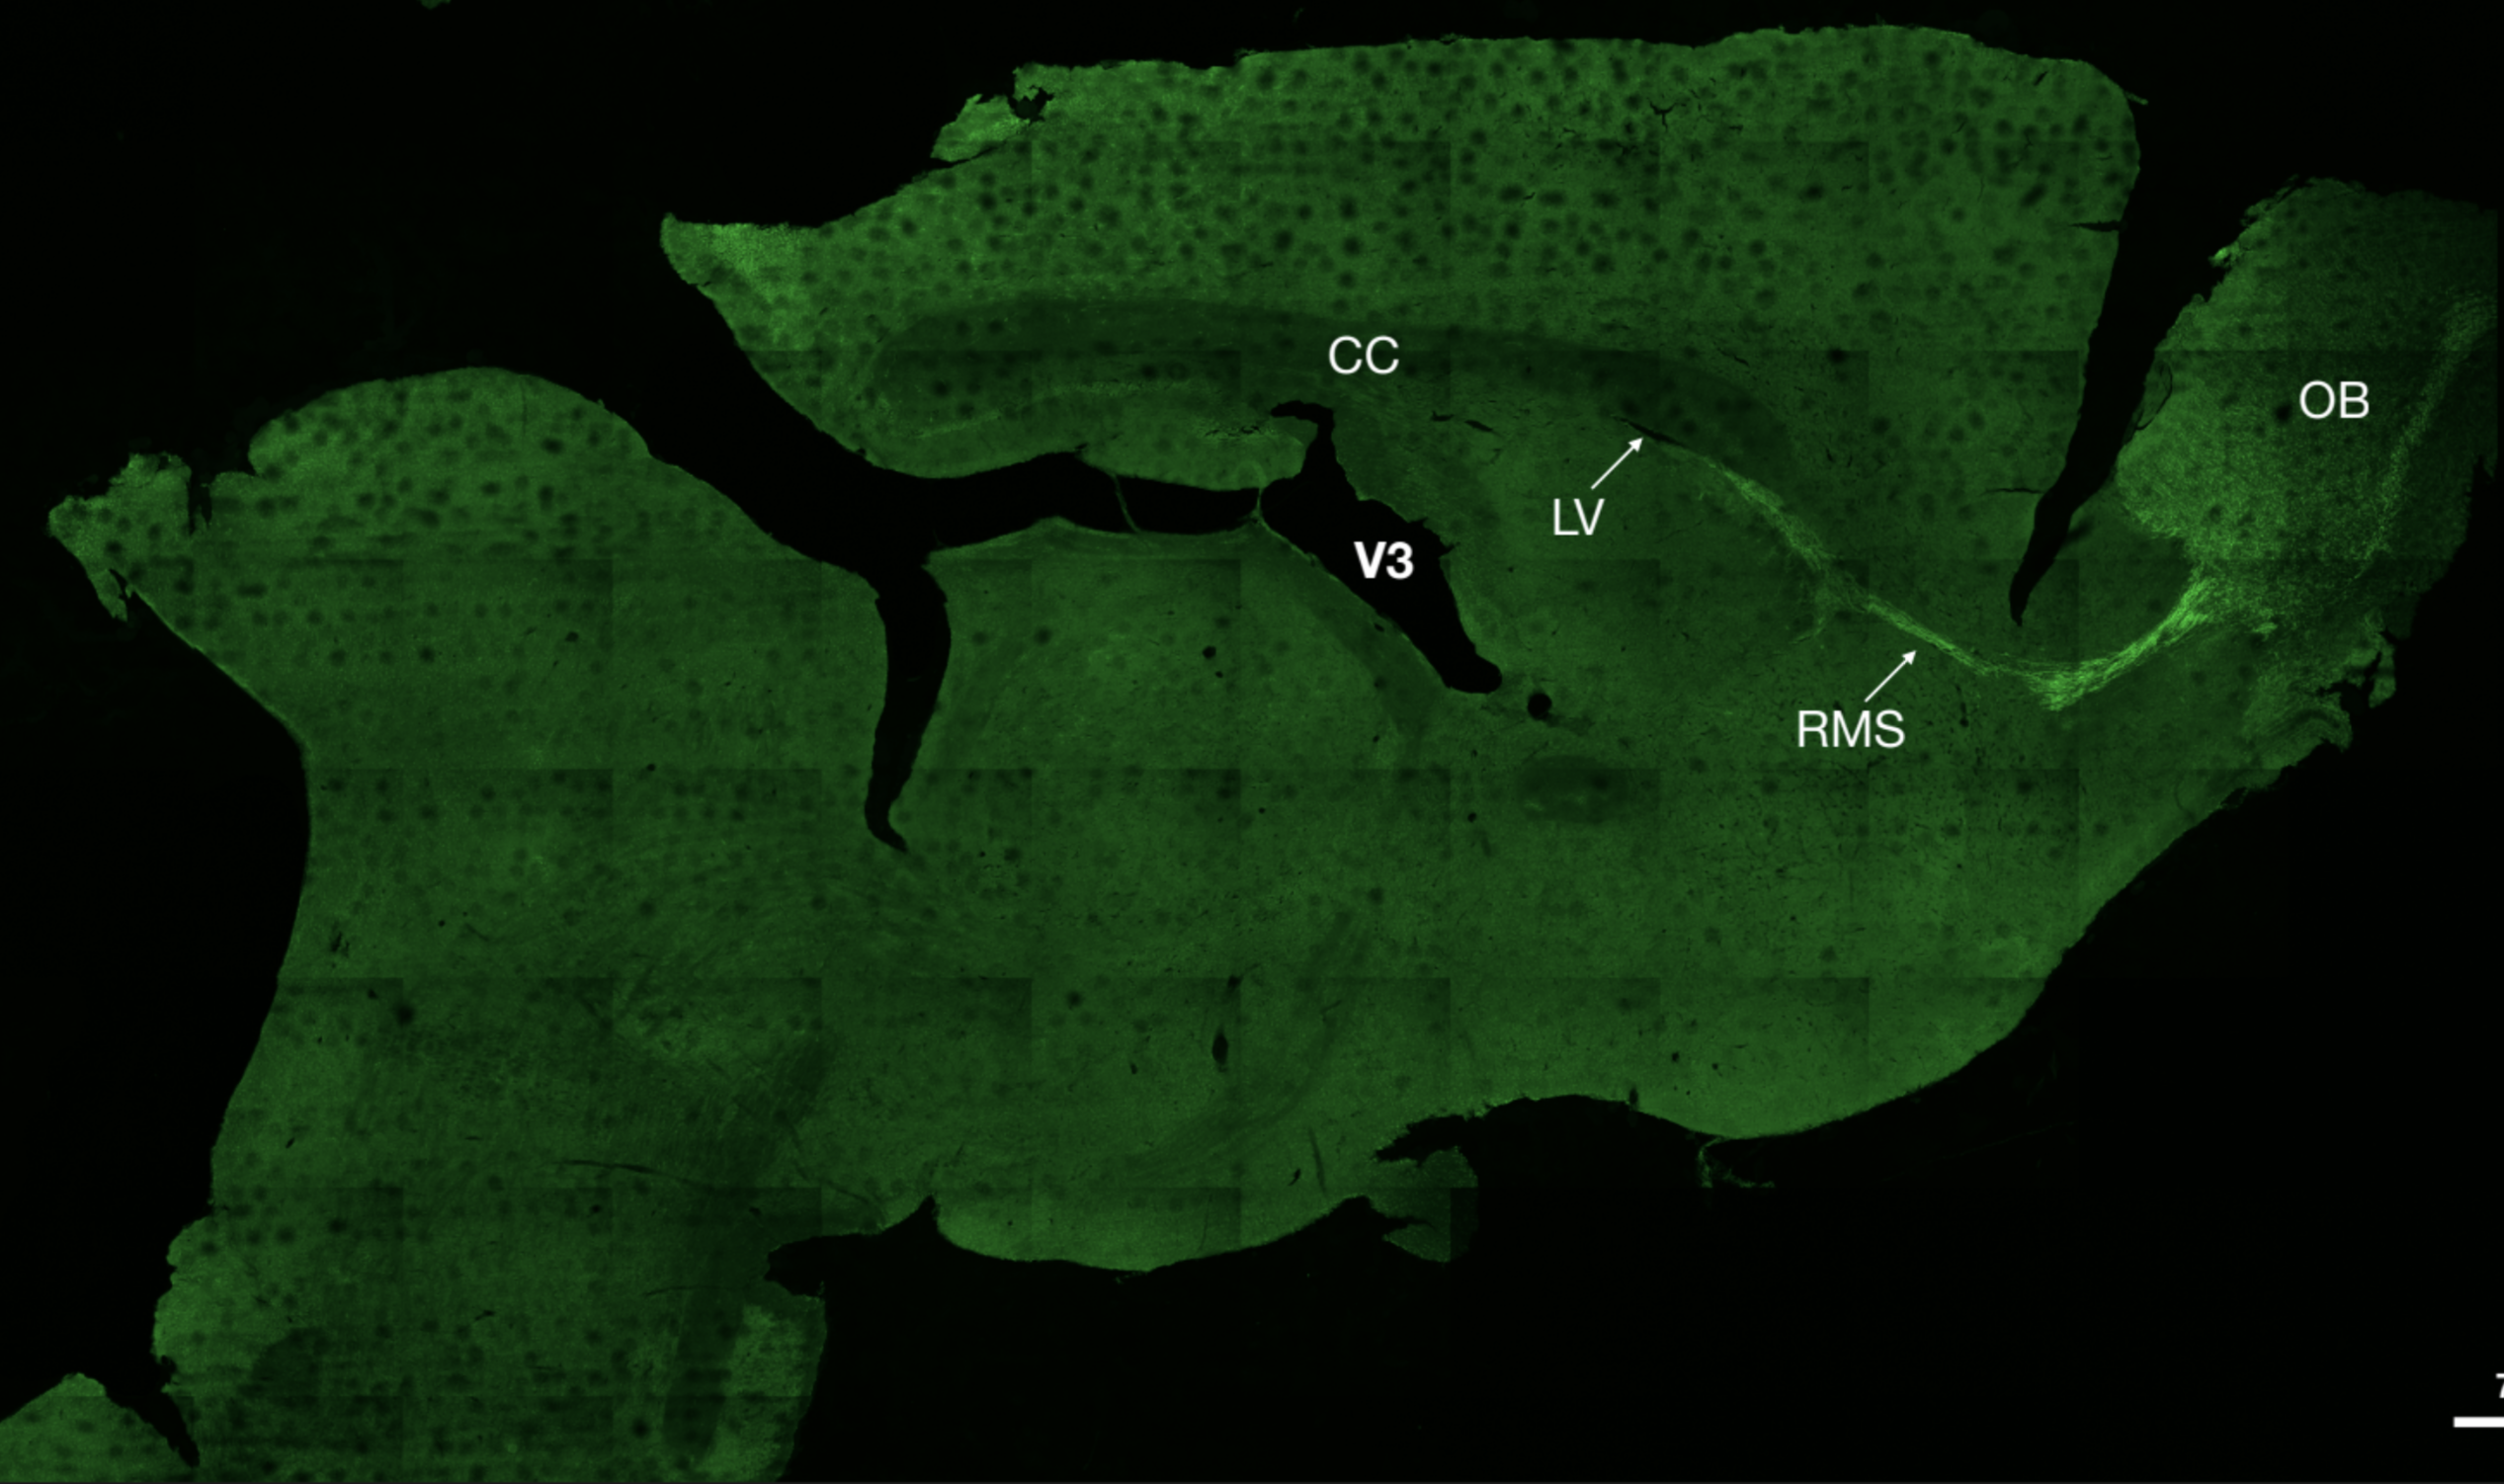
\includegraphics[width=0.95\linewidth]{cerebro-completo}}
  \only<2->{
  \includegraphics[width=0.95\linewidth]{via-rostral}}
\end{frame}

\begin{frame}{Primer objetivo: recuento de neuroblastos}
  \only<1>{
  	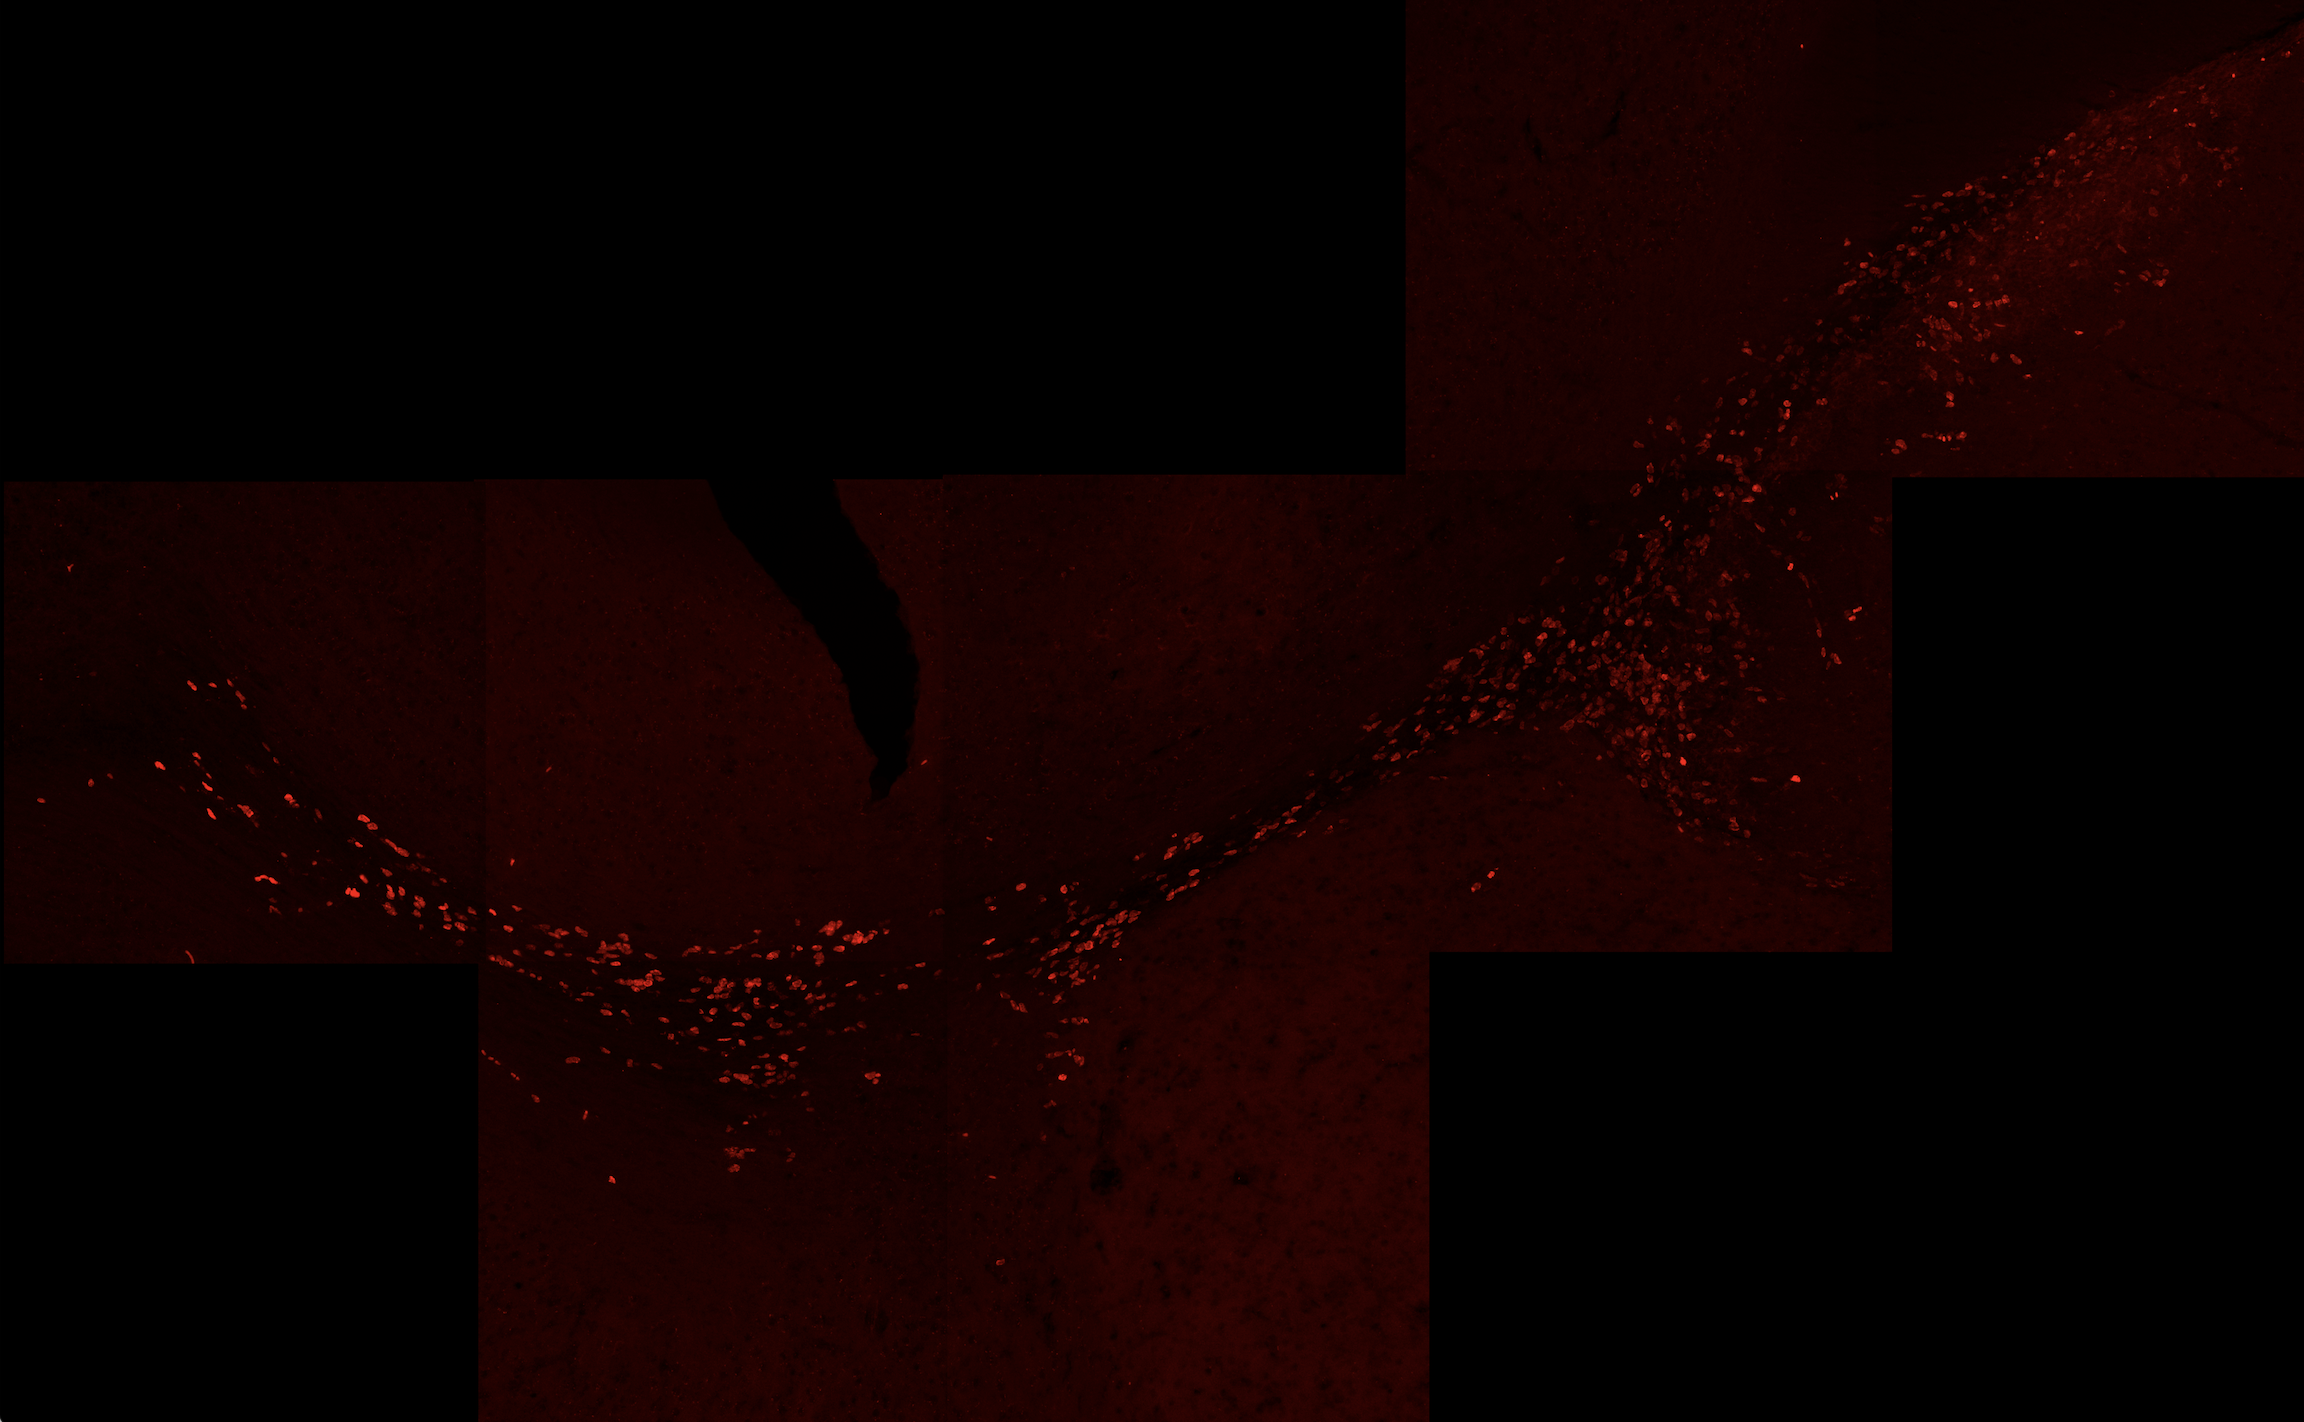
\includegraphics[width=0.95\linewidth]{via-roja}}
  \only<2->{
  	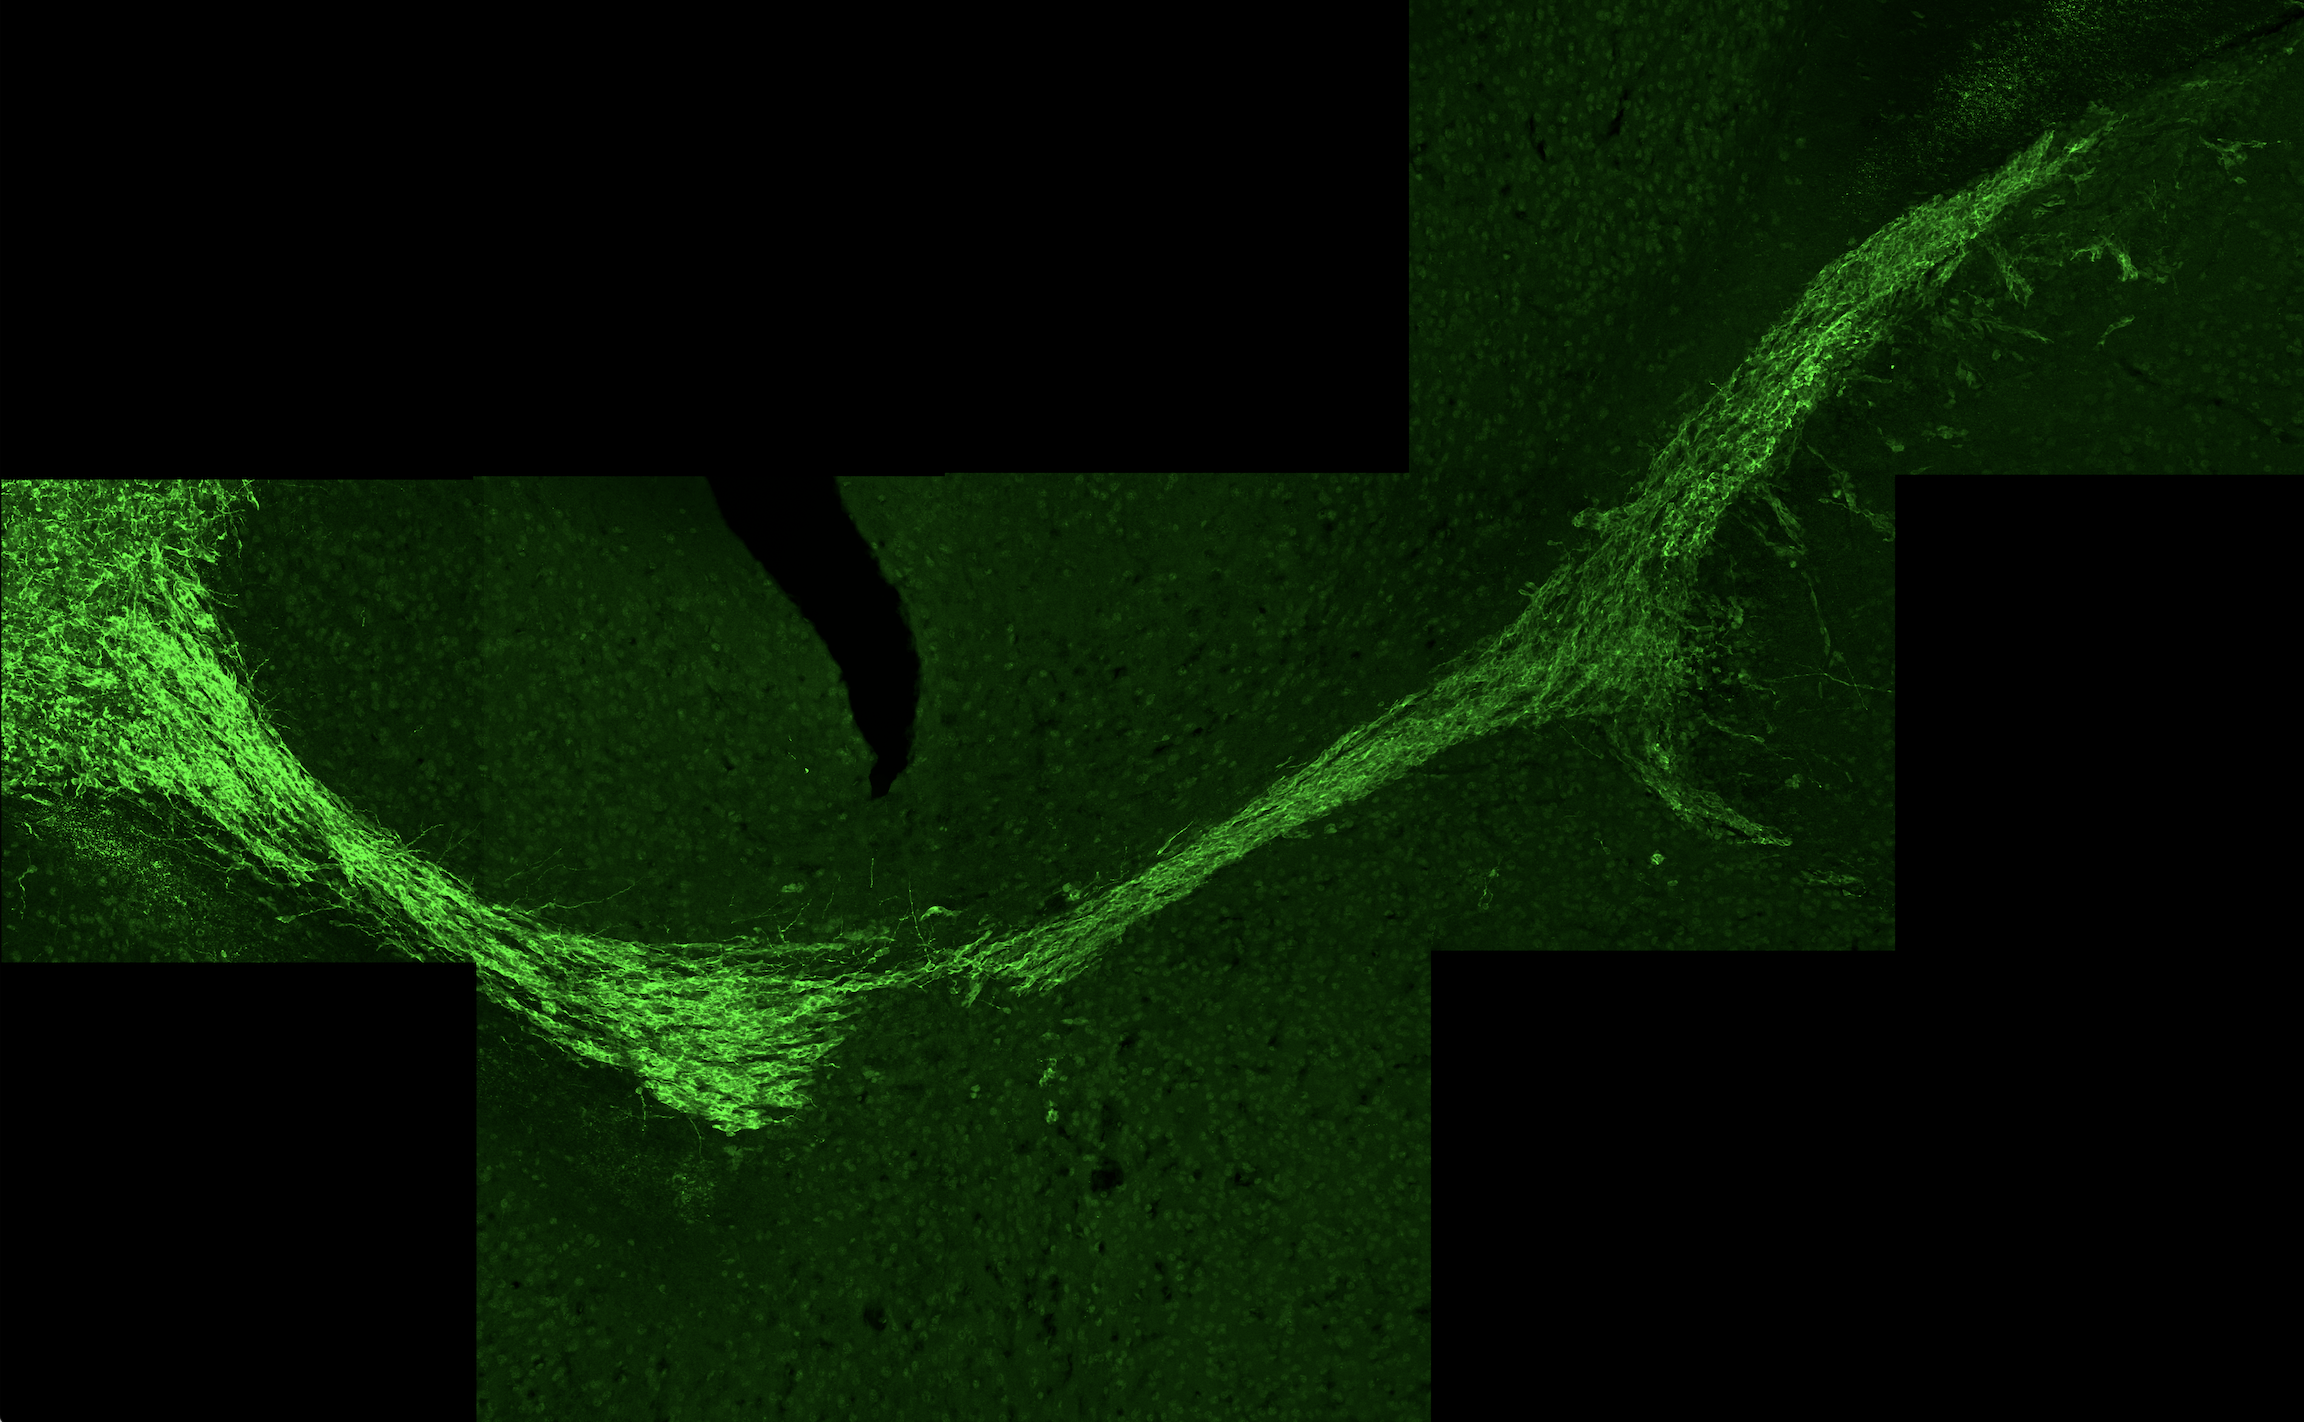
\includegraphics[width=0.95\linewidth]{via-verde}}
\end{frame}

\begin{frame}{Segundo objetivo: modelización y ajuste de parámetros}
	\begin{equation}
	\label{eq:neuroblast}
	\tau u_t + \X\, \nabla \cdot(u\nabla \O) + \alpha\, u - \gamma\, u \,1_{\NZdomain} 
	= \beta\, 1_{\SVZdomain}  
	\qquad\text{in}\enspace\Omega\times [0,T],
	\end{equation}
	\vspace{3mm}
	\begin{equation}
	\label{source}
	f_{\O}(x,y) = f_{\O}(\SO; x,y) 
	=  e^{((x-x_O)^2 + (y-y_O)^2)/\SO^2}.
	\end{equation}
	\vspace{3mm}
	\begin{equation} 
	\label{ob}
	\left\{ \begin{aligned} \Olf-\nabla\cdot (\mu_\CCdomain\,\nabla \Olf) &= f_{\O}  \quad  \text{ in } \Omega, \\
	\Olf &= f_{\O}  \quad \text{ on } \partial\Omega.
	\end{aligned}
	\right.
	\end{equation}
\end{frame}

\begin{frame}{Cerebro virtual}
	Malla
	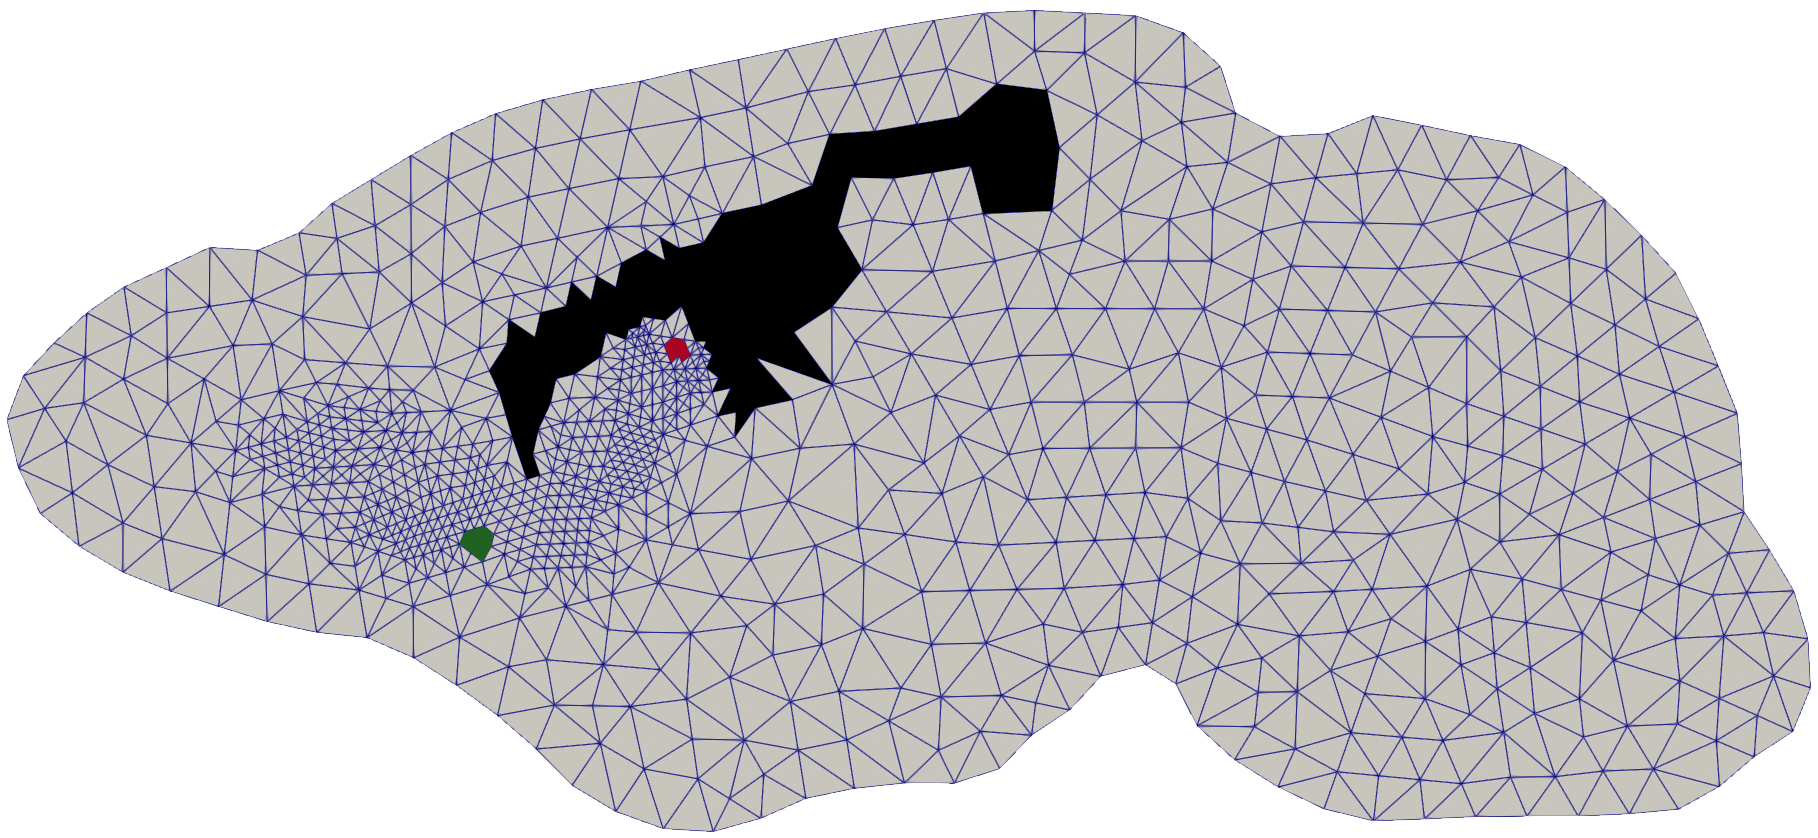
\includegraphics[width=0.95\linewidth]{brain-mesh.png}
\end{frame}

\begin{frame}{Modelización de la atracción}
Gradiente del bulbo olfatorio: parámetro $\sigma$
 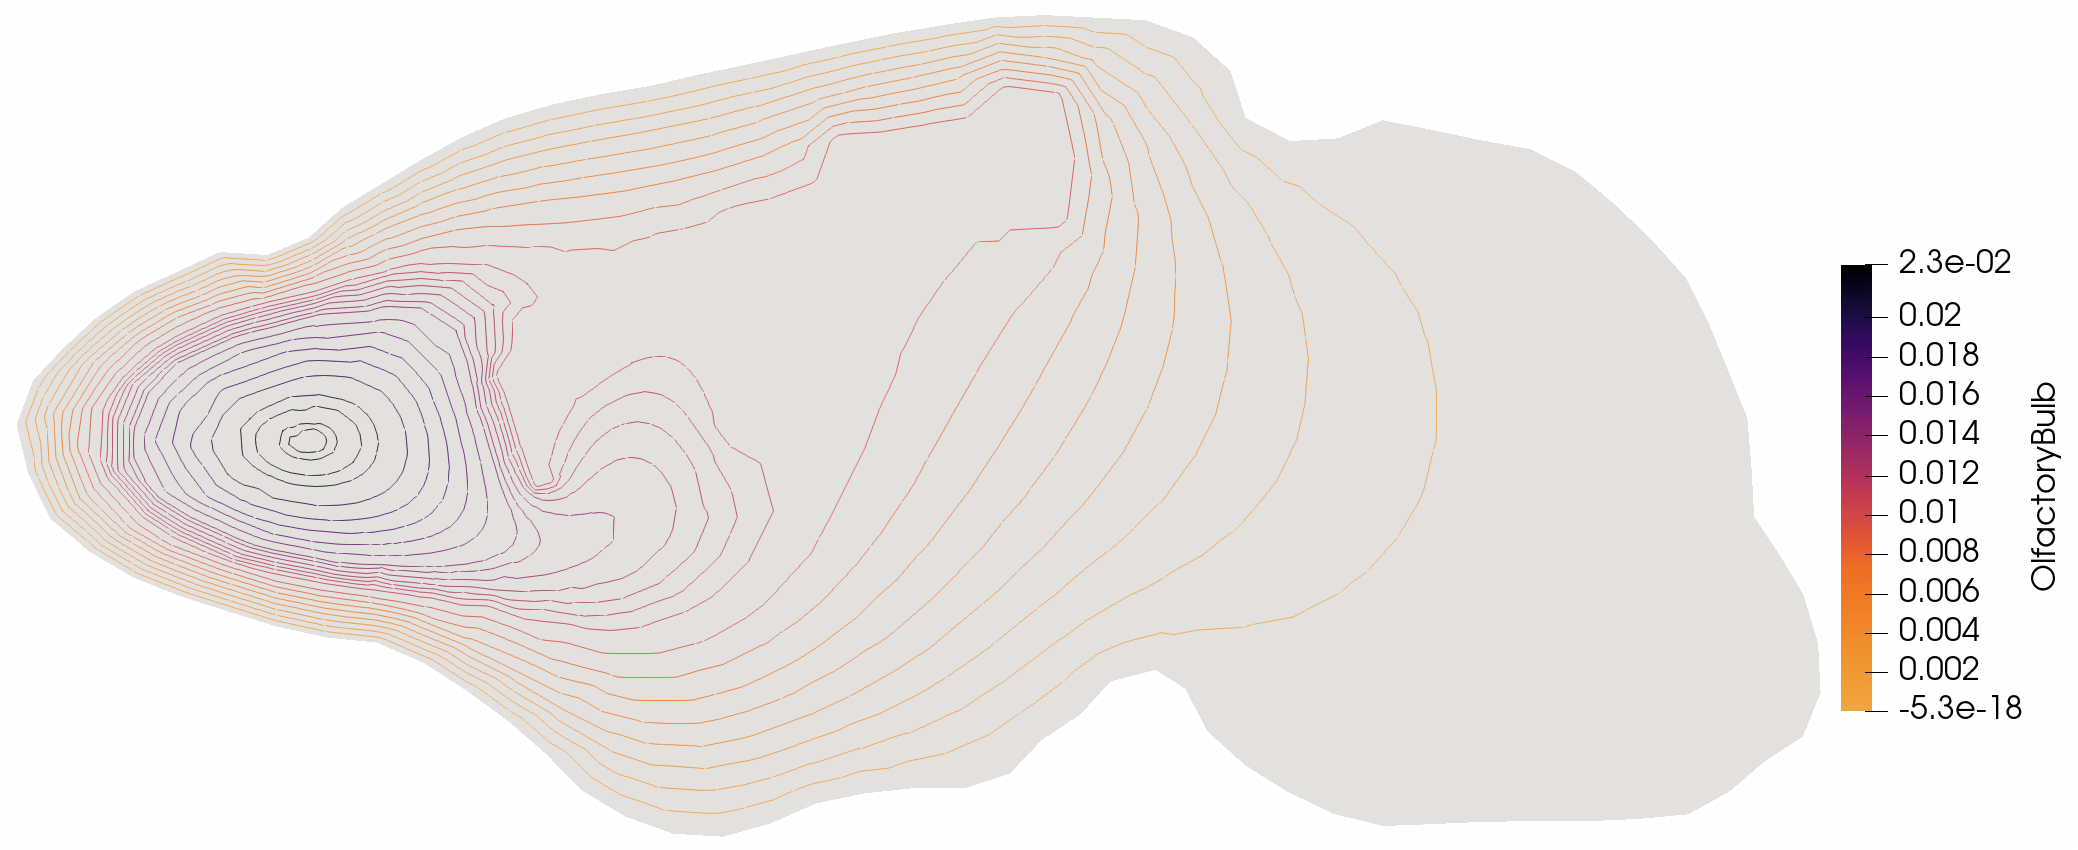
\includegraphics[width=0.95\linewidth]{ob.png}
\end{frame}
\begin{frame}{Modelización del movimiento}
	Vía rostral: parámetros $\alpha, \beta, \X, \gamma$
	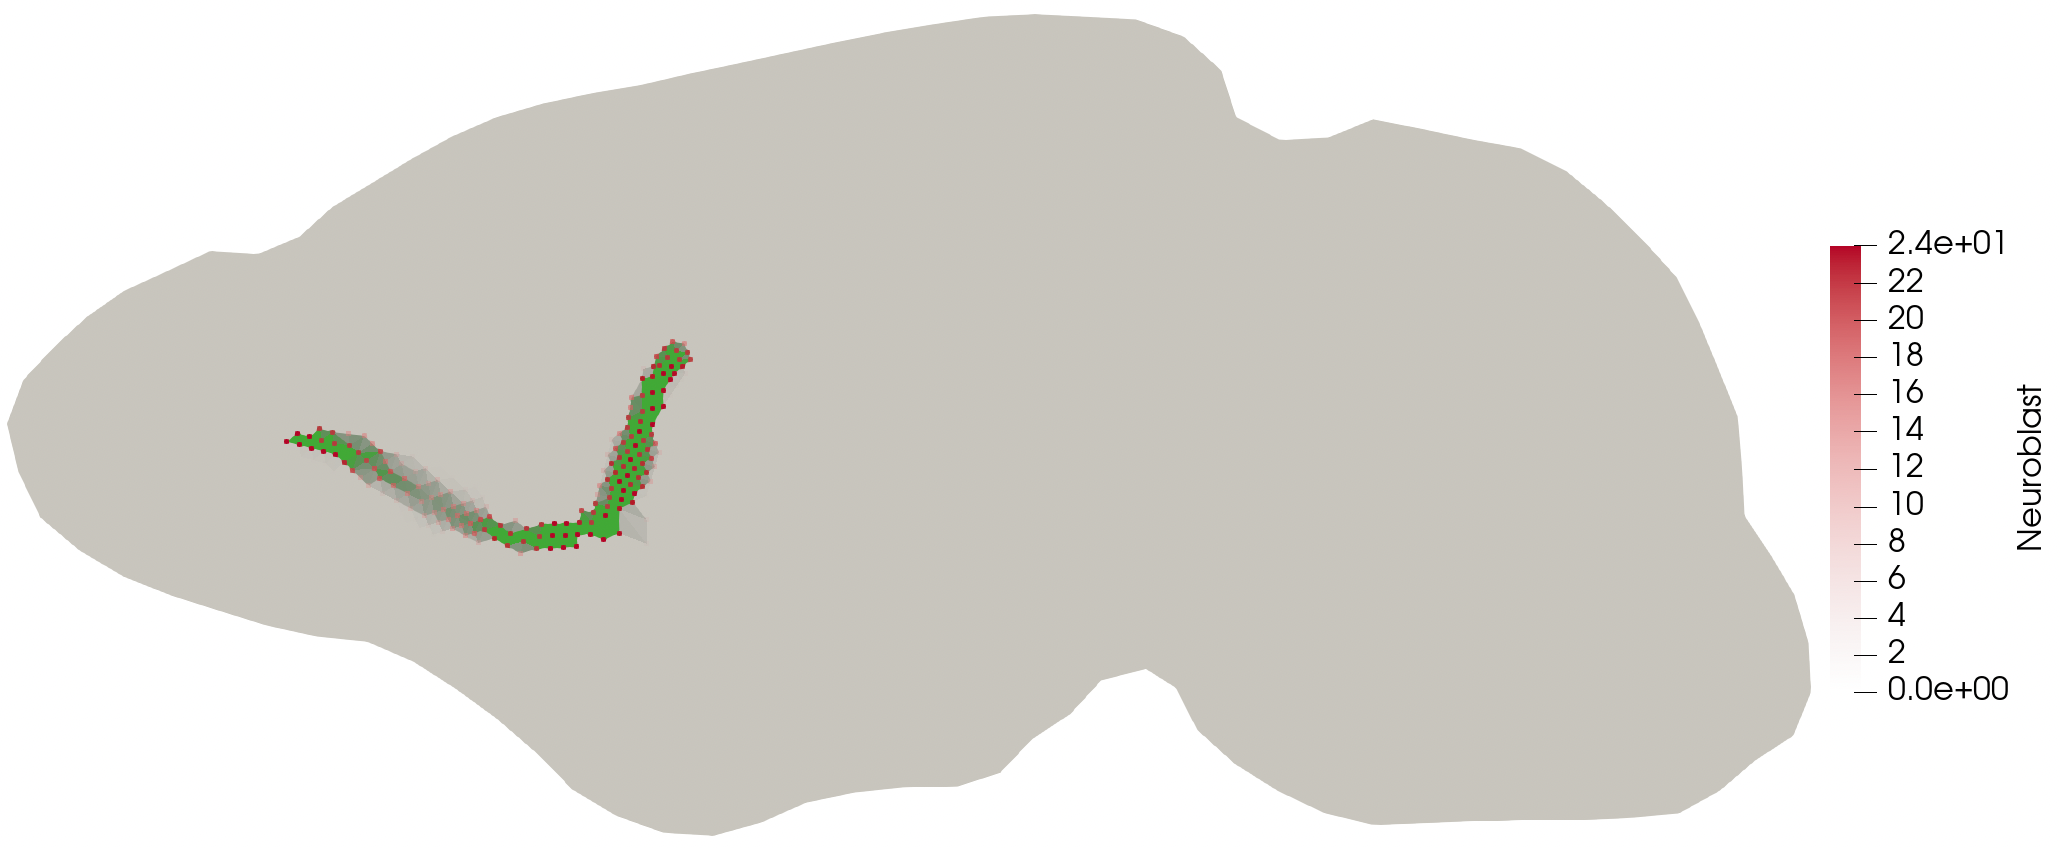
\includegraphics[width=0.95\linewidth]{steady-opt.png}
\end{frame}




%\include{dan1}
%
%% Beamer style >>>>>>>>>>>>>>>>>>>>>>>>>

\setbeamertemplate{enumerate item}[mycircle]

\setbeamertemplate{frametitle continuation}[from second][] % No automatic symbols I II II
%<<<<<<<<<<<<< beamer style

%\title{Redes Neuronales y otros Artefactos Matemáticos\vspace{-0.5em}}
%\author[J.R. Rodr\'{\i}guez Galv\'an]{\em\structure{Daniel Acosta Soba, Noelia Ortega Román, Álex Pérez Fernández, Rafa Rodríguez Galván}\vspace{-1.5em}}
%\date{\scriptsize{Facultad de Ciencias, Universidad de C\'adiz}\\[0.9em]\small Día Internacional de las Matemáticas («día {\Huge$\pi$}»), 2023}

% XeLaTeX font choosing
% \usepackage{fontspec}%{xltxtra} %fontspec}
% \setsansfont{Fontin Sans}
% \setsansfont{Lato}


\setcounter{tocdepth}{1}
\newcommand{\Olf}{\mathcal{O}}
\newcommand{\SVZdomain}{\text{\it SVZ}}
\newcommand{\NZdomain}{\text{\it NZ}}
\newcommand{\CCdomain}{{\text{\it CC}}}
\newcommand{\CCexp}{\mu_{CC}}
\newcommand{\tCCexp}{\tilde{\mu}_{CC}}
\def\SO{\sigma}
\def\X{\chi}
\def\D{\mathscr{D}}
\def\T{\mathcal{T}}
\def\E{\mathcal{E}}
\def\S{\mathcal{S}}
\def\N{\mathbb{N}}
\def\P{\mathbb{P}}
\def\O{\mathcal{O}}

%
% Bibliography
%
%\usepackage{natbib}

% To list each bibliographic entry in a line
\setbeamertemplate{bibliography entry title}{}
\setbeamertemplate{bibliography entry location}{}
\setbeamertemplate{bibliography entry note}{}

% ... end of preamble.

\AtBeginSection{\frame{\sectionpage}}

\colorlet{inputcolor}{green!60!black}
\colorlet{hiddencolor}{blue!60!black}
\colorlet{outcolor}{red!60!black}

%======================================================================

%======================================================================

% Tikz style and beamer template ------->>>
\tikzstyle{every picture}+=[remember picture]
\tikzstyle{na} = [baseline=-.5ex]
\tikzstyle{phd} = [baseline=-.6ex,
  box/.style={rectangle, draw=PHDblueC, thick, fill=PHDblueA,
    align=center, rounded corners, minimum height=1.6em},
  boxB/.style={rectangle, draw=PHDredA, thick, fill=PHDblueA,
    align=center, rounded corners, minimum height=1.6em}]
\tikzstyle{phdB} = [baseline=-.7ex,
  box/.style={rectangle, draw=PHDblueC, thick, fill=PHDblueA,
    align=center, rounded corners, minimum height=1.6em},
  boxB/.style={rectangle, draw=PHDredA, thick, fill=PHDblueA,
    align=center, rounded corners, minimum height=1.6em}]
\tikzstyle{myarrow} = [->,>=latex, PHDredA, shorten >=4pt,
  opacity=.6, line width=0.6mm]
\tikzstyle{myarrow2} = [->,>=latex, PHDblueC, shorten >=4pt, opacity=.2, line width=0.4mm]
\tikzstyle{myarrow3} = [
     opacity=.7,
%    >=triangle 60,              % Nice arrows; your taste may be different
    node distance=6mm and 60mm, % Global setup of box spacing
    every join/.style={norm},   % Default linetype for connecting
                                % boxes
    line width=0.6mm,
    PHDredA,
    ->
    ]
\setbeamertemplate{background}
 {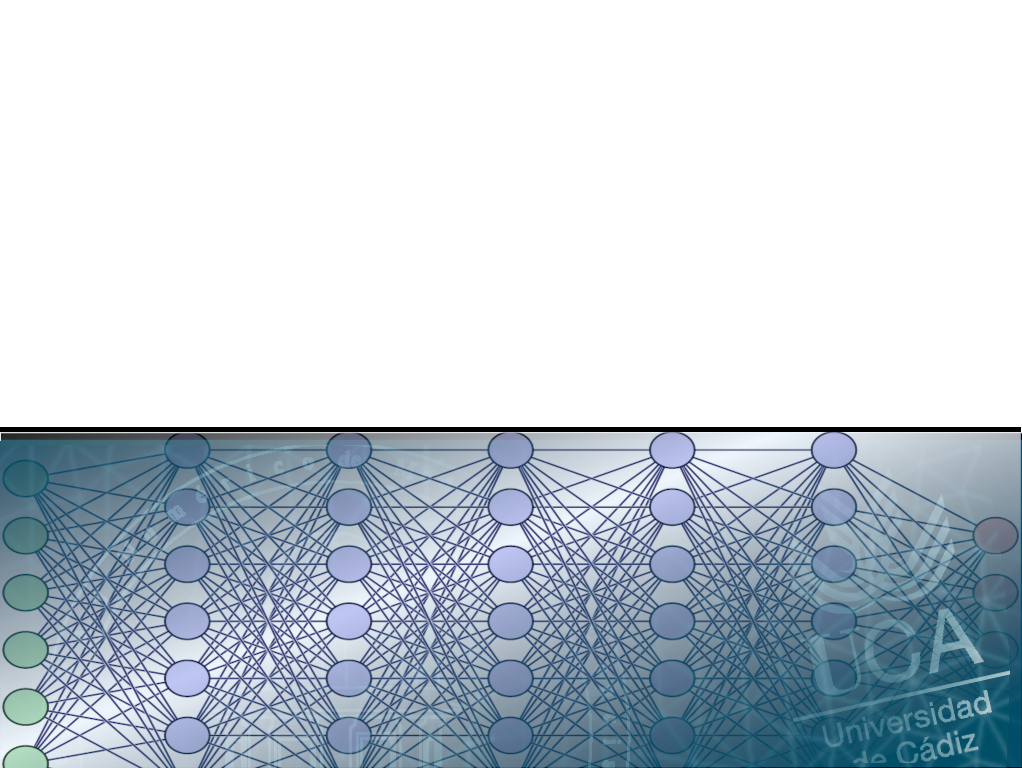
\includegraphics[width=\paperwidth,height=\paperheight]{frontpage_bg}}
\setbeamertemplate{footline}[default]
% <<<-------


% Write custom titlepage ------->>>
%\begin{frame}
%  \titlepage
%  \vspace{5cm}
%\end{frame}

% Set the background for the rest of the slides.
\setbeamertemplate{background}{}
 % {
\includegraphics[width=\paperwidth,height=\paperheight]{slide_bg}}


% Write all of the slides..........

% \begin{frame}{Outline}
%   \tableofcontents
% \end{frame}

% Start inserting infoline at the end
\setbeamertemplate{footline}[PHDtheme]
% <<<-------

%\newcommand{\imgdir}{Undefined, use renewcommand!}

%============================================================================
\section{Migración de neuroblastos en el cerebro adulto}
%============================================================================

%=====================================================================
\begin{frame}{¿Qué queremos modelar?}
%---------------------------------------------------------------------
\only<1>{
  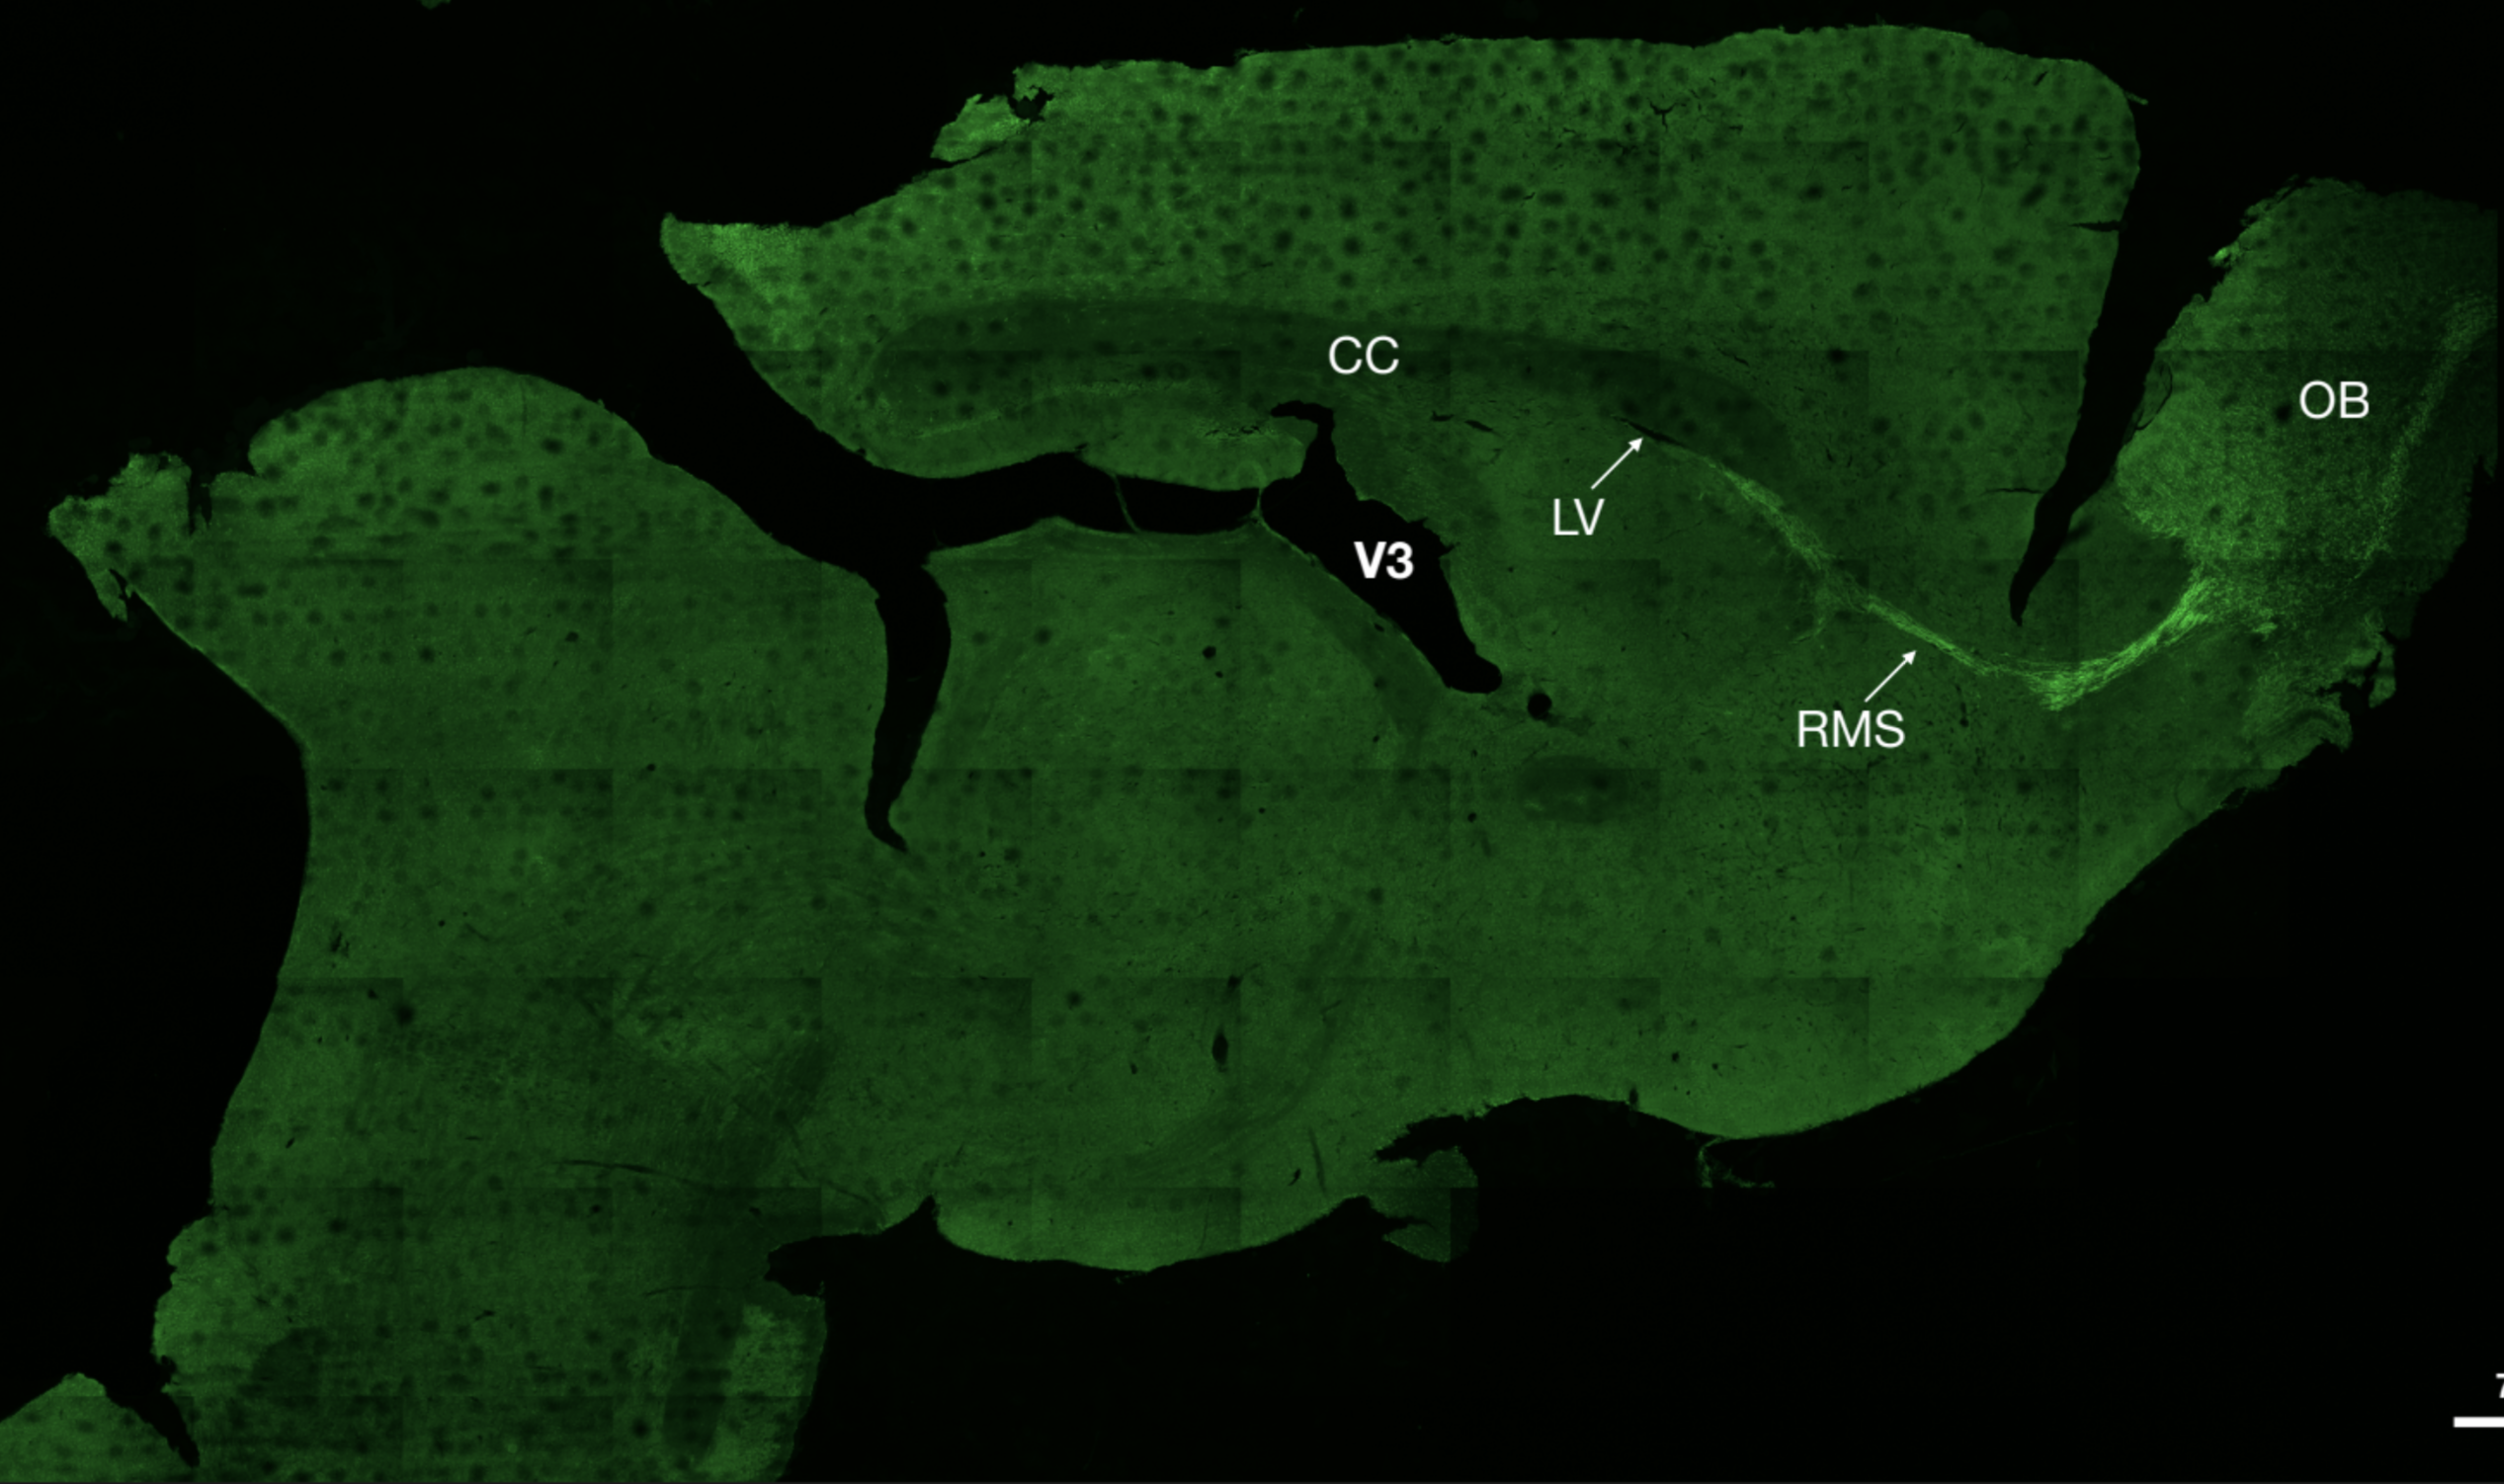
\includegraphics[width=0.95\linewidth]{cerebro-completo}}
  \only<2->{
  \includegraphics[width=0.95\linewidth]{via-rostral}}
\end{frame}

\begin{frame}{Primer objetivo: recuento de neuroblastos}
  \only<1>{
  	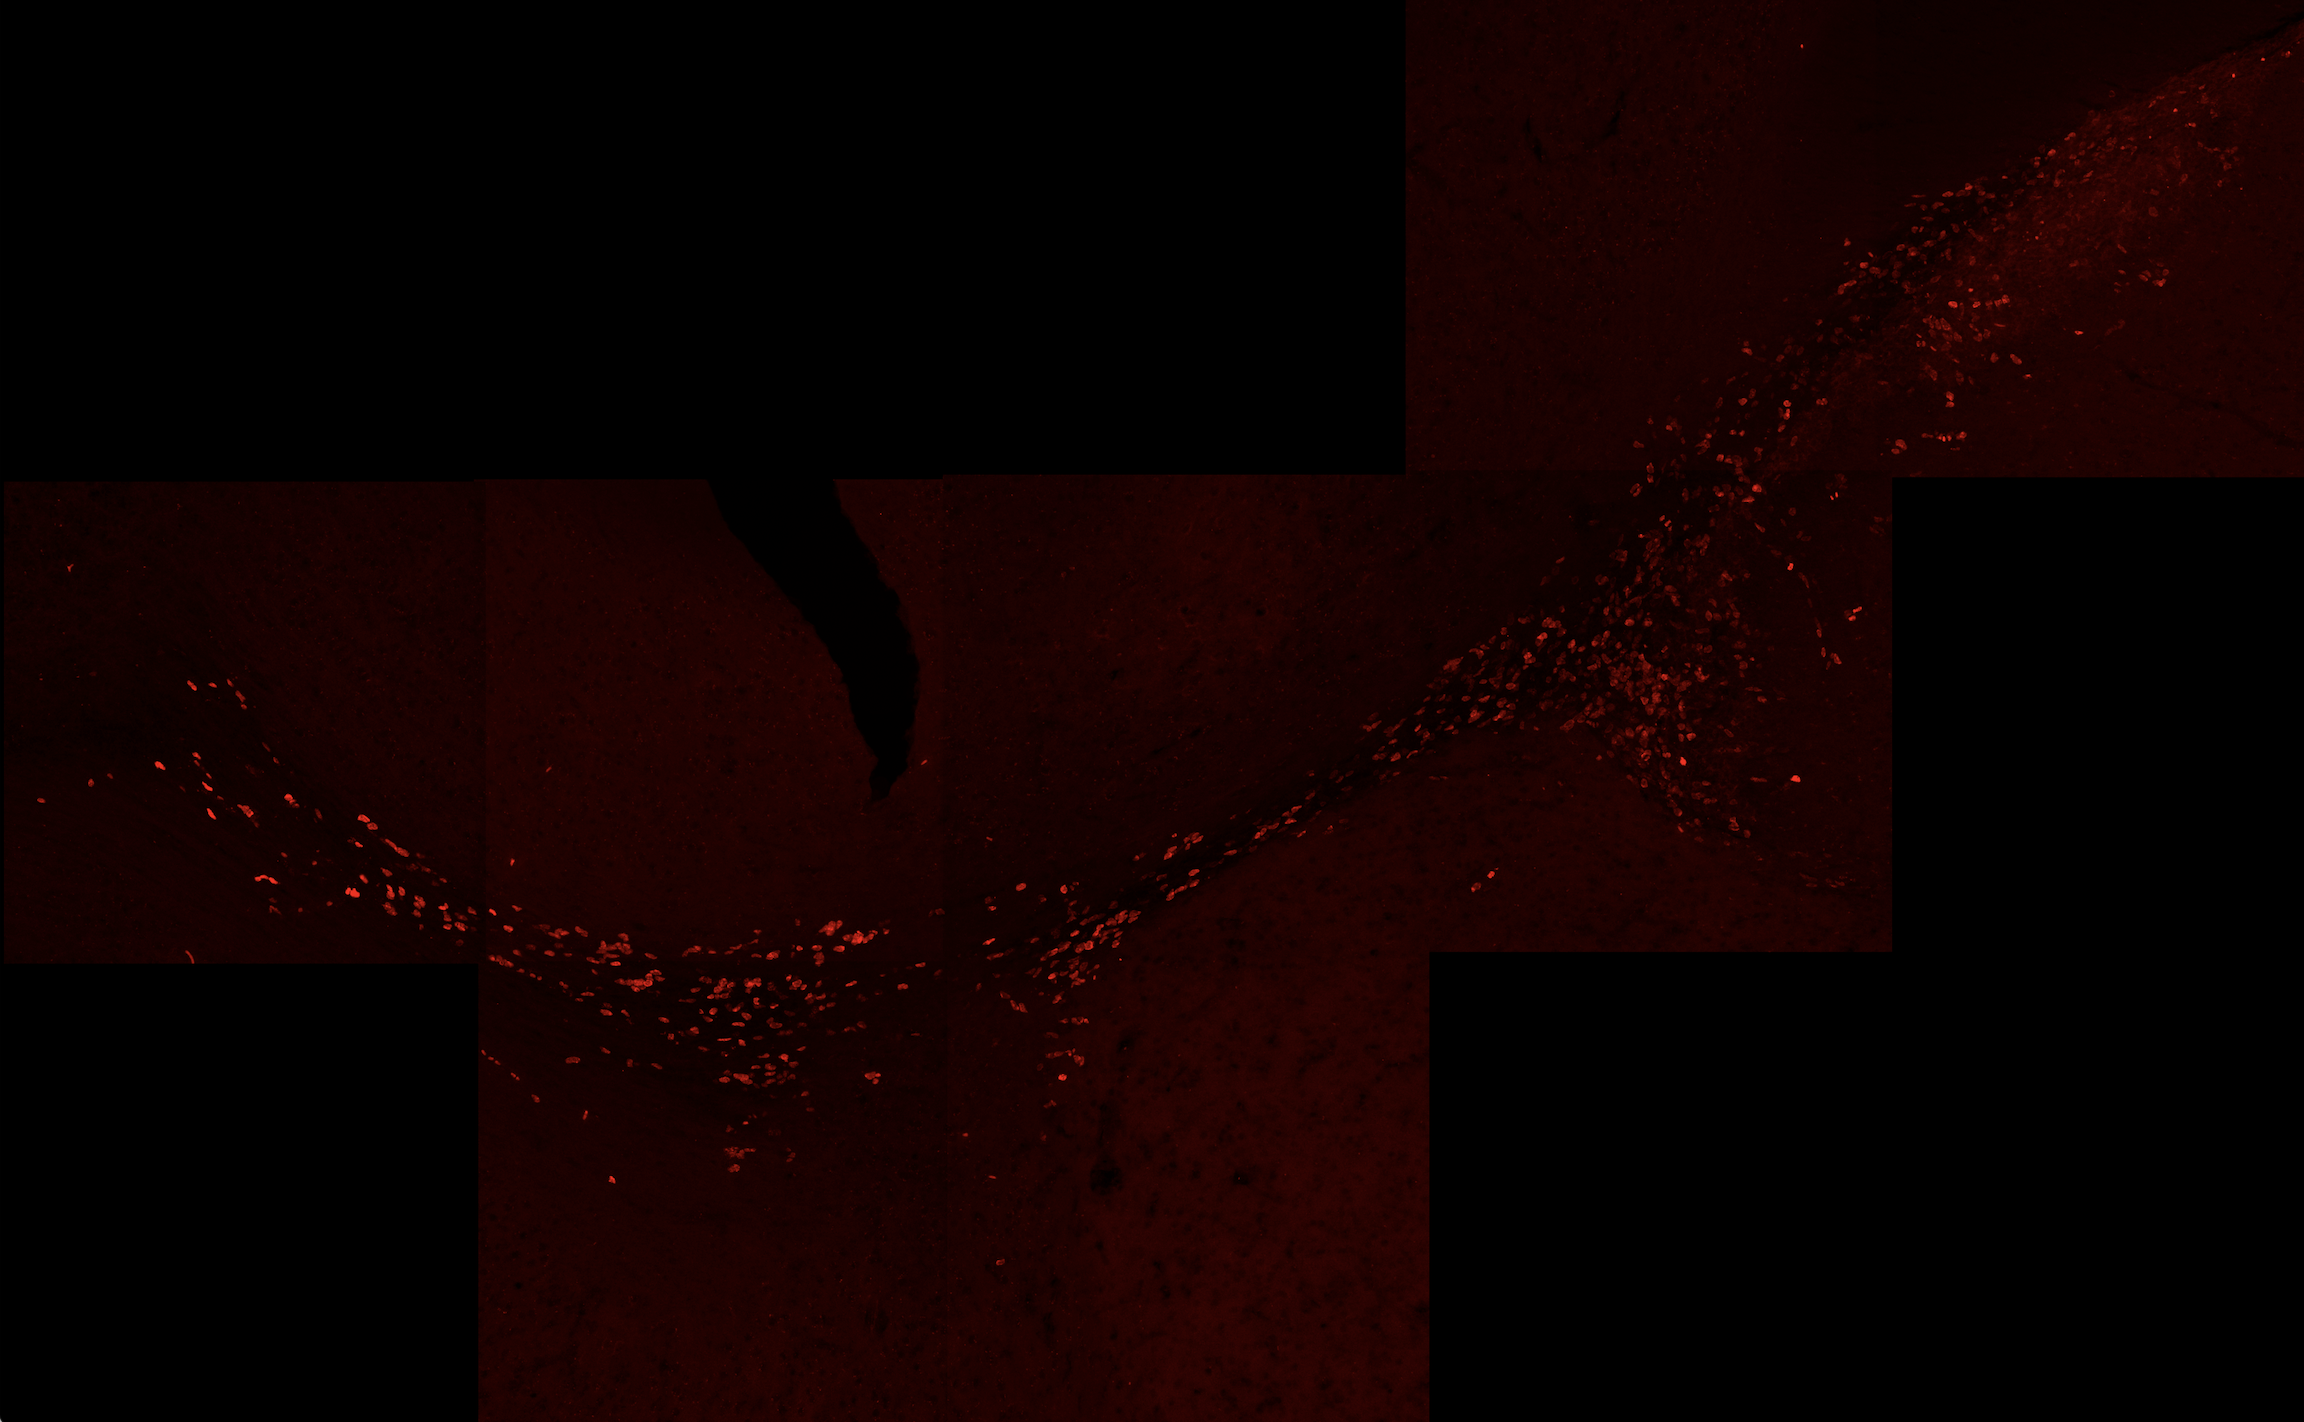
\includegraphics[width=0.95\linewidth]{via-roja}}
  \only<2->{
  	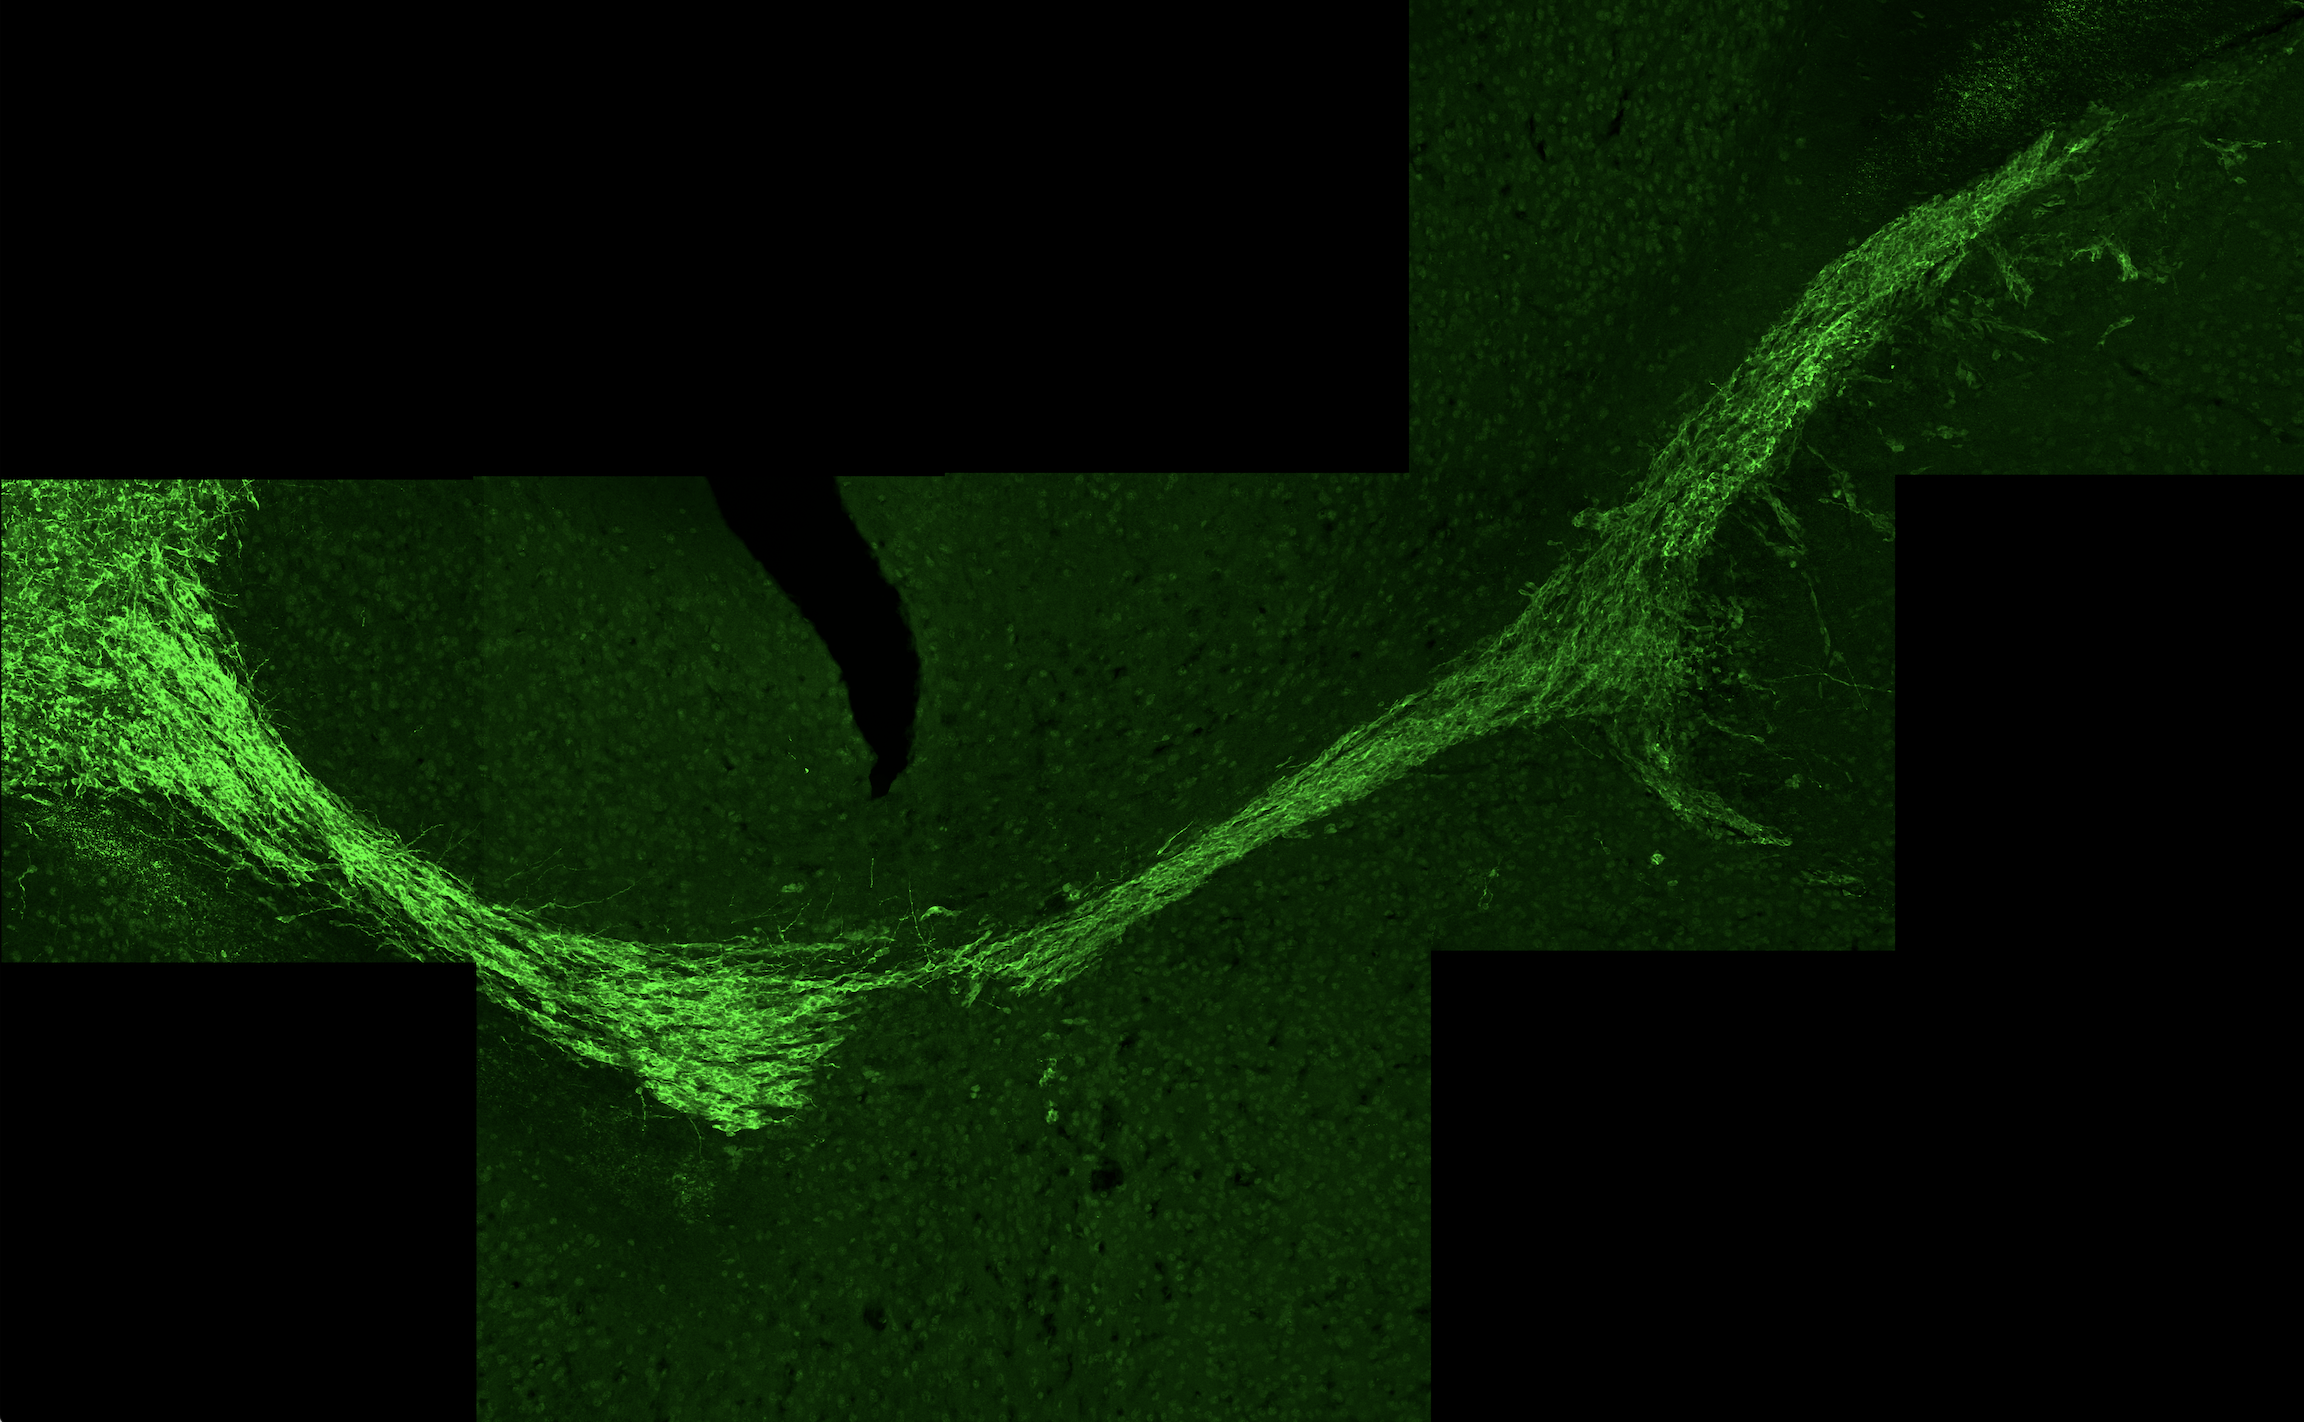
\includegraphics[width=0.95\linewidth]{via-verde}}
\end{frame}

\begin{frame}{Segundo objetivo: modelización y ajuste de parámetros}
	\begin{equation}
	\label{eq:neuroblast}
	\tau u_t + \X\, \nabla \cdot(u\nabla \O) + \alpha\, u - \gamma\, u \,1_{\NZdomain} 
	= \beta\, 1_{\SVZdomain}  
	\qquad\text{in}\enspace\Omega\times [0,T],
	\end{equation}
	\vspace{3mm}
	\begin{equation}
	\label{source}
	f_{\O}(x,y) = f_{\O}(\SO; x,y) 
	=  e^{((x-x_O)^2 + (y-y_O)^2)/\SO^2}.
	\end{equation}
	\vspace{3mm}
	\begin{equation} 
	\label{ob}
	\left\{ \begin{aligned} \Olf-\nabla\cdot (\mu_\CCdomain\,\nabla \Olf) &= f_{\O}  \quad  \text{ in } \Omega, \\
	\Olf &= f_{\O}  \quad \text{ on } \partial\Omega.
	\end{aligned}
	\right.
	\end{equation}
\end{frame}

\begin{frame}{Cerebro virtual}
	Malla
	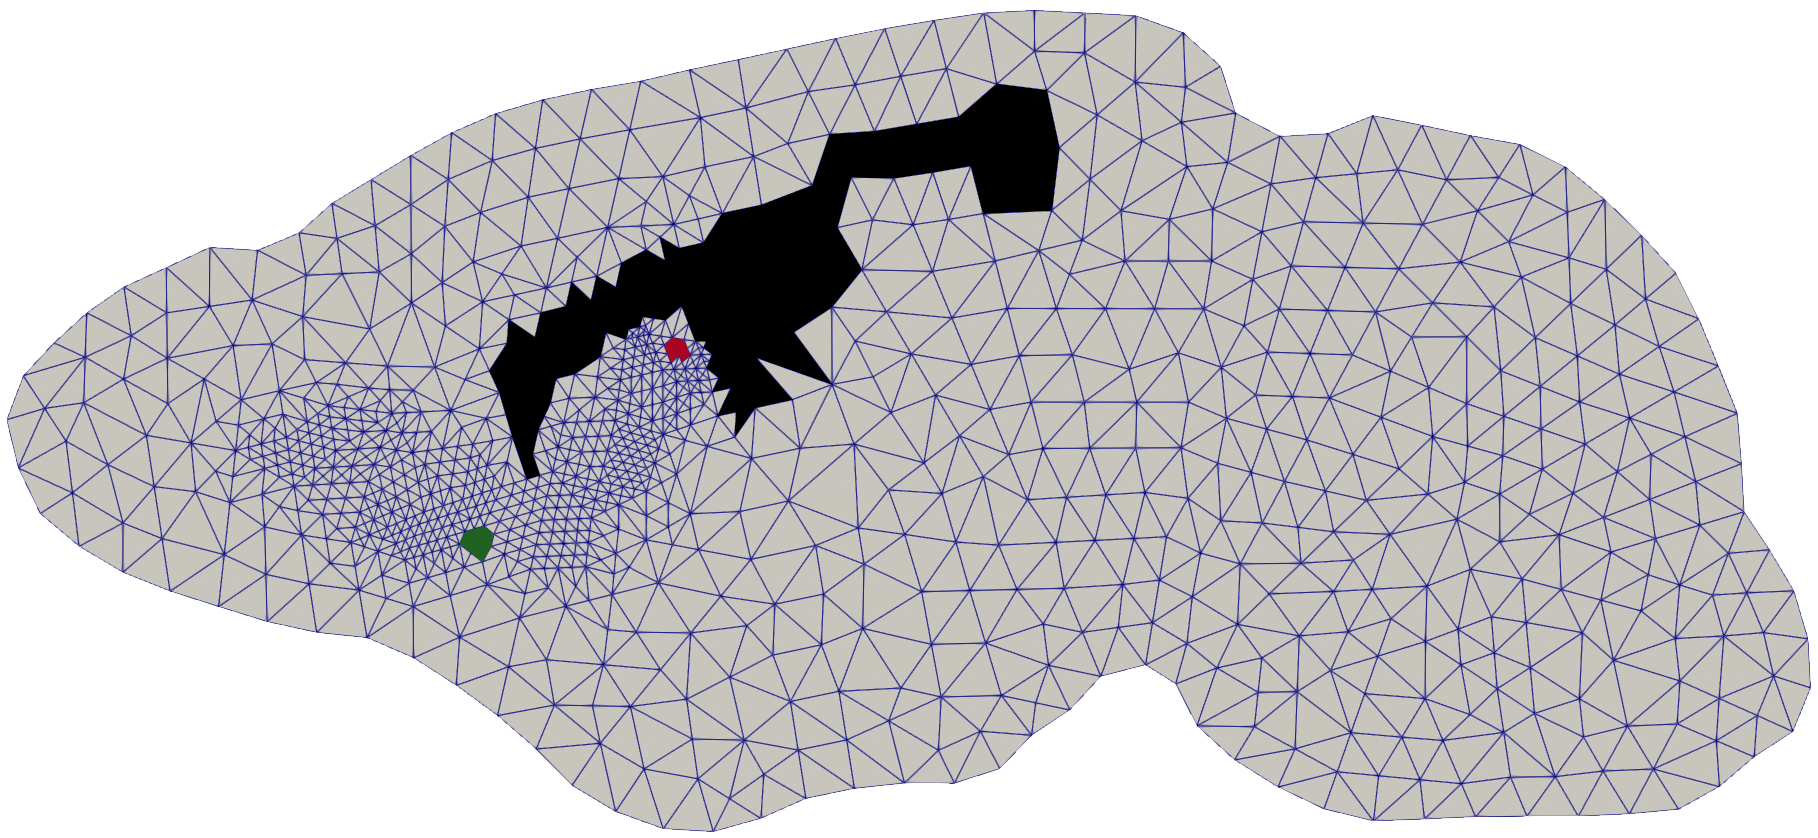
\includegraphics[width=0.95\linewidth]{brain-mesh.png}
\end{frame}

\begin{frame}{Modelización de la atracción}
Gradiente del bulbo olfatorio: parámetro $\sigma$
 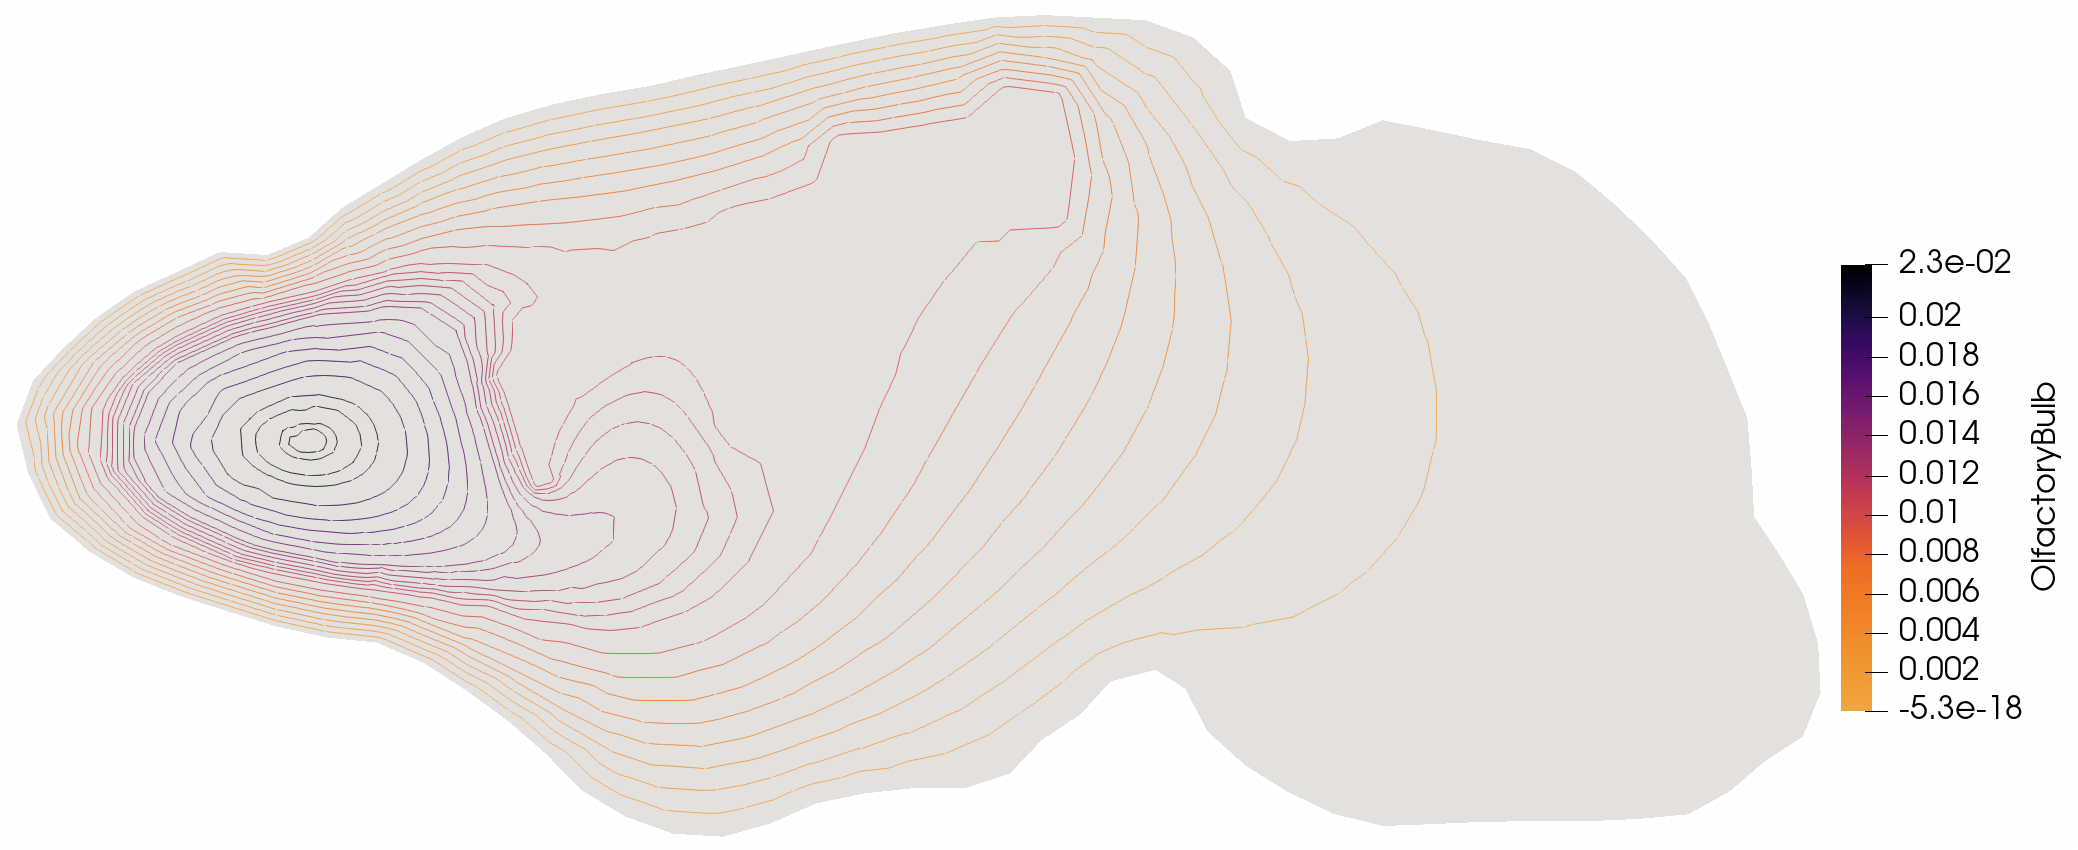
\includegraphics[width=0.95\linewidth]{ob.png}
\end{frame}
\begin{frame}{Modelización del movimiento}
	Vía rostral: parámetros $\alpha, \beta, \X, \gamma$
	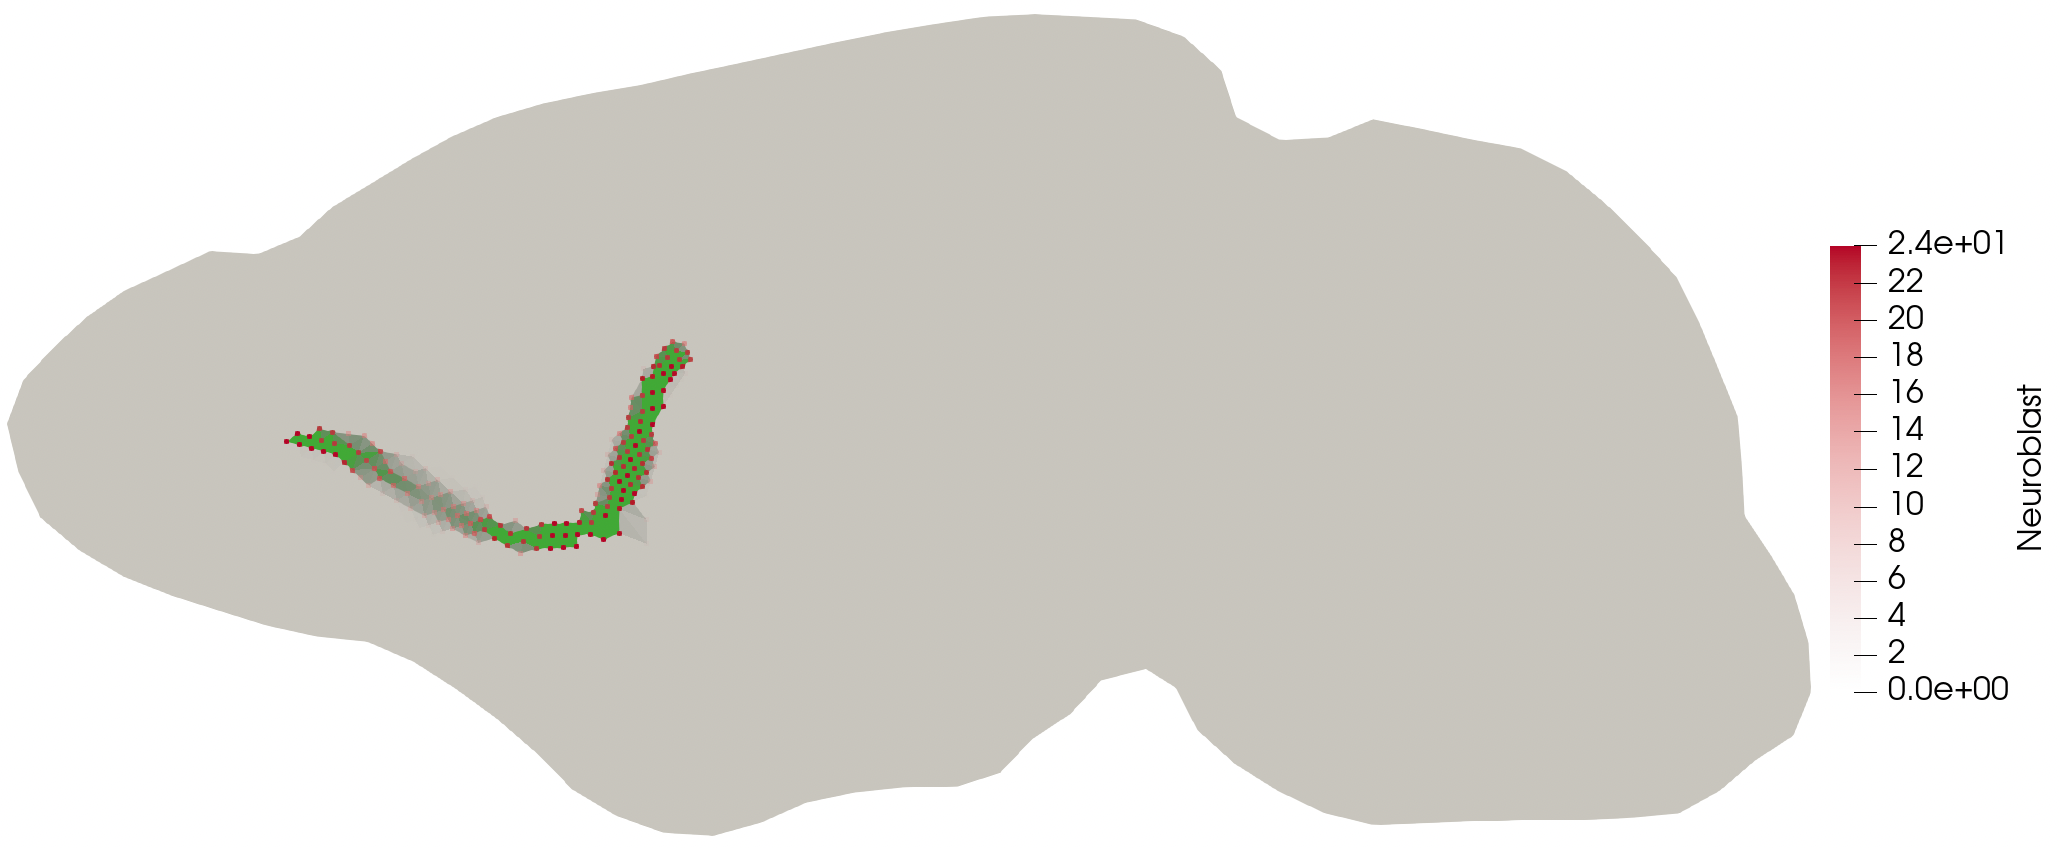
\includegraphics[width=0.95\linewidth]{steady-opt.png}
\end{frame}




%\include{dan1}
%
%% Beamer style >>>>>>>>>>>>>>>>>>>>>>>>>

\setbeamertemplate{enumerate item}[mycircle]

\setbeamertemplate{frametitle continuation}[from second][] % No automatic symbols I II II
%<<<<<<<<<<<<< beamer style

%\title{Redes Neuronales y otros Artefactos Matemáticos\vspace{-0.5em}}
%\author[J.R. Rodr\'{\i}guez Galv\'an]{\em\structure{Daniel Acosta Soba, Noelia Ortega Román, Álex Pérez Fernández, Rafa Rodríguez Galván}\vspace{-1.5em}}
%\date{\scriptsize{Facultad de Ciencias, Universidad de C\'adiz}\\[0.9em]\small Día Internacional de las Matemáticas («día {\Huge$\pi$}»), 2023}

% XeLaTeX font choosing
% \usepackage{fontspec}%{xltxtra} %fontspec}
% \setsansfont{Fontin Sans}
% \setsansfont{Lato}


\setcounter{tocdepth}{1}
\newcommand{\Olf}{\mathcal{O}}
\newcommand{\SVZdomain}{\text{\it SVZ}}
\newcommand{\NZdomain}{\text{\it NZ}}
\newcommand{\CCdomain}{{\text{\it CC}}}
\newcommand{\CCexp}{\mu_{CC}}
\newcommand{\tCCexp}{\tilde{\mu}_{CC}}
\def\SO{\sigma}
\def\X{\chi}
\def\D{\mathscr{D}}
\def\T{\mathcal{T}}
\def\E{\mathcal{E}}
\def\S{\mathcal{S}}
\def\N{\mathbb{N}}
\def\P{\mathbb{P}}
\def\O{\mathcal{O}}

%
% Bibliography
%
%\usepackage{natbib}

% To list each bibliographic entry in a line
\setbeamertemplate{bibliography entry title}{}
\setbeamertemplate{bibliography entry location}{}
\setbeamertemplate{bibliography entry note}{}

% ... end of preamble.

\AtBeginSection{\frame{\sectionpage}}

\colorlet{inputcolor}{green!60!black}
\colorlet{hiddencolor}{blue!60!black}
\colorlet{outcolor}{red!60!black}

%======================================================================

%======================================================================

% Tikz style and beamer template ------->>>
\tikzstyle{every picture}+=[remember picture]
\tikzstyle{na} = [baseline=-.5ex]
\tikzstyle{phd} = [baseline=-.6ex,
  box/.style={rectangle, draw=PHDblueC, thick, fill=PHDblueA,
    align=center, rounded corners, minimum height=1.6em},
  boxB/.style={rectangle, draw=PHDredA, thick, fill=PHDblueA,
    align=center, rounded corners, minimum height=1.6em}]
\tikzstyle{phdB} = [baseline=-.7ex,
  box/.style={rectangle, draw=PHDblueC, thick, fill=PHDblueA,
    align=center, rounded corners, minimum height=1.6em},
  boxB/.style={rectangle, draw=PHDredA, thick, fill=PHDblueA,
    align=center, rounded corners, minimum height=1.6em}]
\tikzstyle{myarrow} = [->,>=latex, PHDredA, shorten >=4pt,
  opacity=.6, line width=0.6mm]
\tikzstyle{myarrow2} = [->,>=latex, PHDblueC, shorten >=4pt, opacity=.2, line width=0.4mm]
\tikzstyle{myarrow3} = [
     opacity=.7,
%    >=triangle 60,              % Nice arrows; your taste may be different
    node distance=6mm and 60mm, % Global setup of box spacing
    every join/.style={norm},   % Default linetype for connecting
                                % boxes
    line width=0.6mm,
    PHDredA,
    ->
    ]
\setbeamertemplate{background}
 {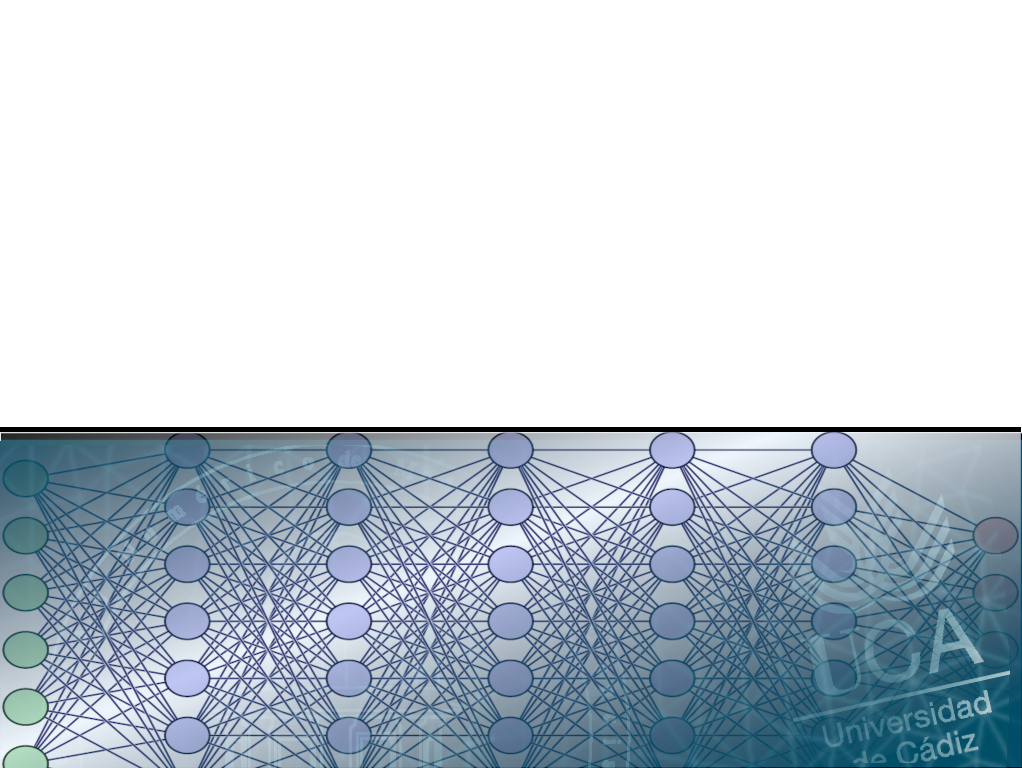
\includegraphics[width=\paperwidth,height=\paperheight]{frontpage_bg}}
\setbeamertemplate{footline}[default]
% <<<-------


% Write custom titlepage ------->>>
%\begin{frame}
%  \titlepage
%  \vspace{5cm}
%\end{frame}

% Set the background for the rest of the slides.
\setbeamertemplate{background}{}
 % {
\includegraphics[width=\paperwidth,height=\paperheight]{slide_bg}}


% Write all of the slides..........

% \begin{frame}{Outline}
%   \tableofcontents
% \end{frame}

% Start inserting infoline at the end
\setbeamertemplate{footline}[PHDtheme]
% <<<-------

%\newcommand{\imgdir}{Undefined, use renewcommand!}

%============================================================================
\section{Migración de neuroblastos en el cerebro adulto}
%============================================================================

%=====================================================================
\begin{frame}{¿Qué queremos modelar?}
%---------------------------------------------------------------------
\only<1>{
  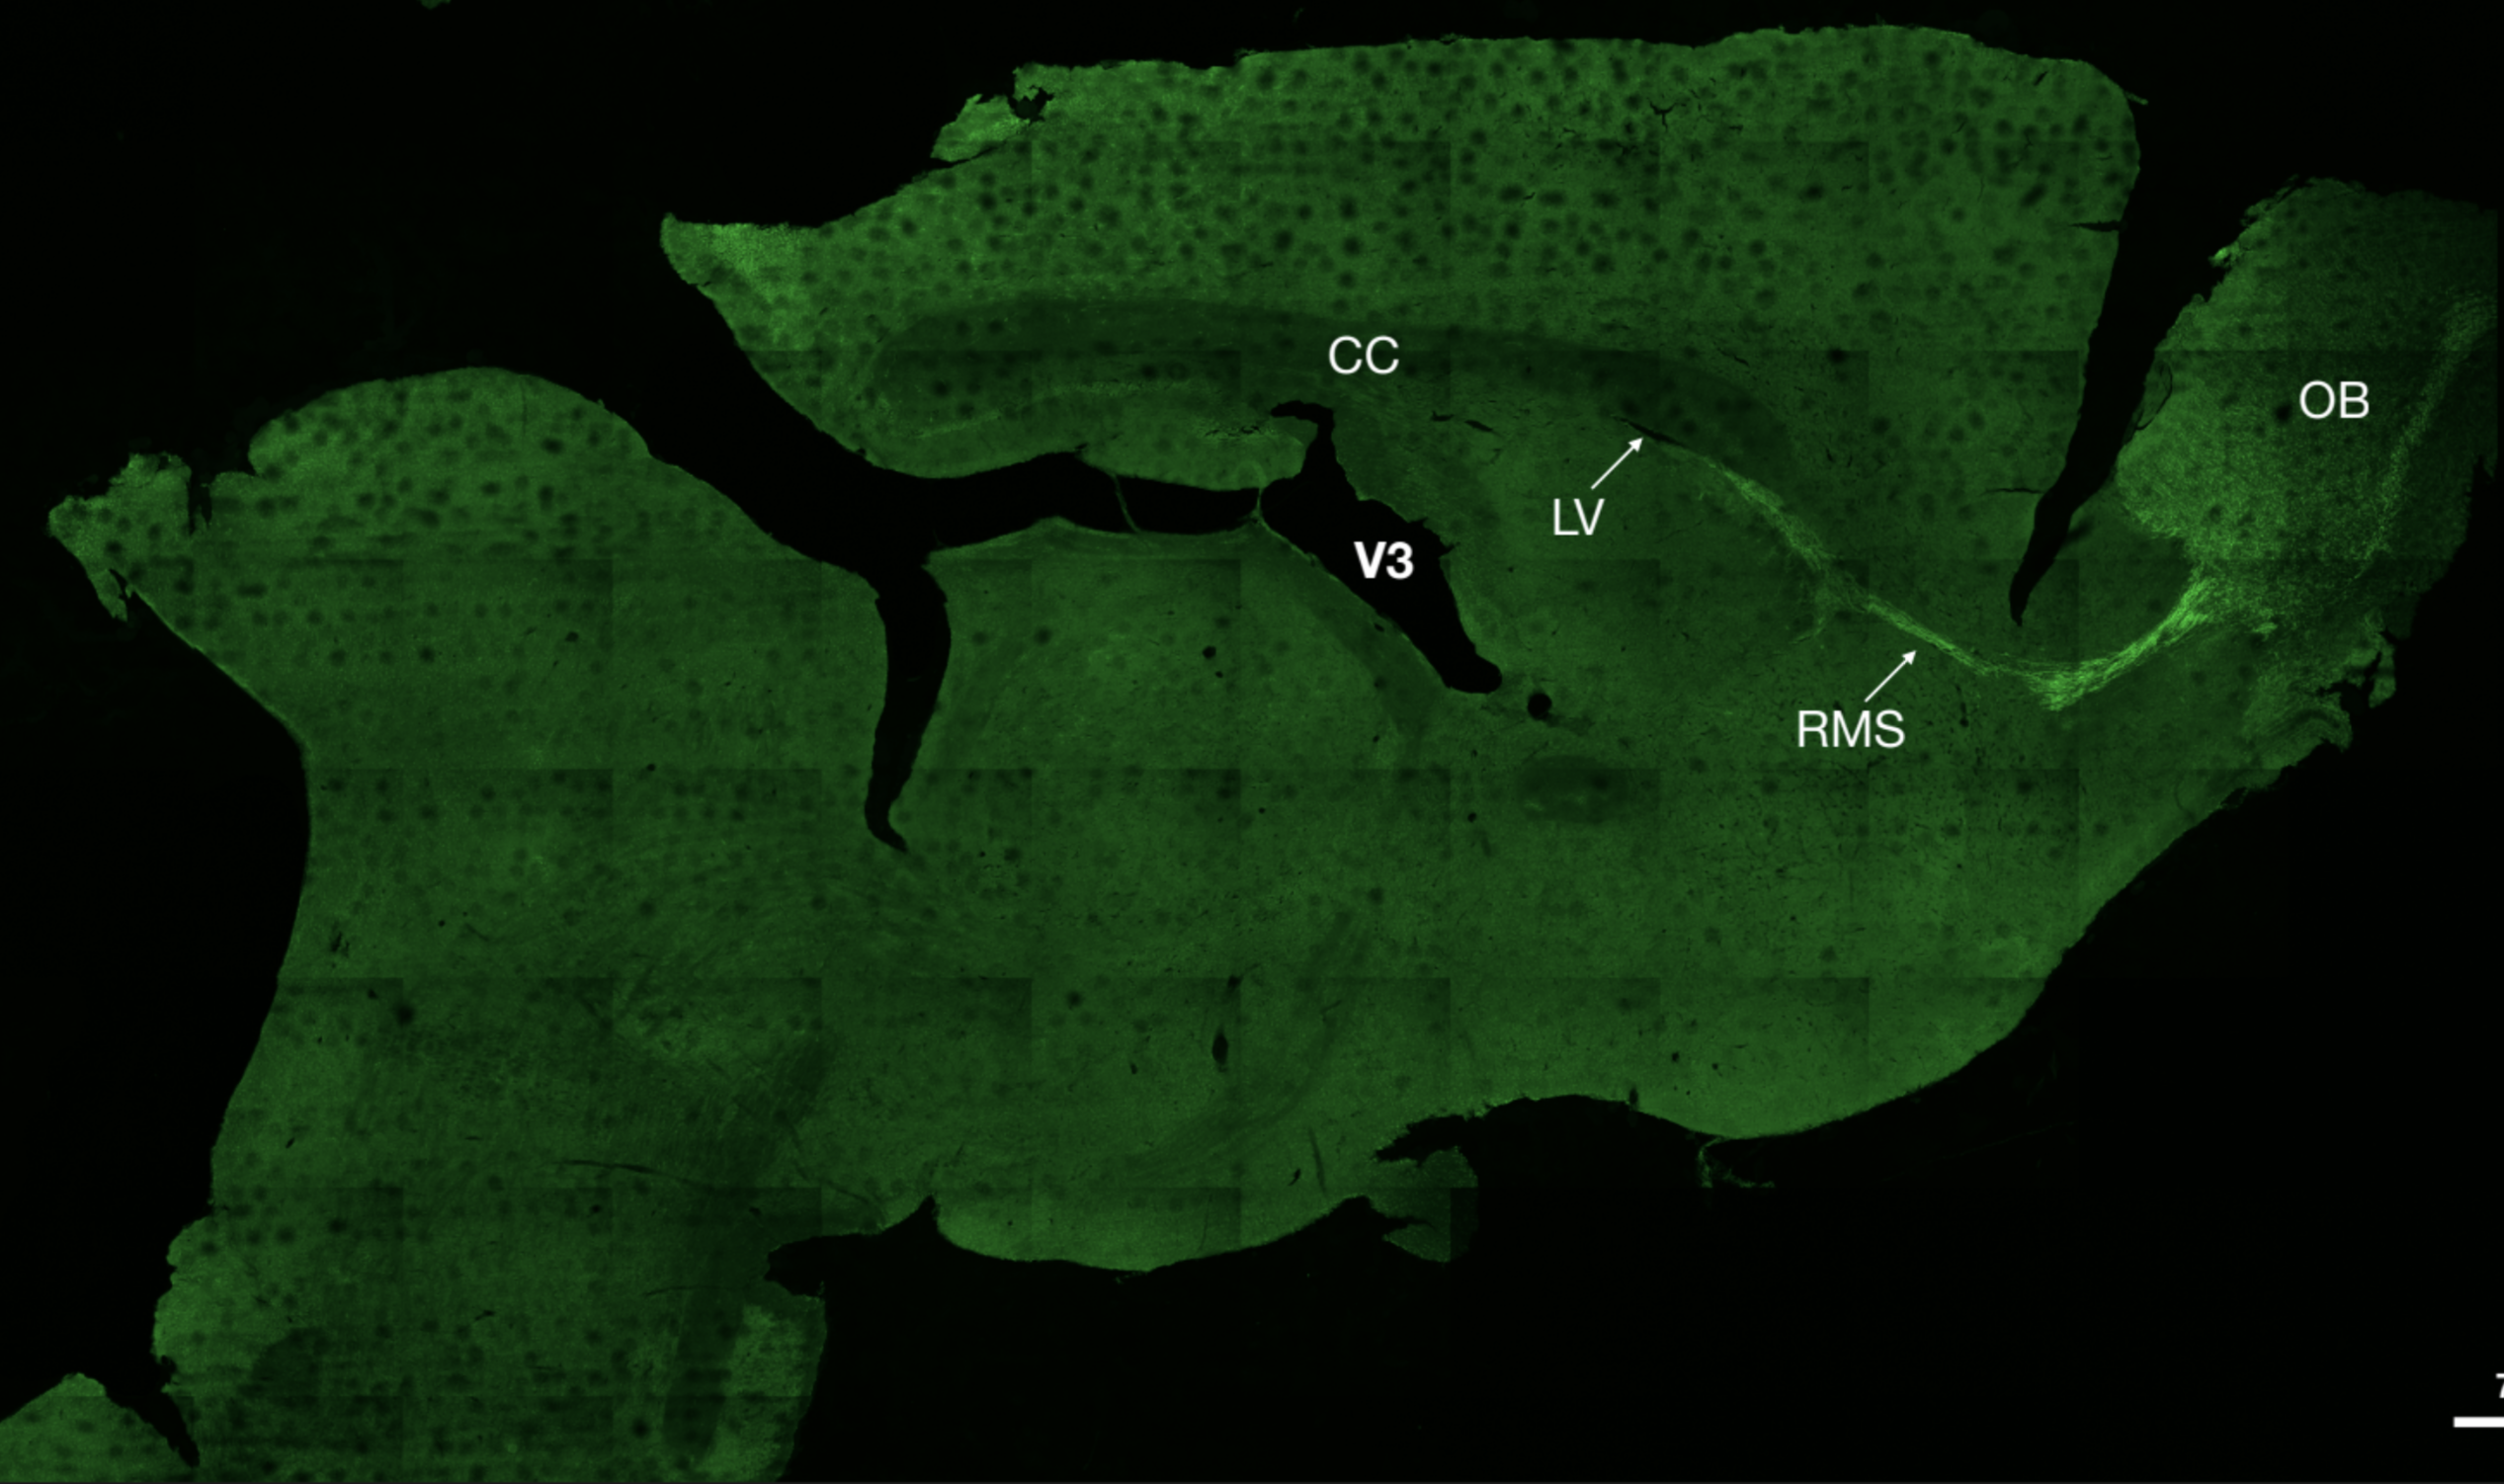
\includegraphics[width=0.95\linewidth]{cerebro-completo}}
  \only<2->{
  \includegraphics[width=0.95\linewidth]{via-rostral}}
\end{frame}

\begin{frame}{Primer objetivo: recuento de neuroblastos}
  \only<1>{
  	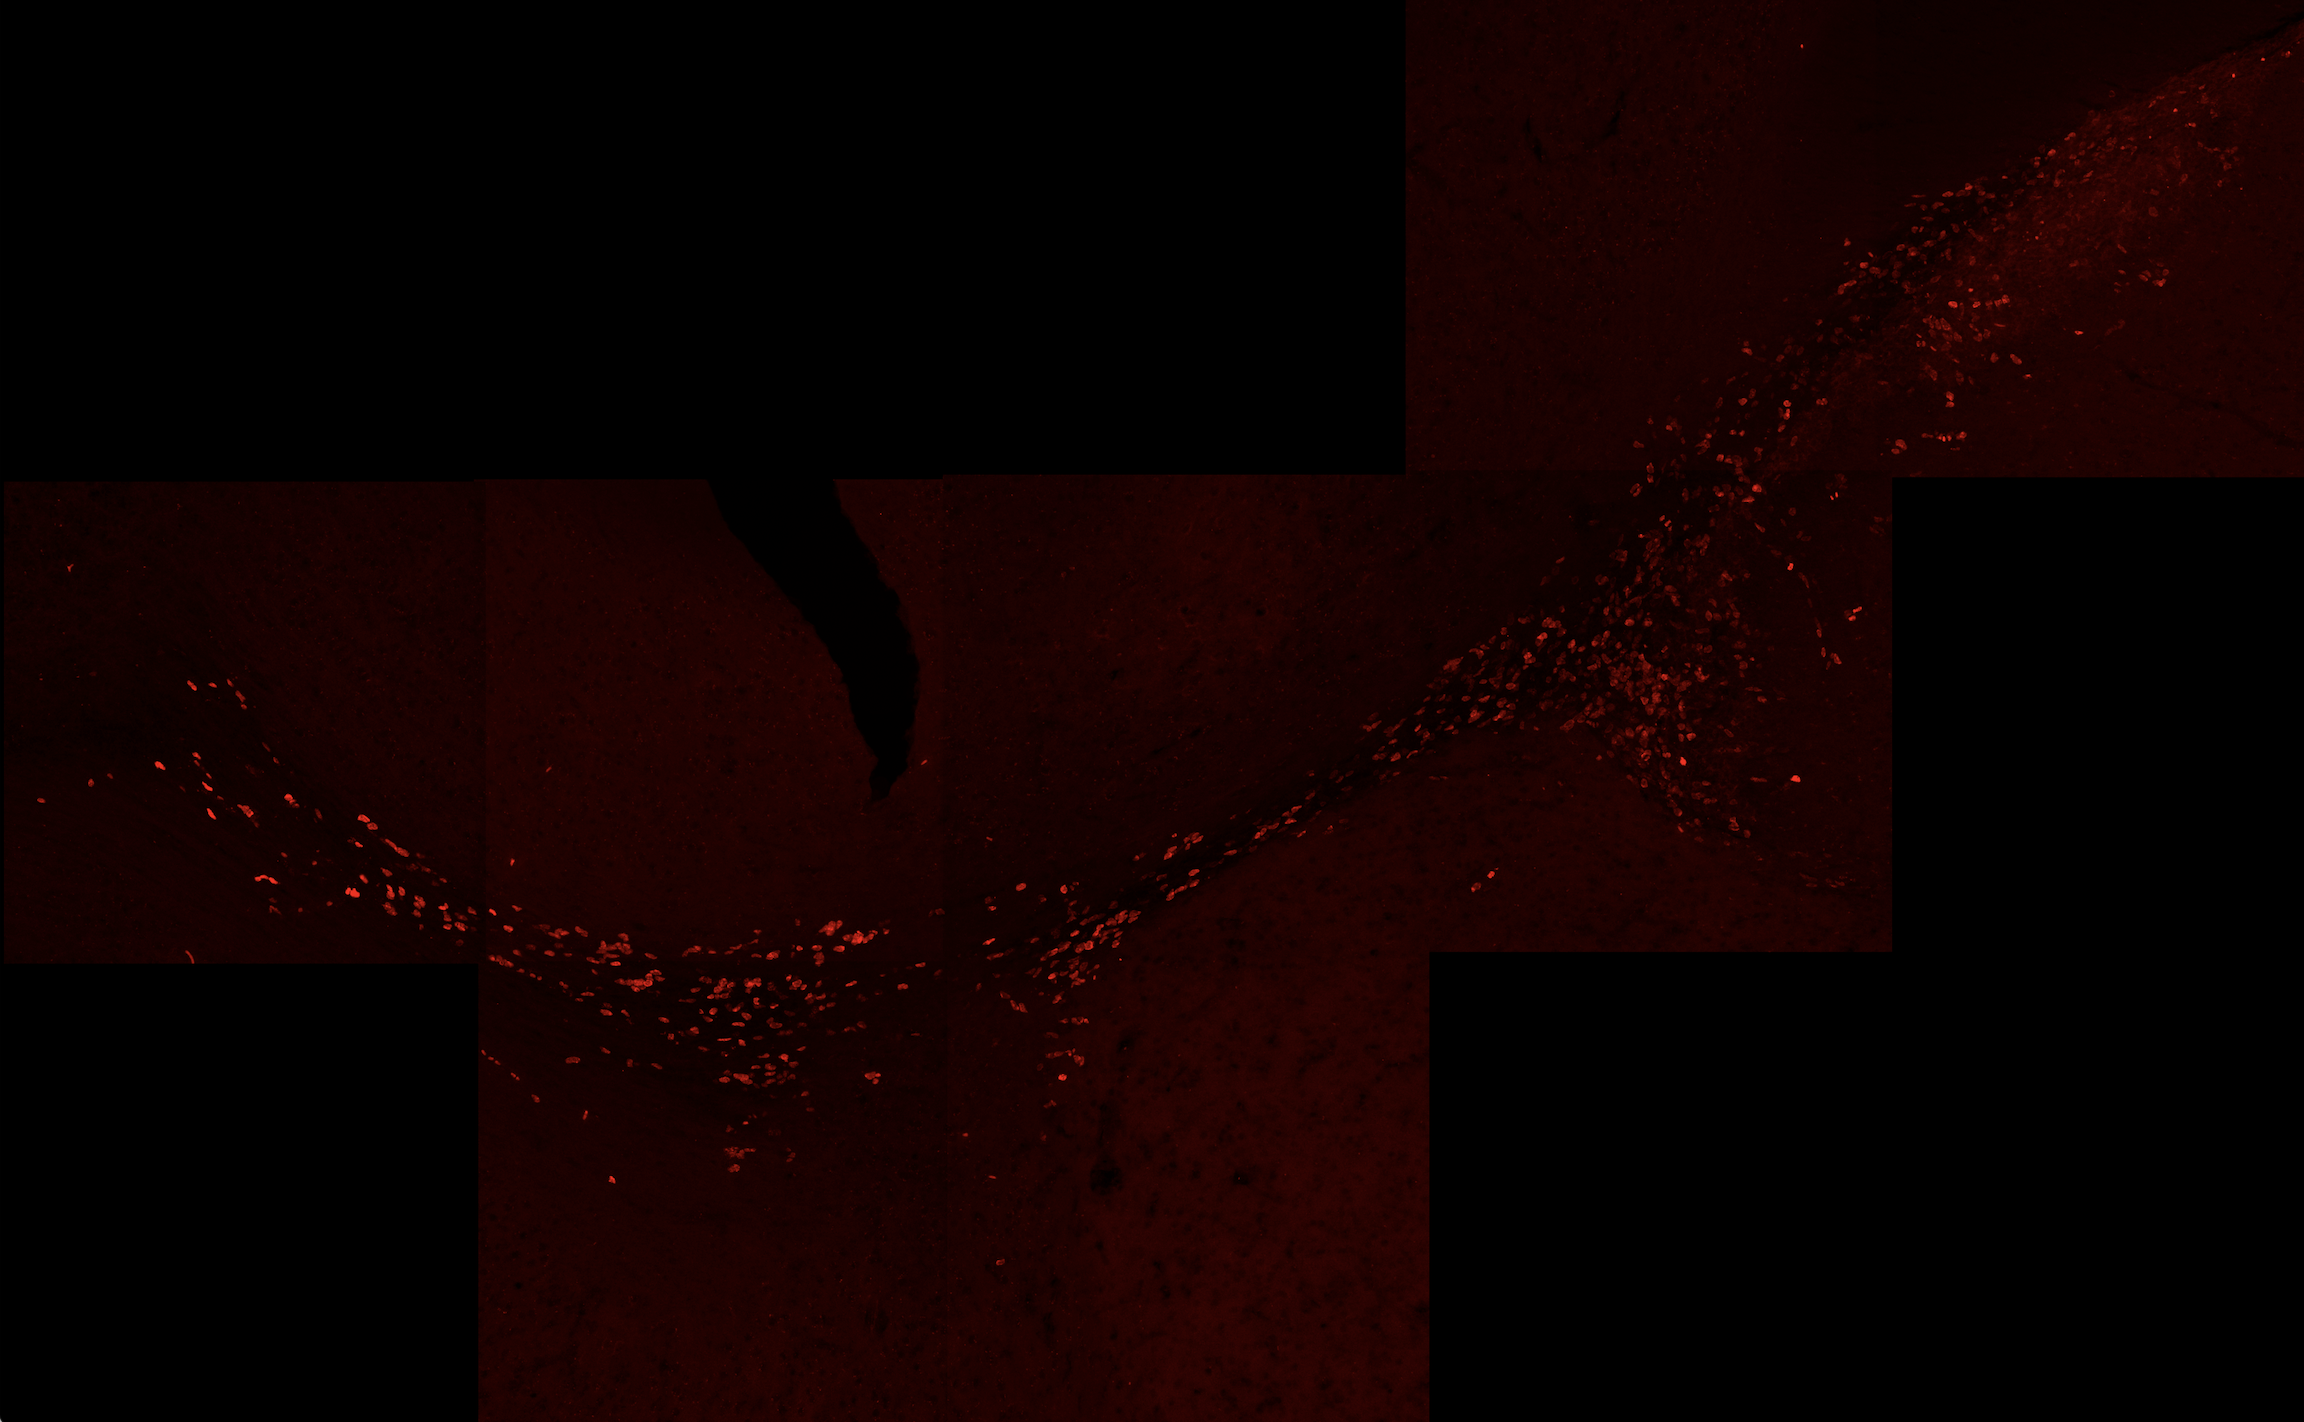
\includegraphics[width=0.95\linewidth]{via-roja}}
  \only<2->{
  	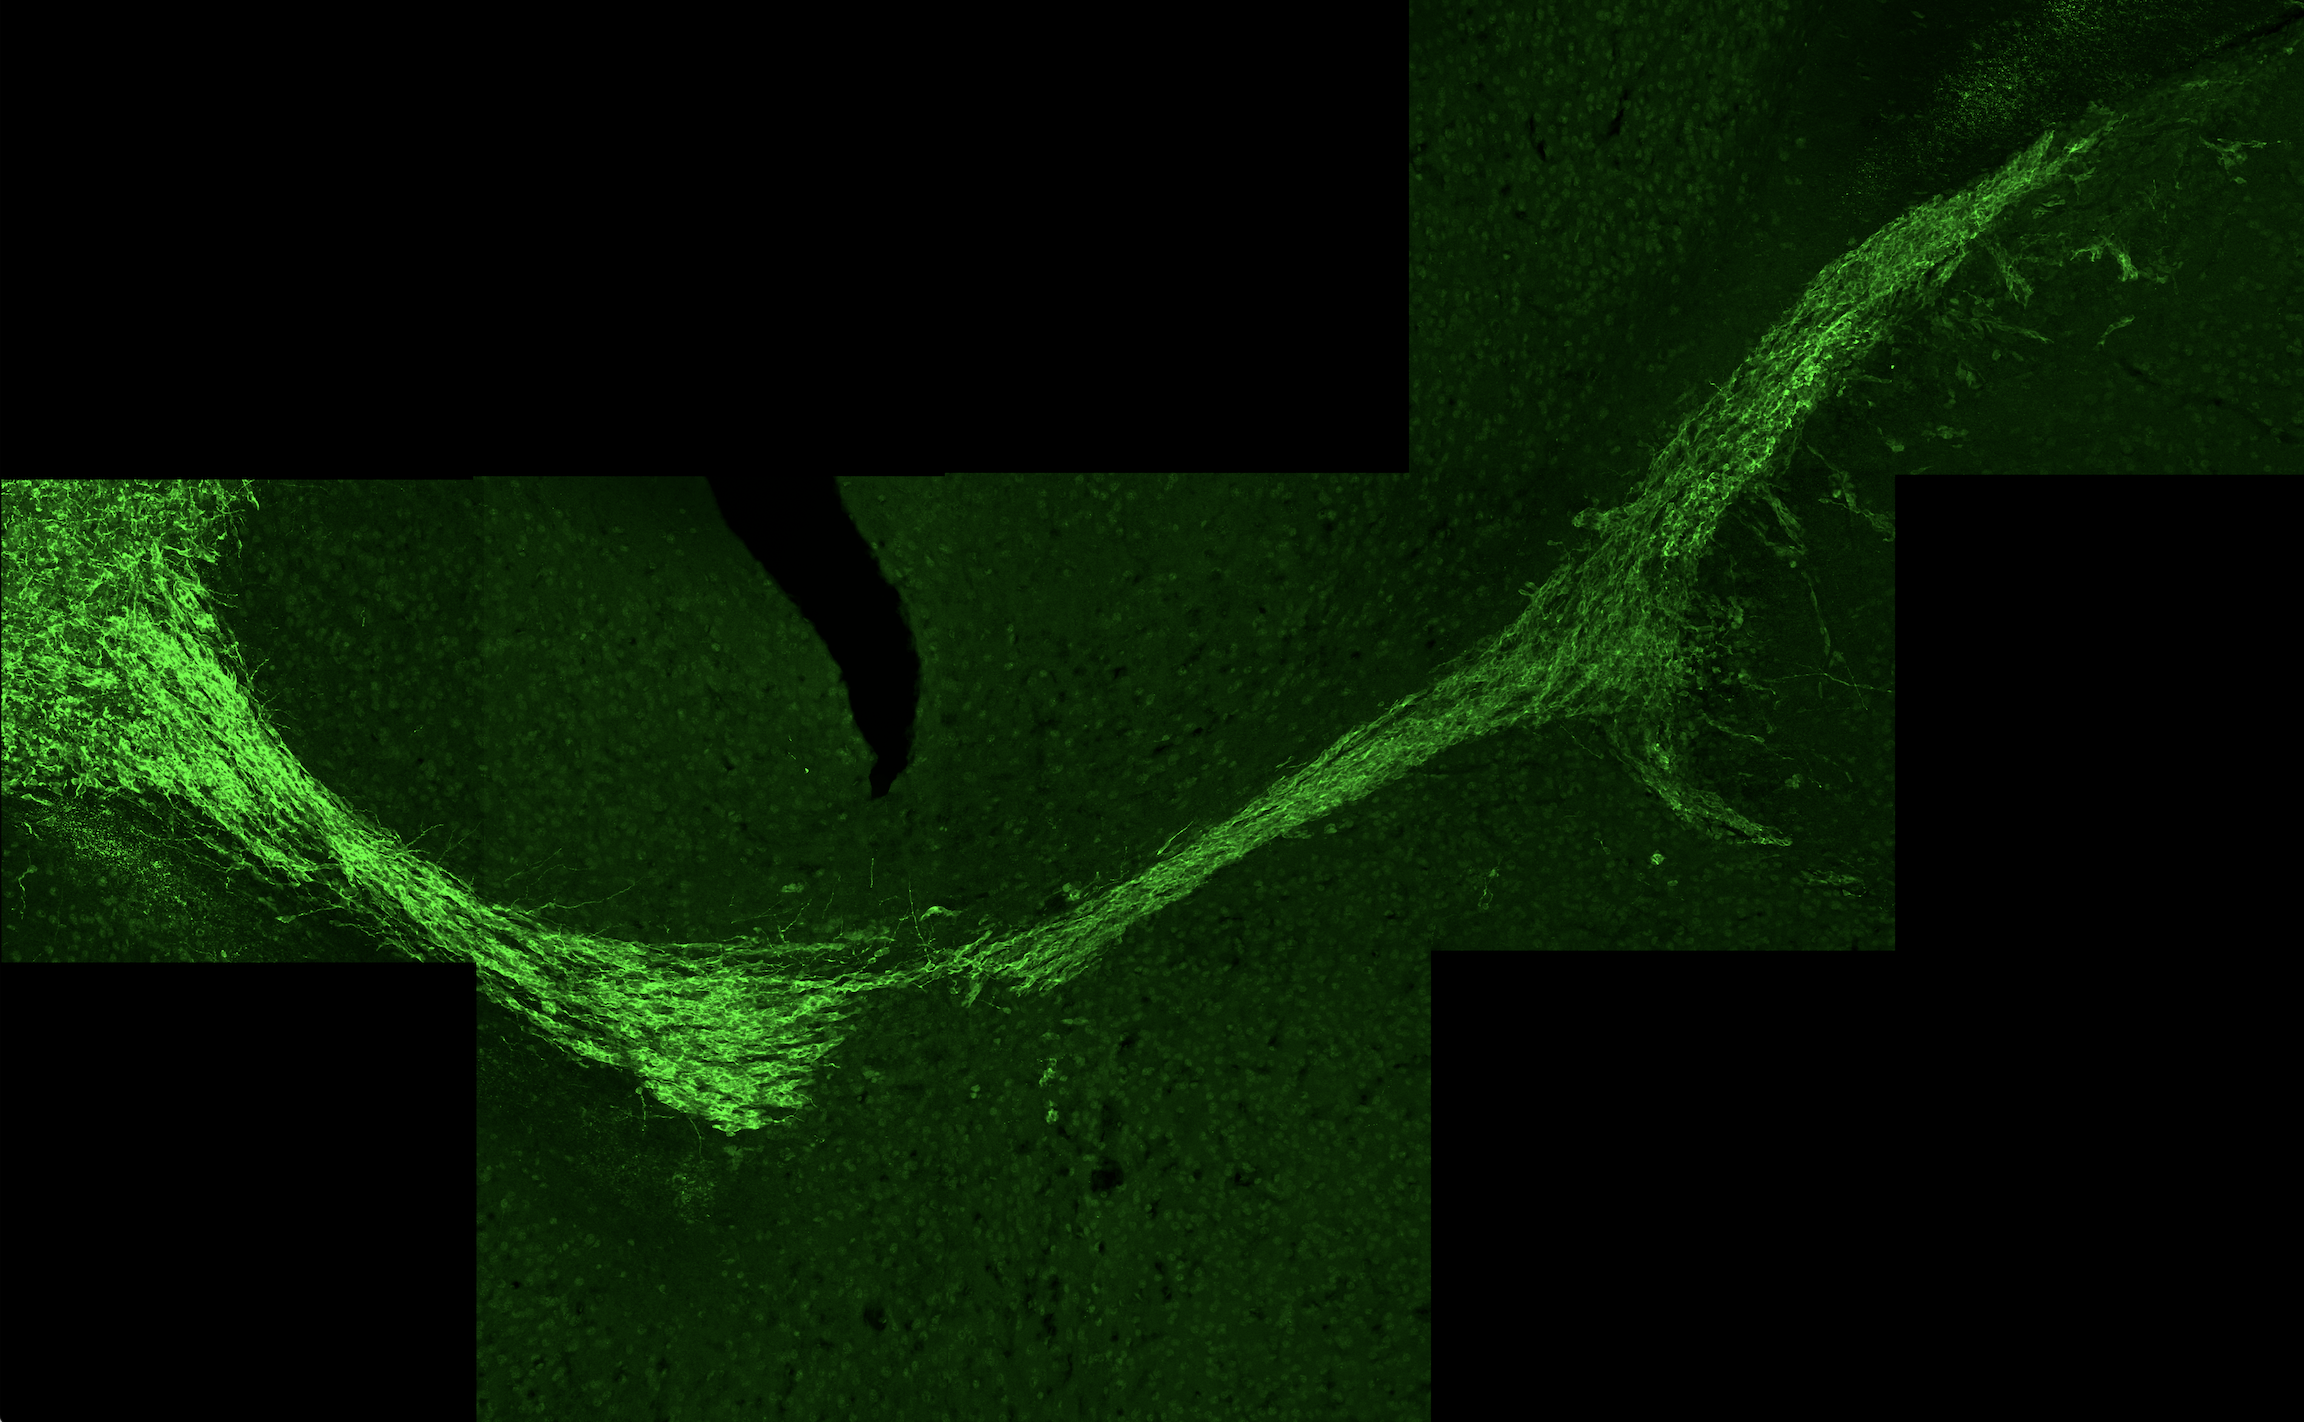
\includegraphics[width=0.95\linewidth]{via-verde}}
\end{frame}

\begin{frame}{Segundo objetivo: modelización y ajuste de parámetros}
	\begin{equation}
	\label{eq:neuroblast}
	\tau u_t + \X\, \nabla \cdot(u\nabla \O) + \alpha\, u - \gamma\, u \,1_{\NZdomain} 
	= \beta\, 1_{\SVZdomain}  
	\qquad\text{in}\enspace\Omega\times [0,T],
	\end{equation}
	\vspace{3mm}
	\begin{equation}
	\label{source}
	f_{\O}(x,y) = f_{\O}(\SO; x,y) 
	=  e^{((x-x_O)^2 + (y-y_O)^2)/\SO^2}.
	\end{equation}
	\vspace{3mm}
	\begin{equation} 
	\label{ob}
	\left\{ \begin{aligned} \Olf-\nabla\cdot (\mu_\CCdomain\,\nabla \Olf) &= f_{\O}  \quad  \text{ in } \Omega, \\
	\Olf &= f_{\O}  \quad \text{ on } \partial\Omega.
	\end{aligned}
	\right.
	\end{equation}
\end{frame}

\begin{frame}{Cerebro virtual}
	Malla
	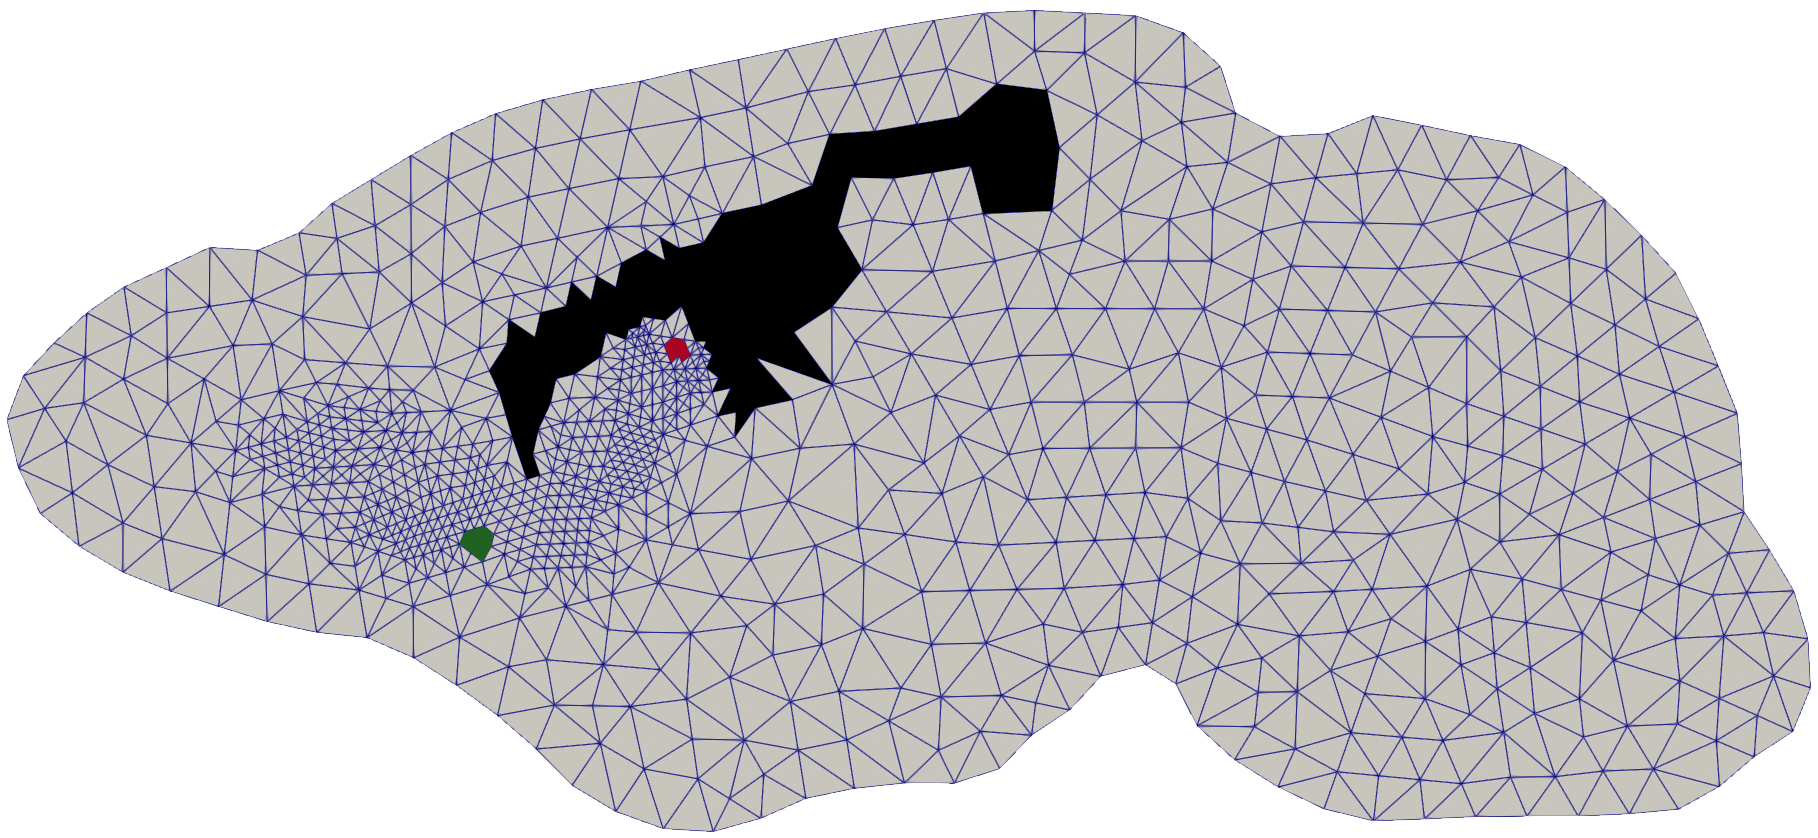
\includegraphics[width=0.95\linewidth]{brain-mesh.png}
\end{frame}

\begin{frame}{Modelización de la atracción}
Gradiente del bulbo olfatorio: parámetro $\sigma$
 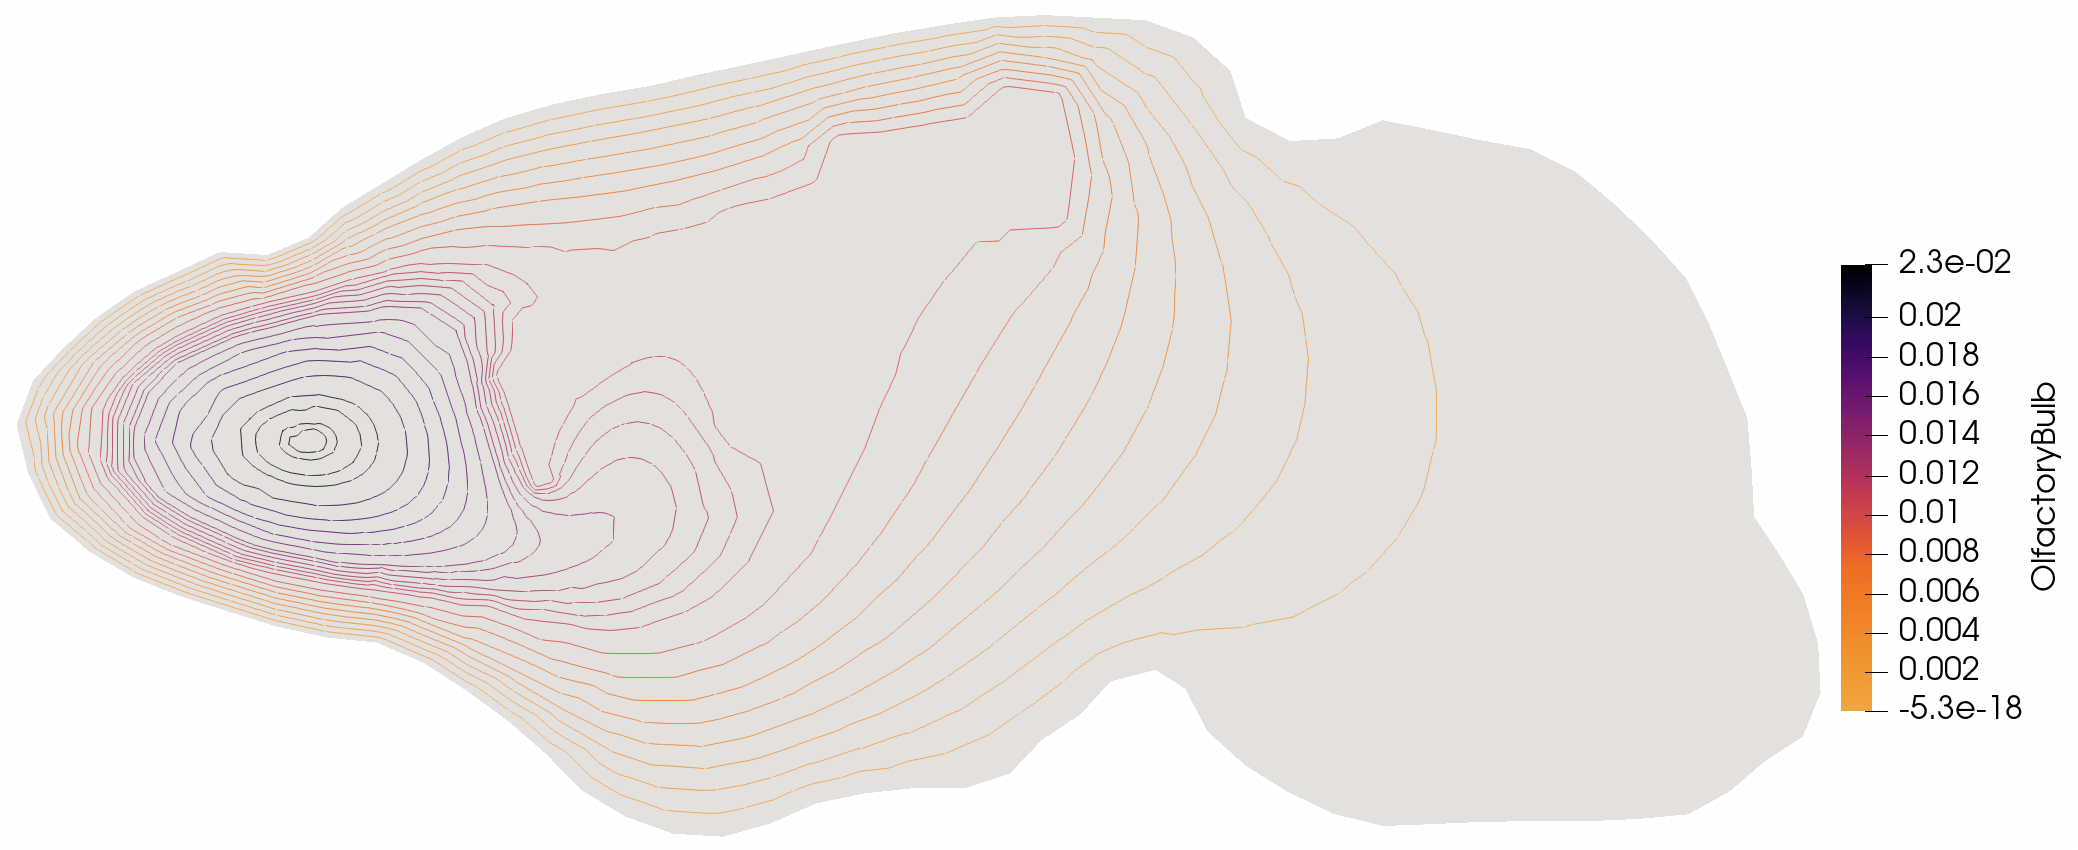
\includegraphics[width=0.95\linewidth]{ob.png}
\end{frame}
\begin{frame}{Modelización del movimiento}
	Vía rostral: parámetros $\alpha, \beta, \X, \gamma$
	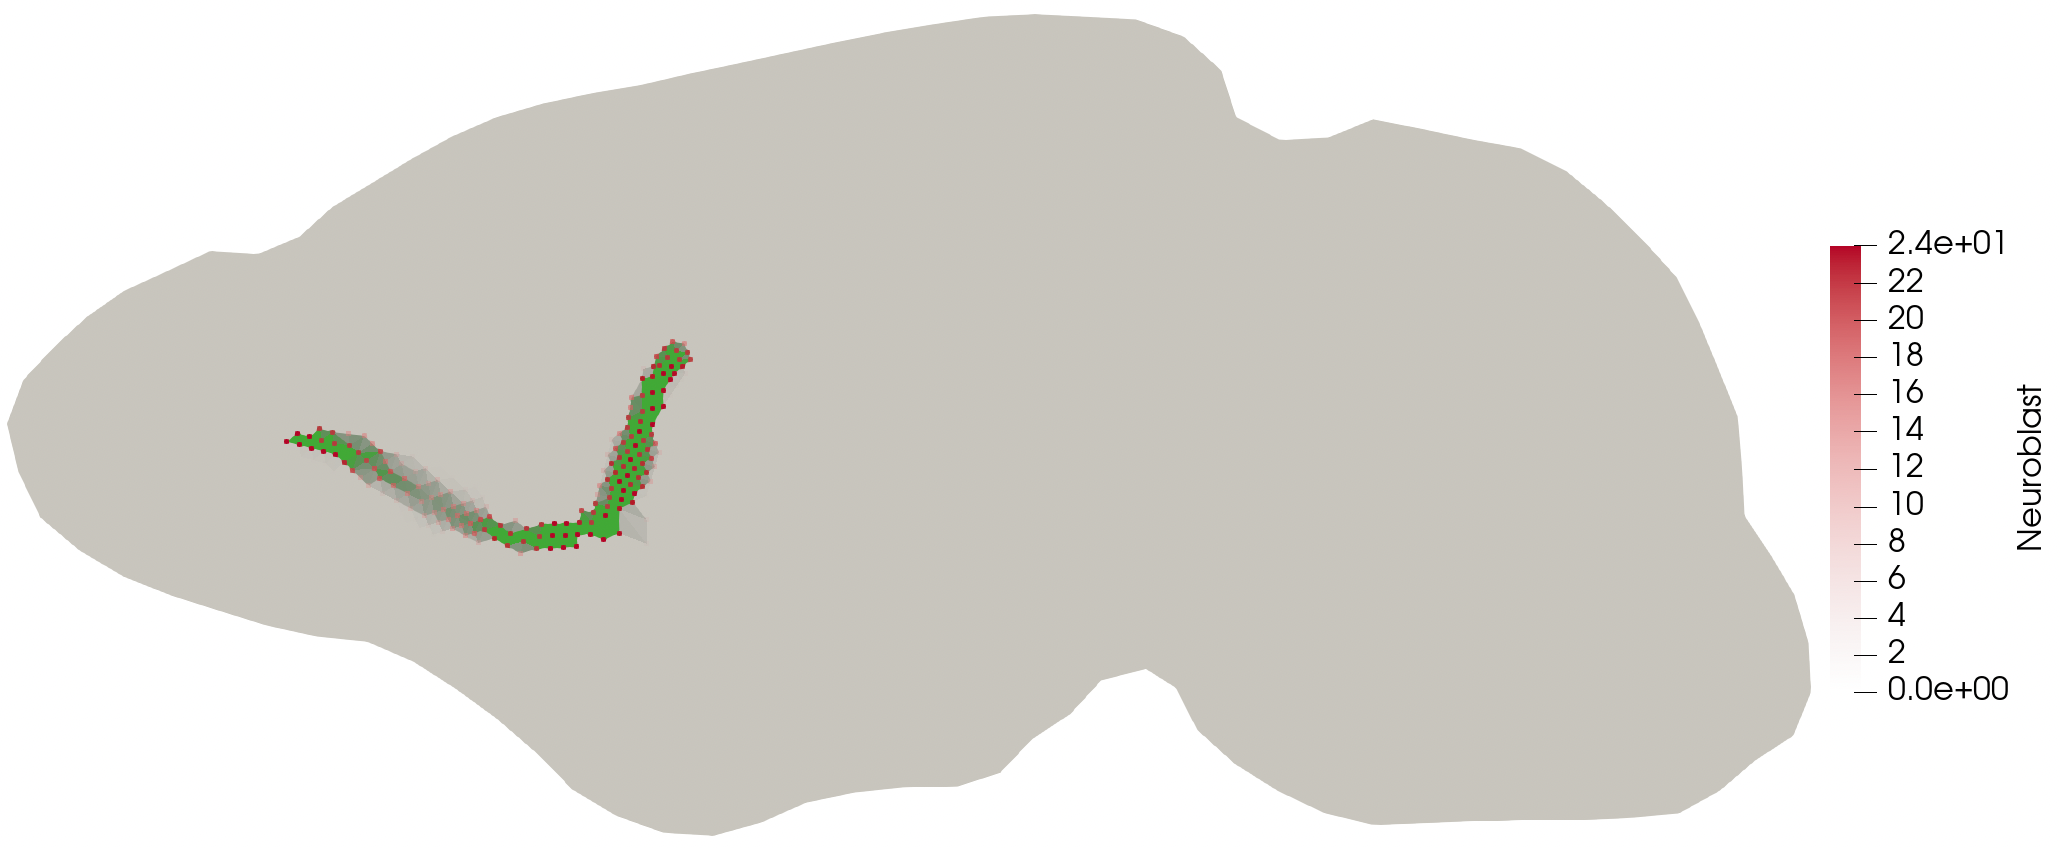
\includegraphics[width=0.95\linewidth]{steady-opt.png}
\end{frame}




%\include{dan1}
%
%% Beamer style >>>>>>>>>>>>>>>>>>>>>>>>>

\setbeamertemplate{enumerate item}[mycircle]

\setbeamertemplate{frametitle continuation}[from second][] % No automatic symbols I II II
%<<<<<<<<<<<<< beamer style

%\title{Redes Neuronales y otros Artefactos Matemáticos\vspace{-0.5em}}
%\author[J.R. Rodr\'{\i}guez Galv\'an]{\em\structure{Daniel Acosta Soba, Noelia Ortega Román, Álex Pérez Fernández, Rafa Rodríguez Galván}\vspace{-1.5em}}
%\date{\scriptsize{Facultad de Ciencias, Universidad de C\'adiz}\\[0.9em]\small Día Internacional de las Matemáticas («día {\Huge$\pi$}»), 2023}

% XeLaTeX font choosing
% \usepackage{fontspec}%{xltxtra} %fontspec}
% \setsansfont{Fontin Sans}
% \setsansfont{Lato}


\setcounter{tocdepth}{1}
\newcommand{\Olf}{\mathcal{O}}
\newcommand{\SVZdomain}{\text{\it SVZ}}
\newcommand{\NZdomain}{\text{\it NZ}}
\newcommand{\CCdomain}{{\text{\it CC}}}
\newcommand{\CCexp}{\mu_{CC}}
\newcommand{\tCCexp}{\tilde{\mu}_{CC}}
\def\SO{\sigma}
\def\X{\chi}
\def\D{\mathscr{D}}
\def\T{\mathcal{T}}
\def\E{\mathcal{E}}
\def\S{\mathcal{S}}
\def\N{\mathbb{N}}
\def\P{\mathbb{P}}
\def\O{\mathcal{O}}

%
% Bibliography
%
%\usepackage{natbib}

% To list each bibliographic entry in a line
\setbeamertemplate{bibliography entry title}{}
\setbeamertemplate{bibliography entry location}{}
\setbeamertemplate{bibliography entry note}{}

% ... end of preamble.

\AtBeginSection{\frame{\sectionpage}}

\colorlet{inputcolor}{green!60!black}
\colorlet{hiddencolor}{blue!60!black}
\colorlet{outcolor}{red!60!black}

%======================================================================

%======================================================================

% Tikz style and beamer template ------->>>
\tikzstyle{every picture}+=[remember picture]
\tikzstyle{na} = [baseline=-.5ex]
\tikzstyle{phd} = [baseline=-.6ex,
  box/.style={rectangle, draw=PHDblueC, thick, fill=PHDblueA,
    align=center, rounded corners, minimum height=1.6em},
  boxB/.style={rectangle, draw=PHDredA, thick, fill=PHDblueA,
    align=center, rounded corners, minimum height=1.6em}]
\tikzstyle{phdB} = [baseline=-.7ex,
  box/.style={rectangle, draw=PHDblueC, thick, fill=PHDblueA,
    align=center, rounded corners, minimum height=1.6em},
  boxB/.style={rectangle, draw=PHDredA, thick, fill=PHDblueA,
    align=center, rounded corners, minimum height=1.6em}]
\tikzstyle{myarrow} = [->,>=latex, PHDredA, shorten >=4pt,
  opacity=.6, line width=0.6mm]
\tikzstyle{myarrow2} = [->,>=latex, PHDblueC, shorten >=4pt, opacity=.2, line width=0.4mm]
\tikzstyle{myarrow3} = [
     opacity=.7,
%    >=triangle 60,              % Nice arrows; your taste may be different
    node distance=6mm and 60mm, % Global setup of box spacing
    every join/.style={norm},   % Default linetype for connecting
                                % boxes
    line width=0.6mm,
    PHDredA,
    ->
    ]
\setbeamertemplate{background}
 {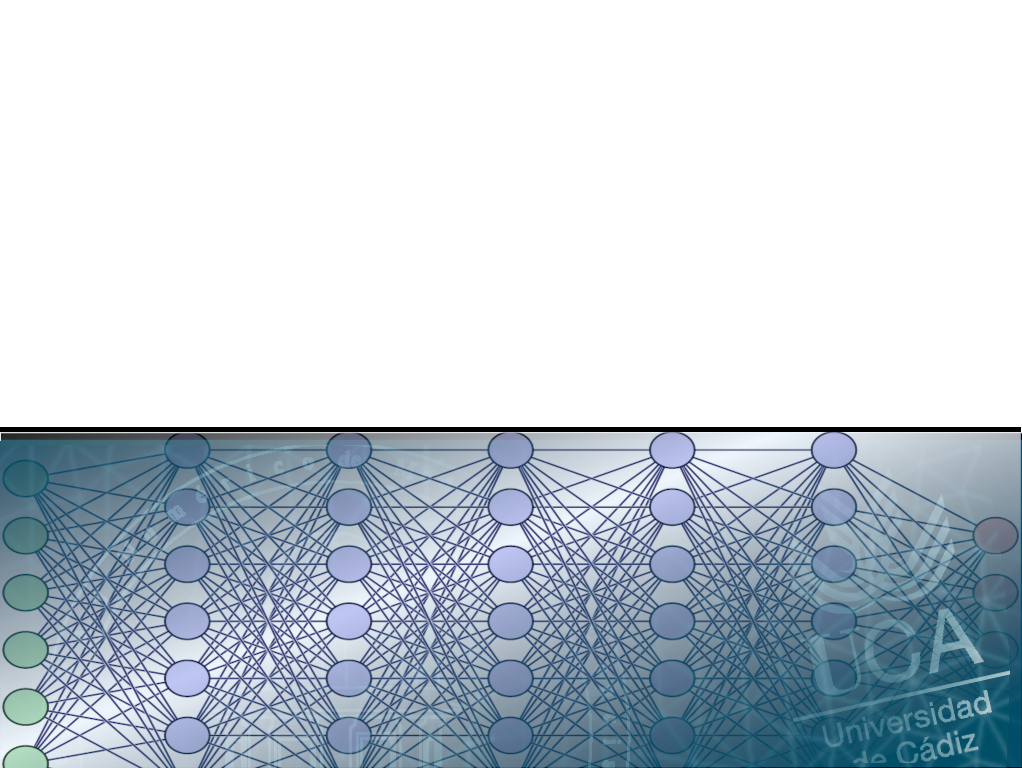
\includegraphics[width=\paperwidth,height=\paperheight]{frontpage_bg}}
\setbeamertemplate{footline}[default]
% <<<-------


% Write custom titlepage ------->>>
%\begin{frame}
%  \titlepage
%  \vspace{5cm}
%\end{frame}

% Set the background for the rest of the slides.
\setbeamertemplate{background}{}
 % {
\includegraphics[width=\paperwidth,height=\paperheight]{slide_bg}}


% Write all of the slides..........

% \begin{frame}{Outline}
%   \tableofcontents
% \end{frame}

% Start inserting infoline at the end
\setbeamertemplate{footline}[PHDtheme]
% <<<-------

%\newcommand{\imgdir}{Undefined, use renewcommand!}

%============================================================================
\section{Migración de neuroblastos en el cerebro adulto}
%============================================================================

%=====================================================================
\begin{frame}{¿Qué queremos modelar?}
%---------------------------------------------------------------------
\only<1>{
  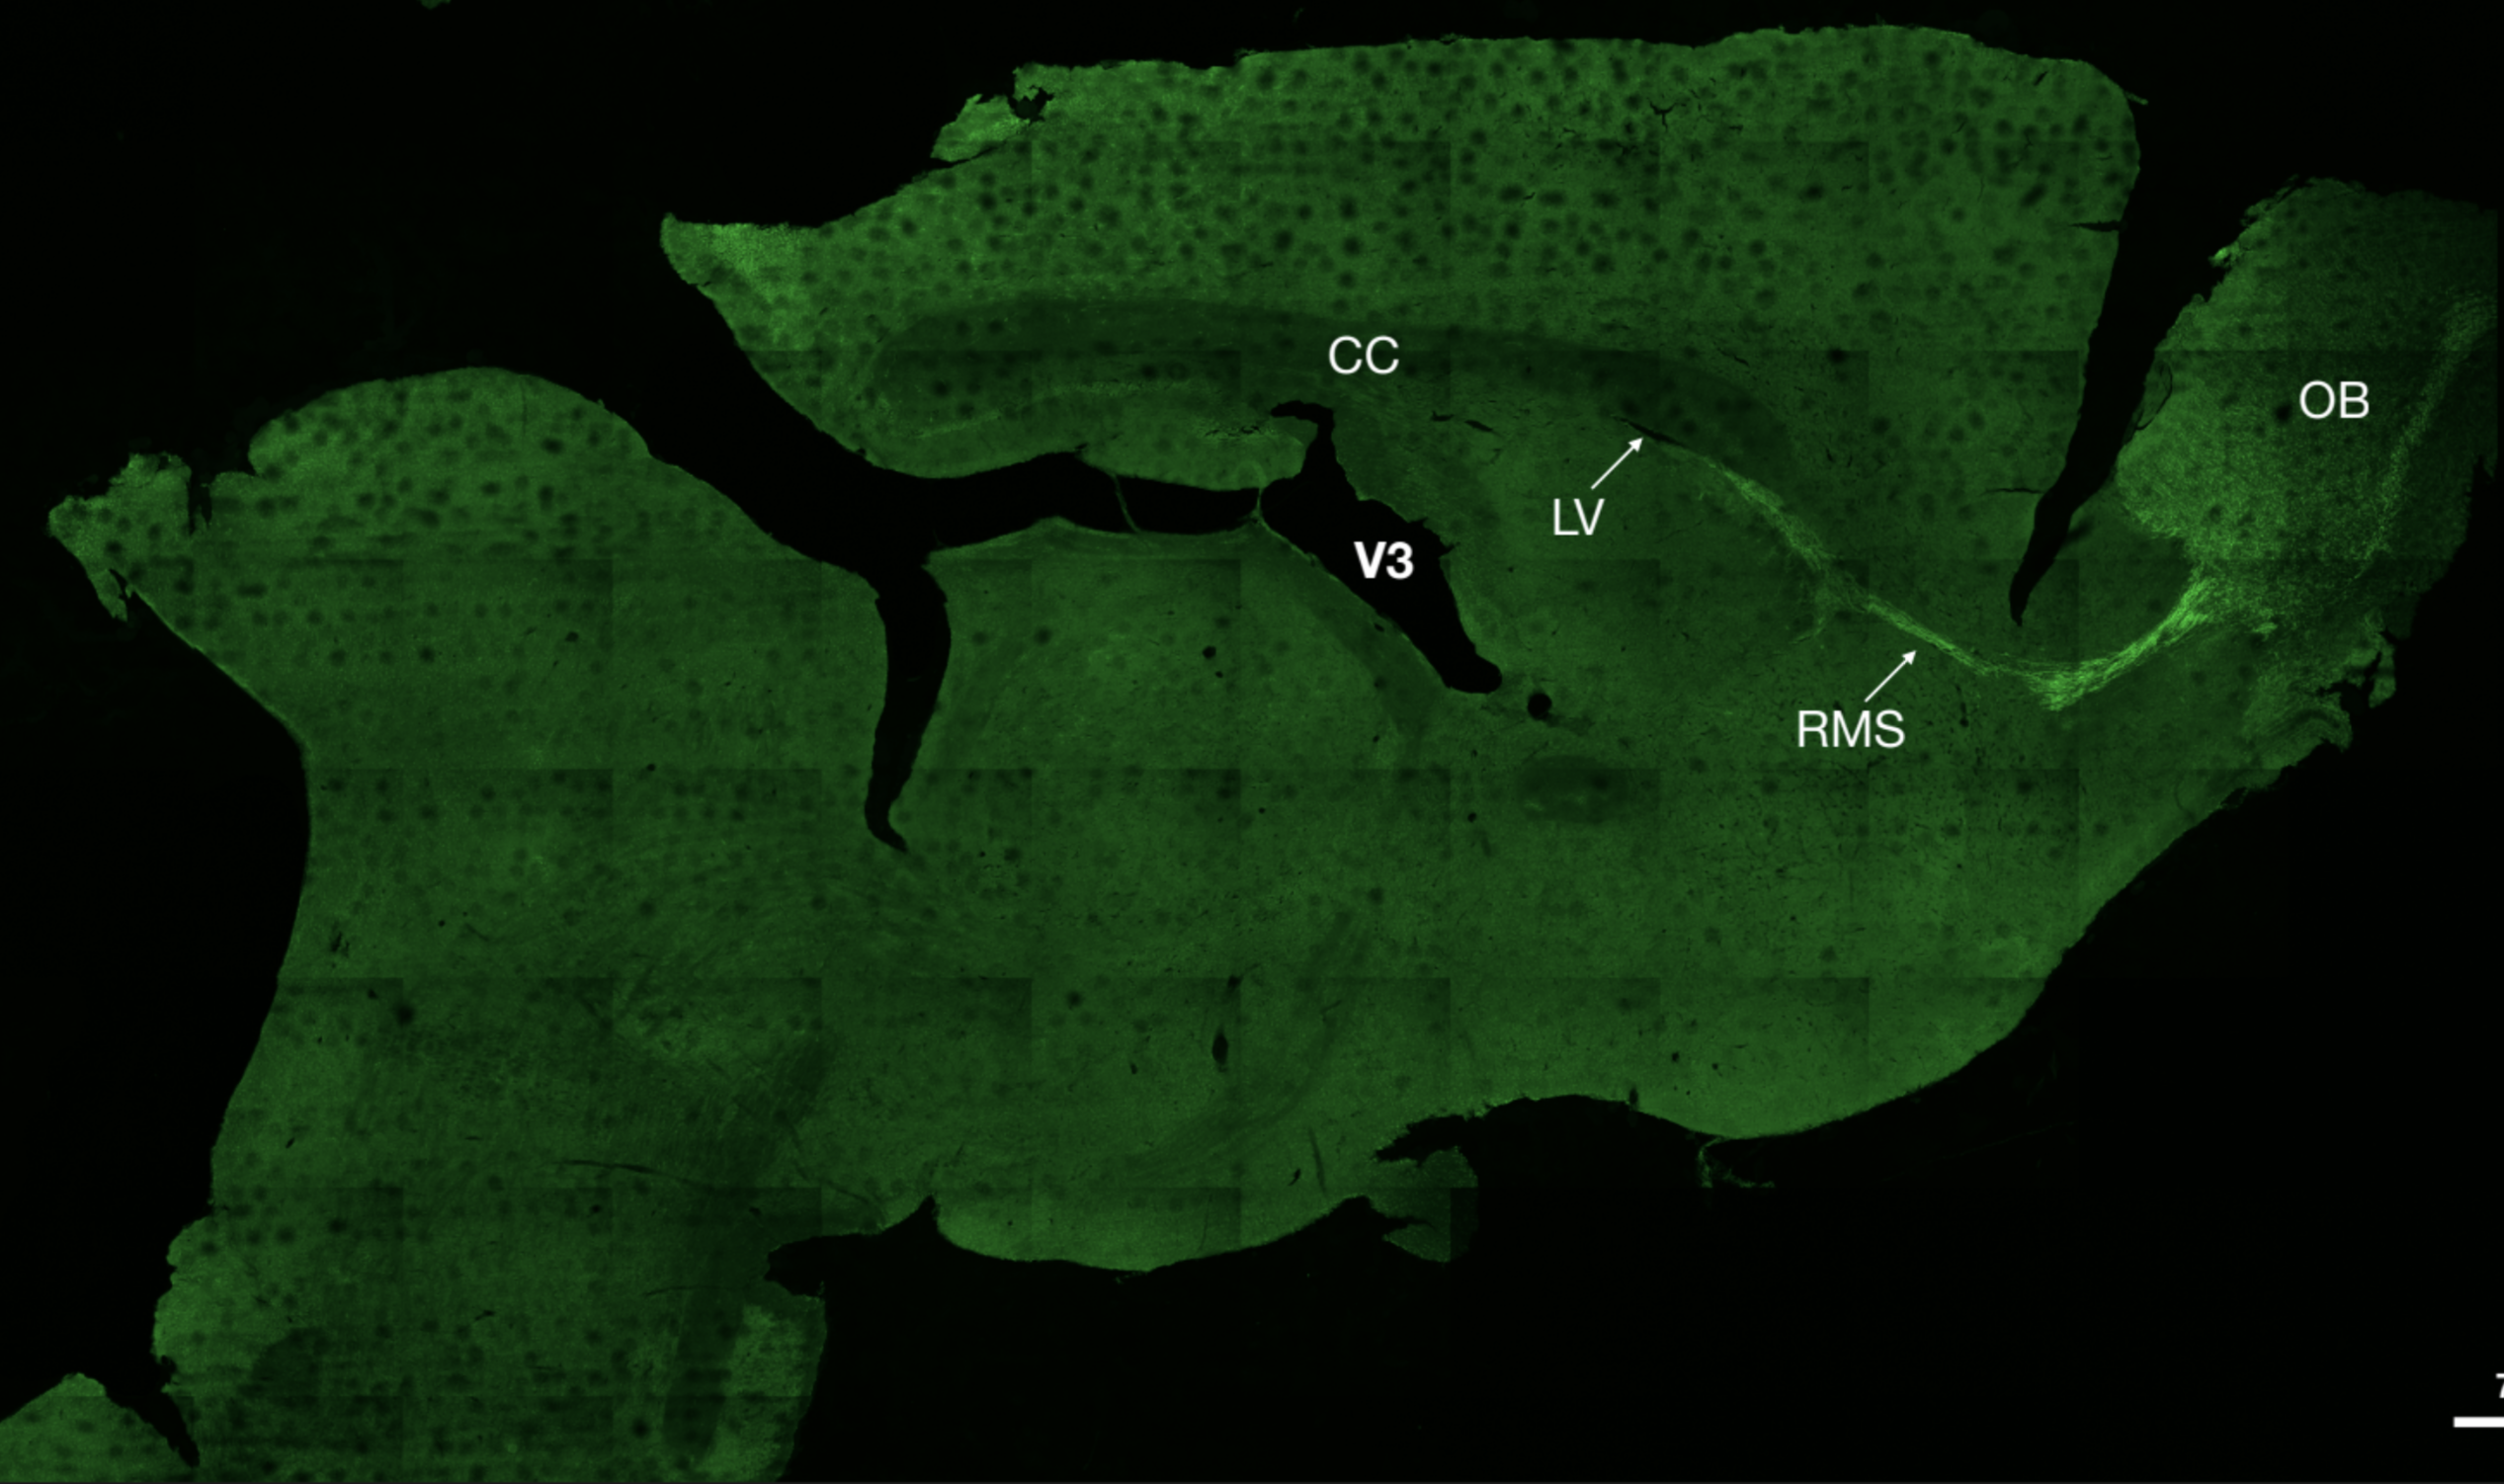
\includegraphics[width=0.95\linewidth]{cerebro-completo}}
  \only<2->{
  \includegraphics[width=0.95\linewidth]{via-rostral}}
\end{frame}

\begin{frame}{Primer objetivo: recuento de neuroblastos}
  \only<1>{
  	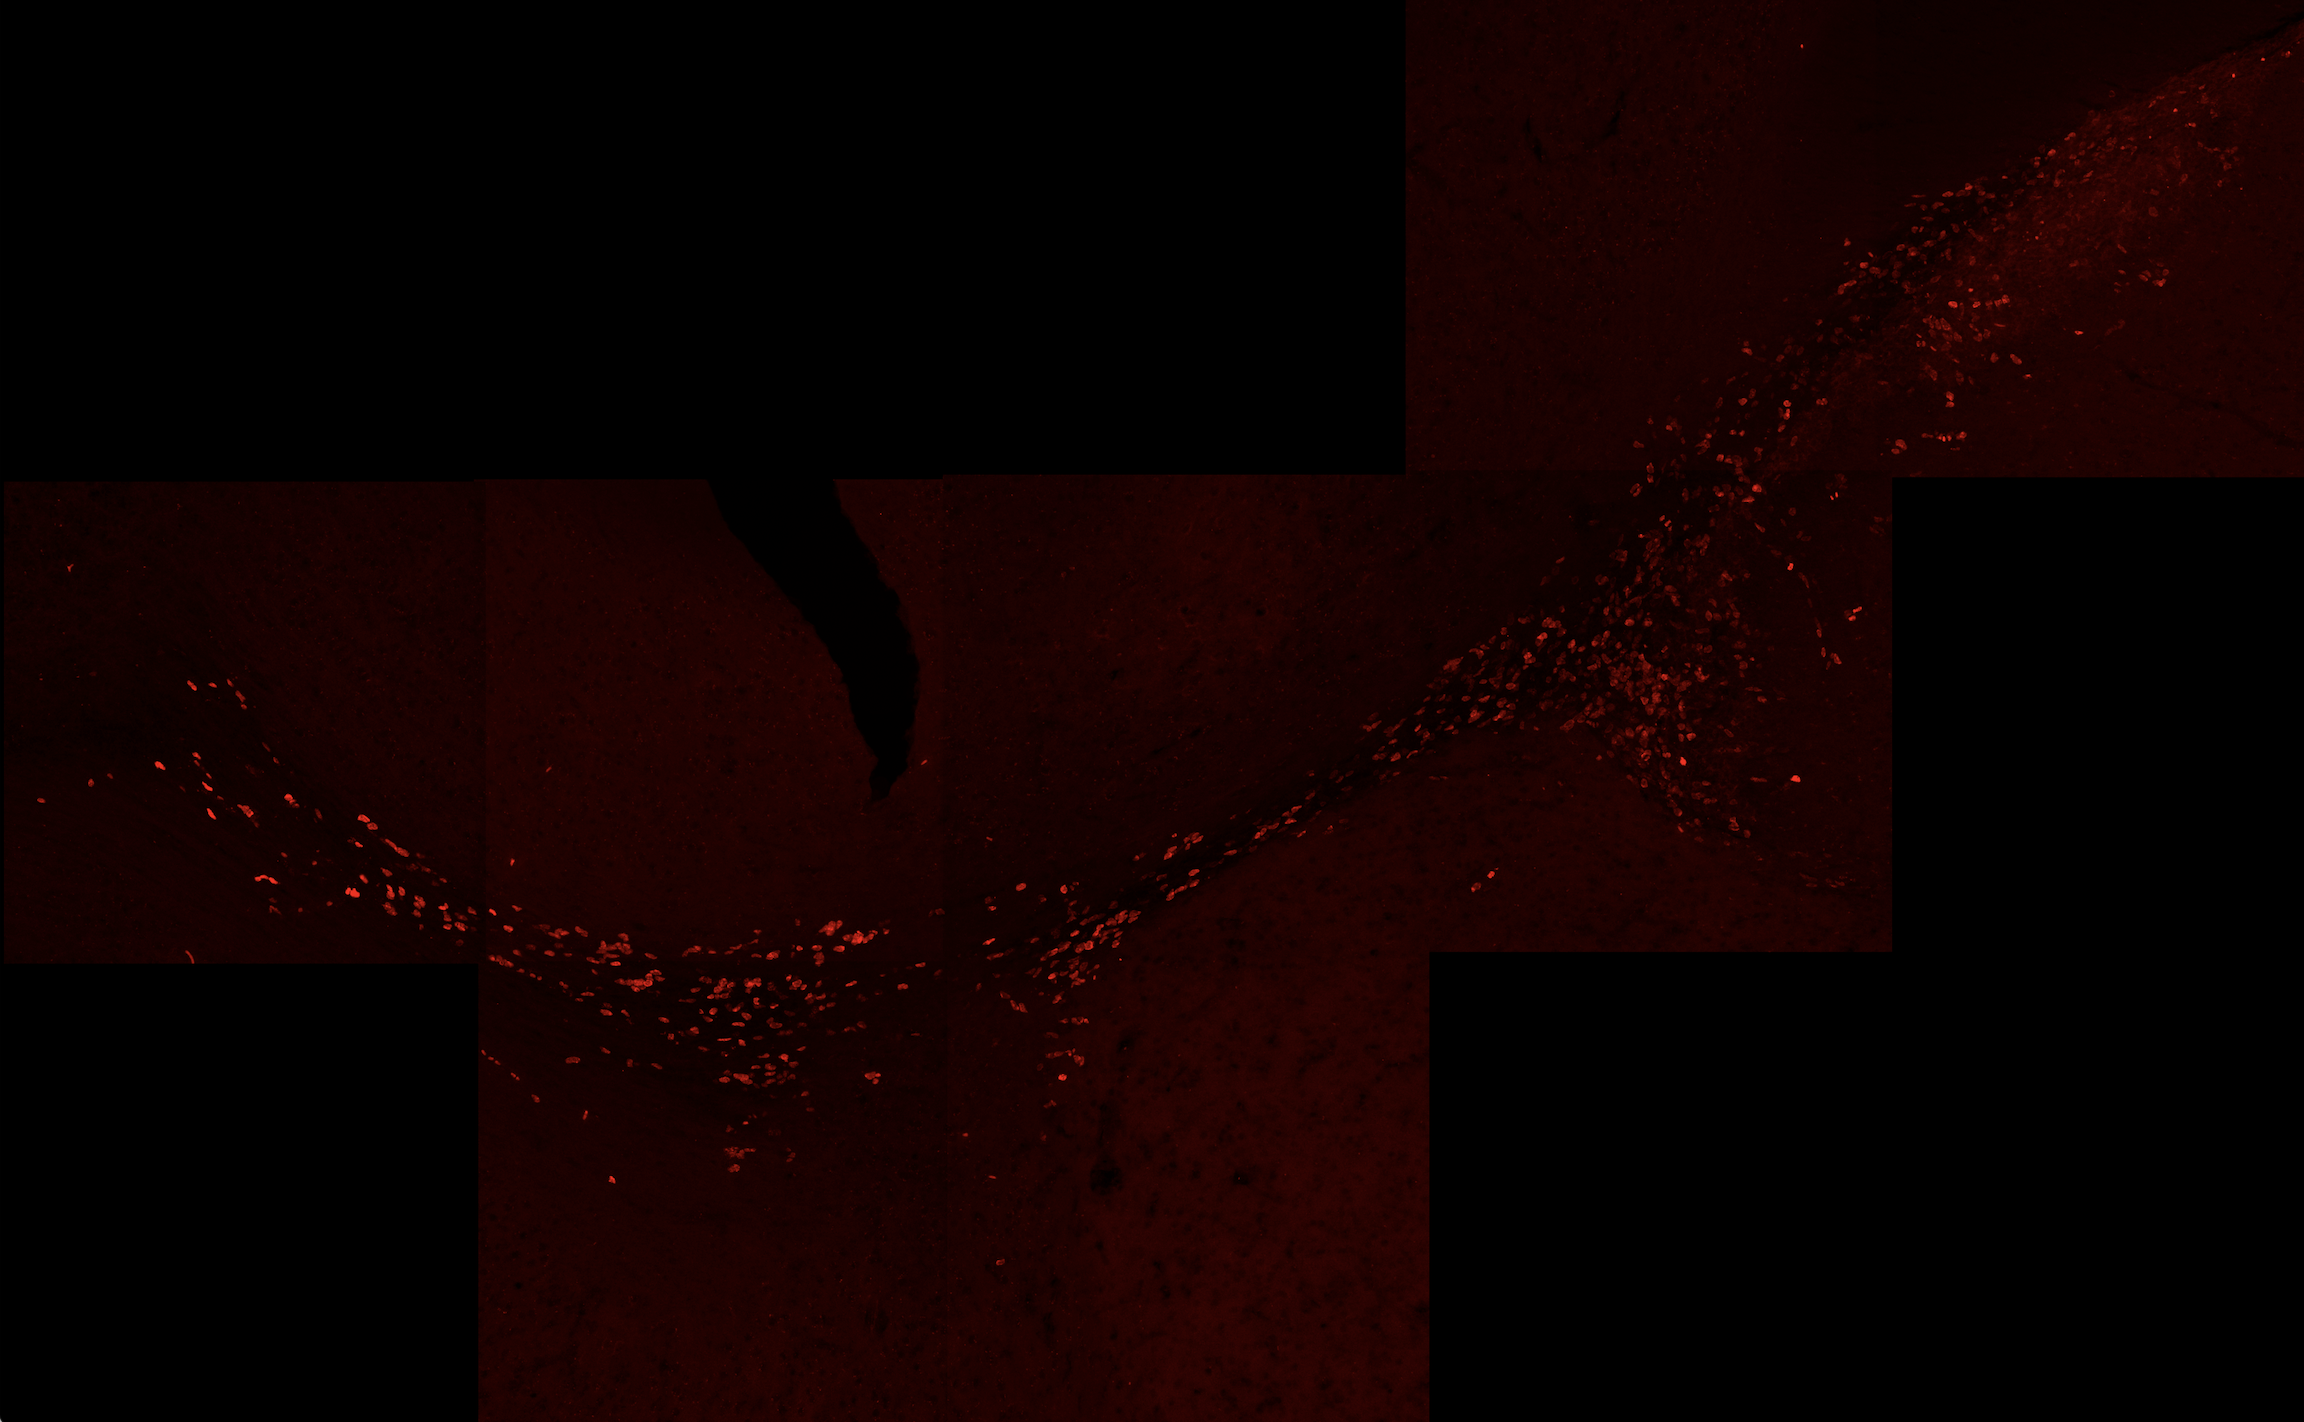
\includegraphics[width=0.95\linewidth]{via-roja}}
  \only<2->{
  	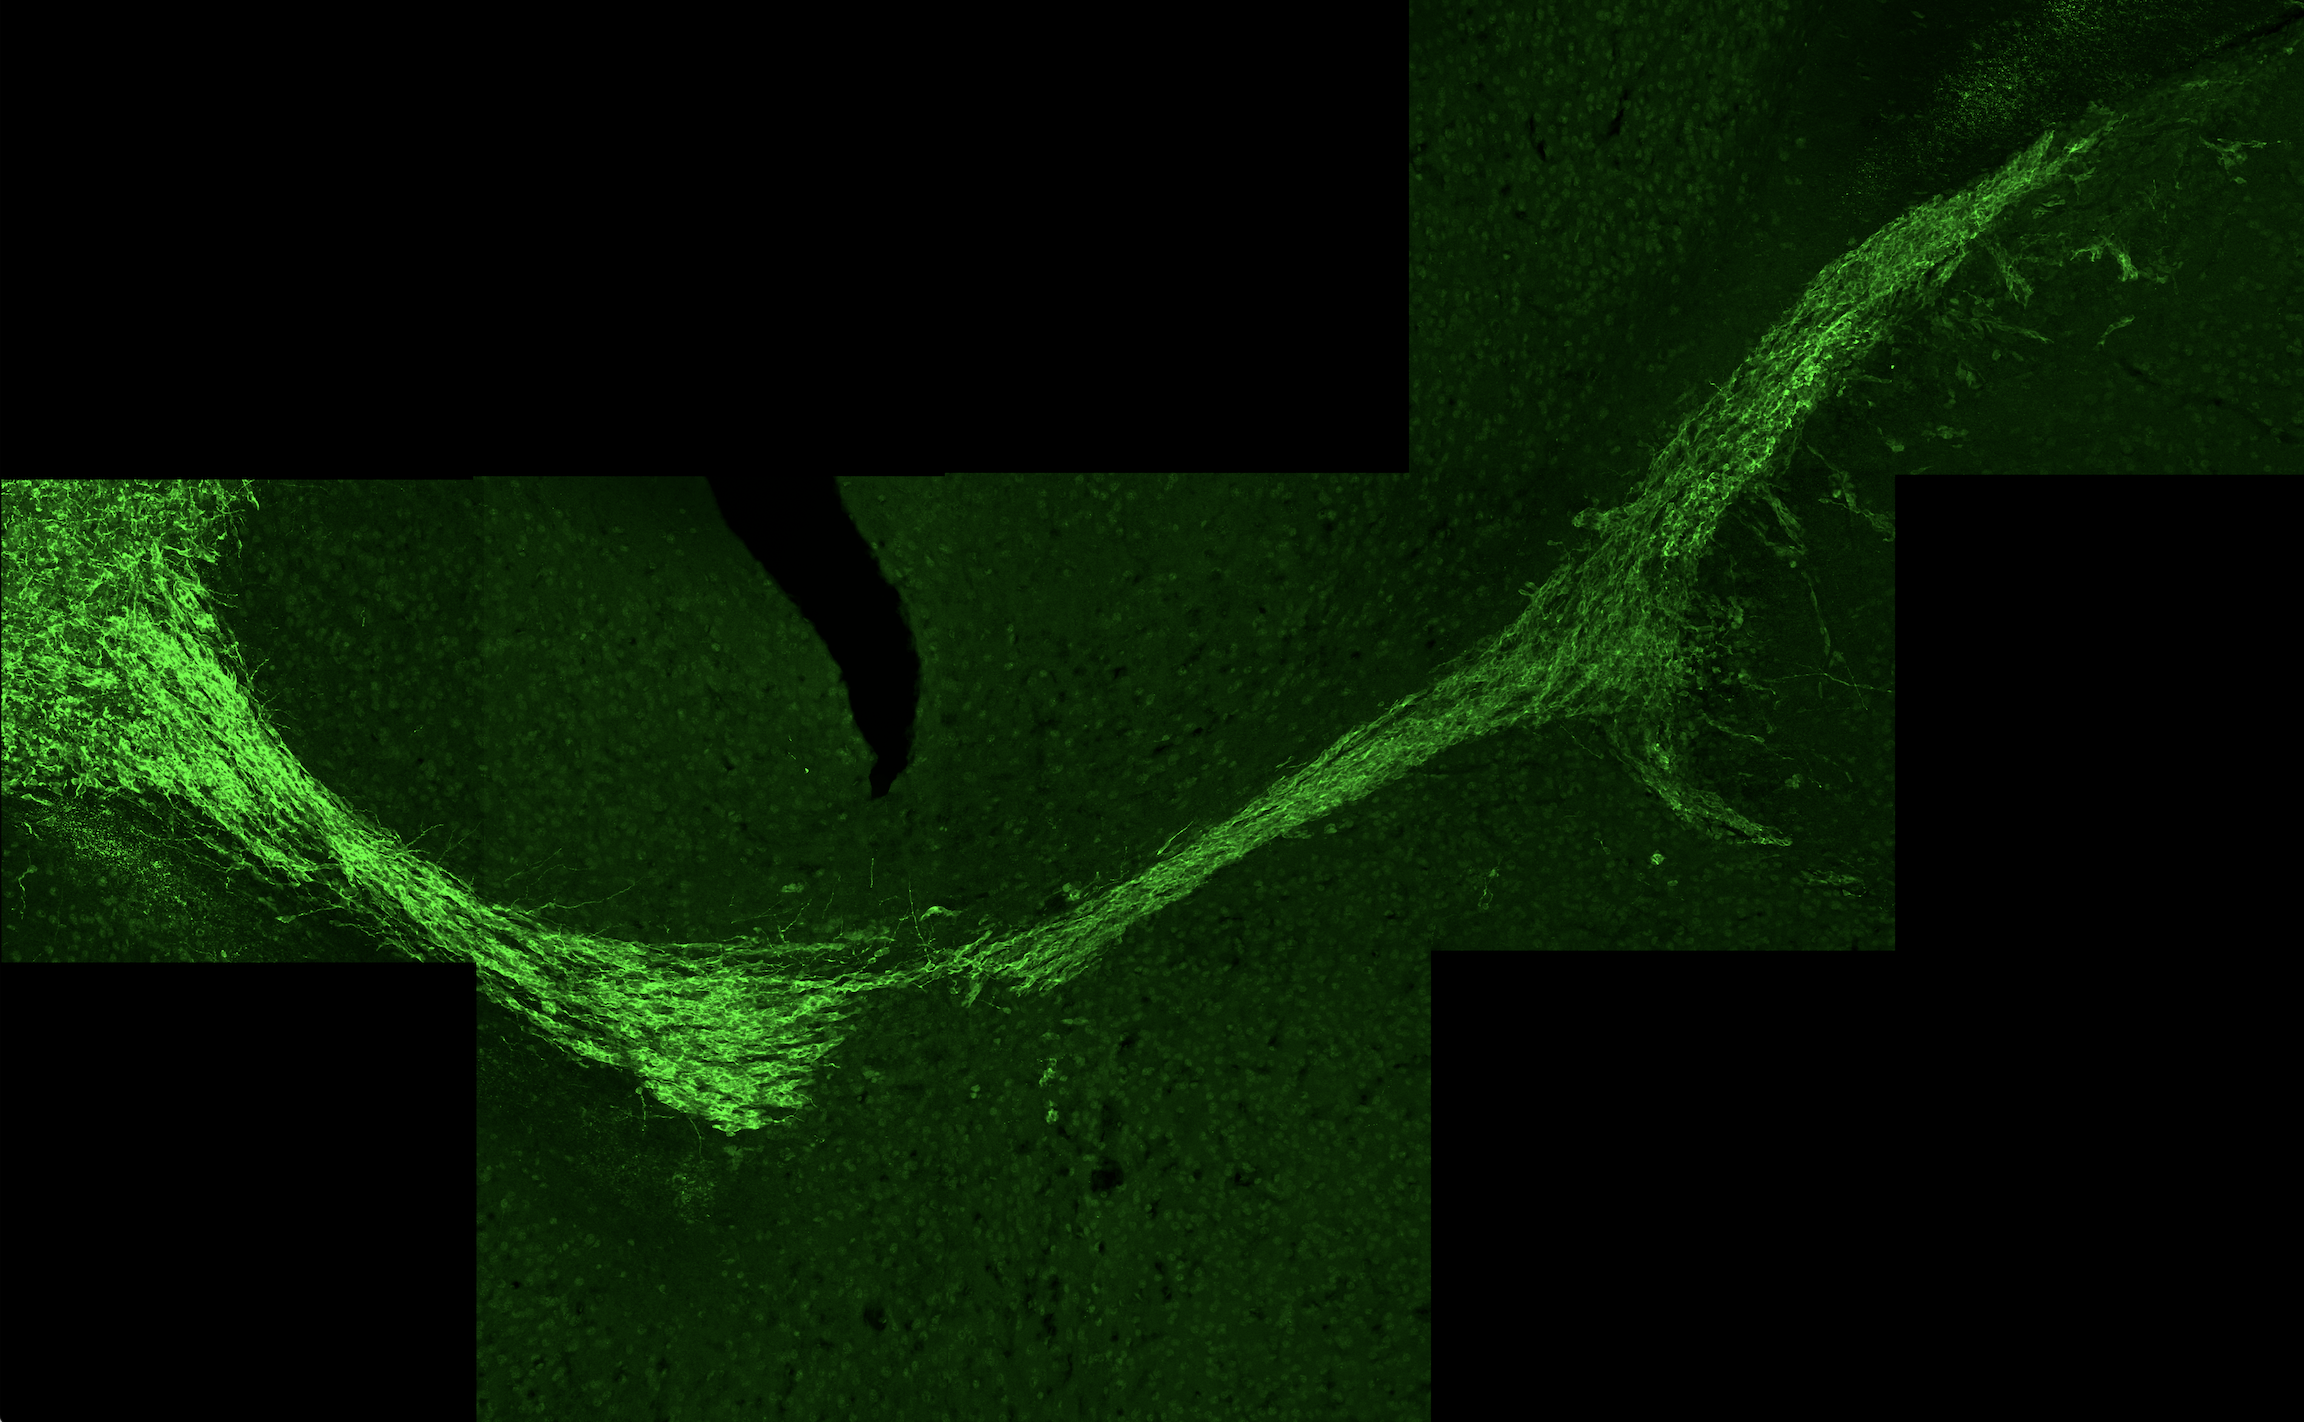
\includegraphics[width=0.95\linewidth]{via-verde}}
\end{frame}

\begin{frame}{Segundo objetivo: modelización y ajuste de parámetros}
	\begin{equation}
	\label{eq:neuroblast}
	\tau u_t + \X\, \nabla \cdot(u\nabla \O) + \alpha\, u - \gamma\, u \,1_{\NZdomain} 
	= \beta\, 1_{\SVZdomain}  
	\qquad\text{in}\enspace\Omega\times [0,T],
	\end{equation}
	\vspace{3mm}
	\begin{equation}
	\label{source}
	f_{\O}(x,y) = f_{\O}(\SO; x,y) 
	=  e^{((x-x_O)^2 + (y-y_O)^2)/\SO^2}.
	\end{equation}
	\vspace{3mm}
	\begin{equation} 
	\label{ob}
	\left\{ \begin{aligned} \Olf-\nabla\cdot (\mu_\CCdomain\,\nabla \Olf) &= f_{\O}  \quad  \text{ in } \Omega, \\
	\Olf &= f_{\O}  \quad \text{ on } \partial\Omega.
	\end{aligned}
	\right.
	\end{equation}
\end{frame}

\begin{frame}{Cerebro virtual}
	Malla
	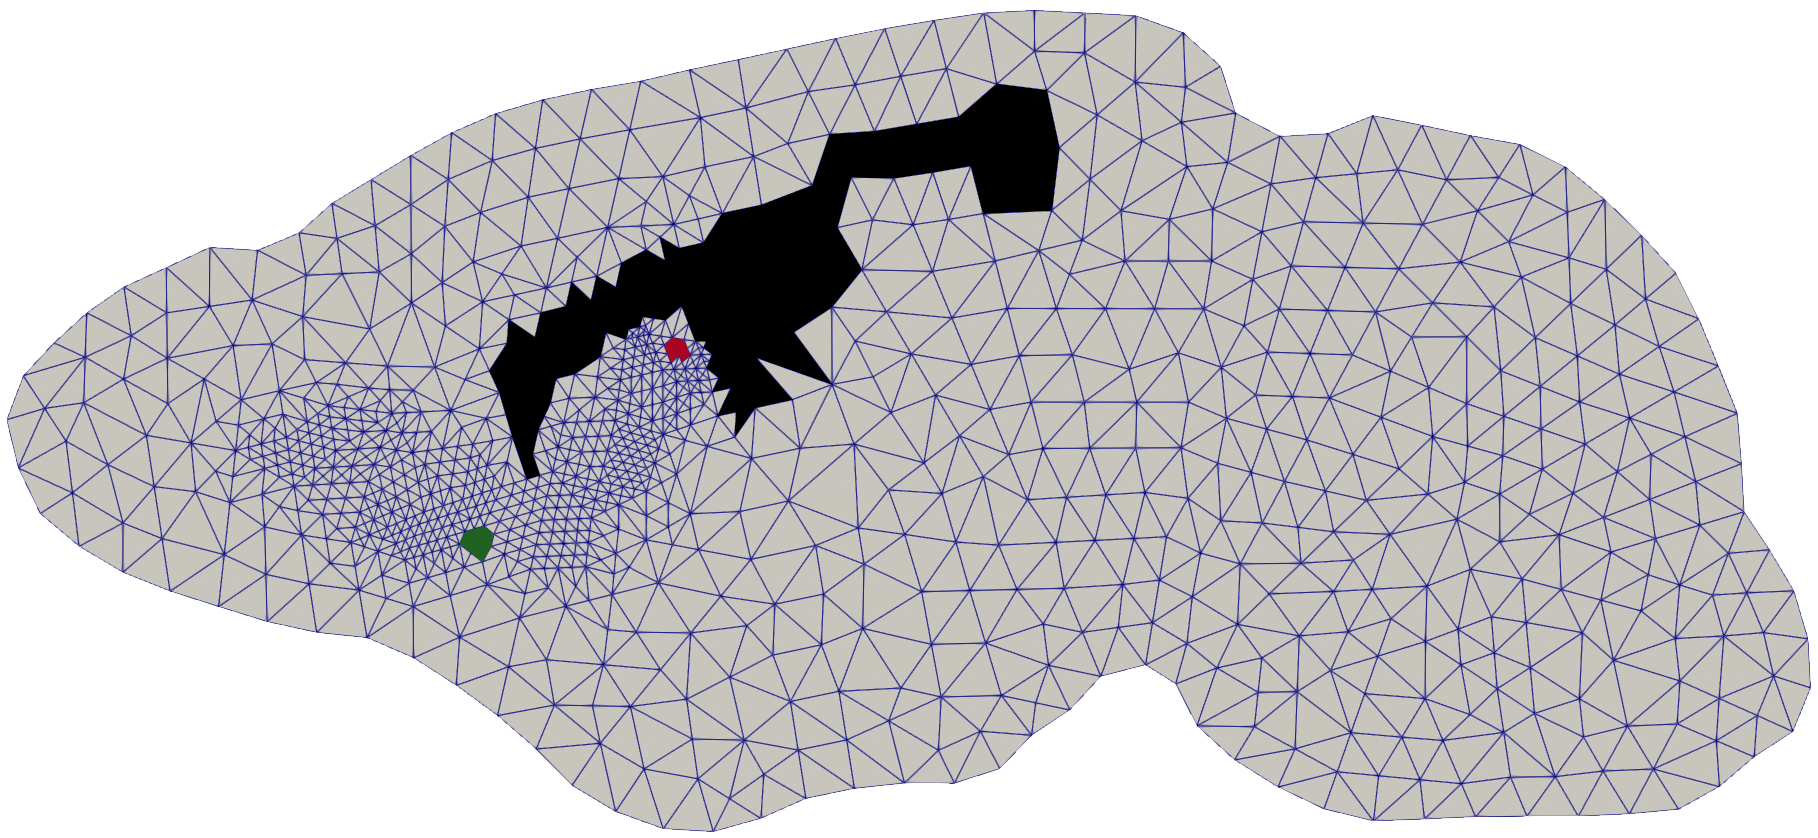
\includegraphics[width=0.95\linewidth]{brain-mesh.png}
\end{frame}

\begin{frame}{Modelización de la atracción}
Gradiente del bulbo olfatorio: parámetro $\sigma$
 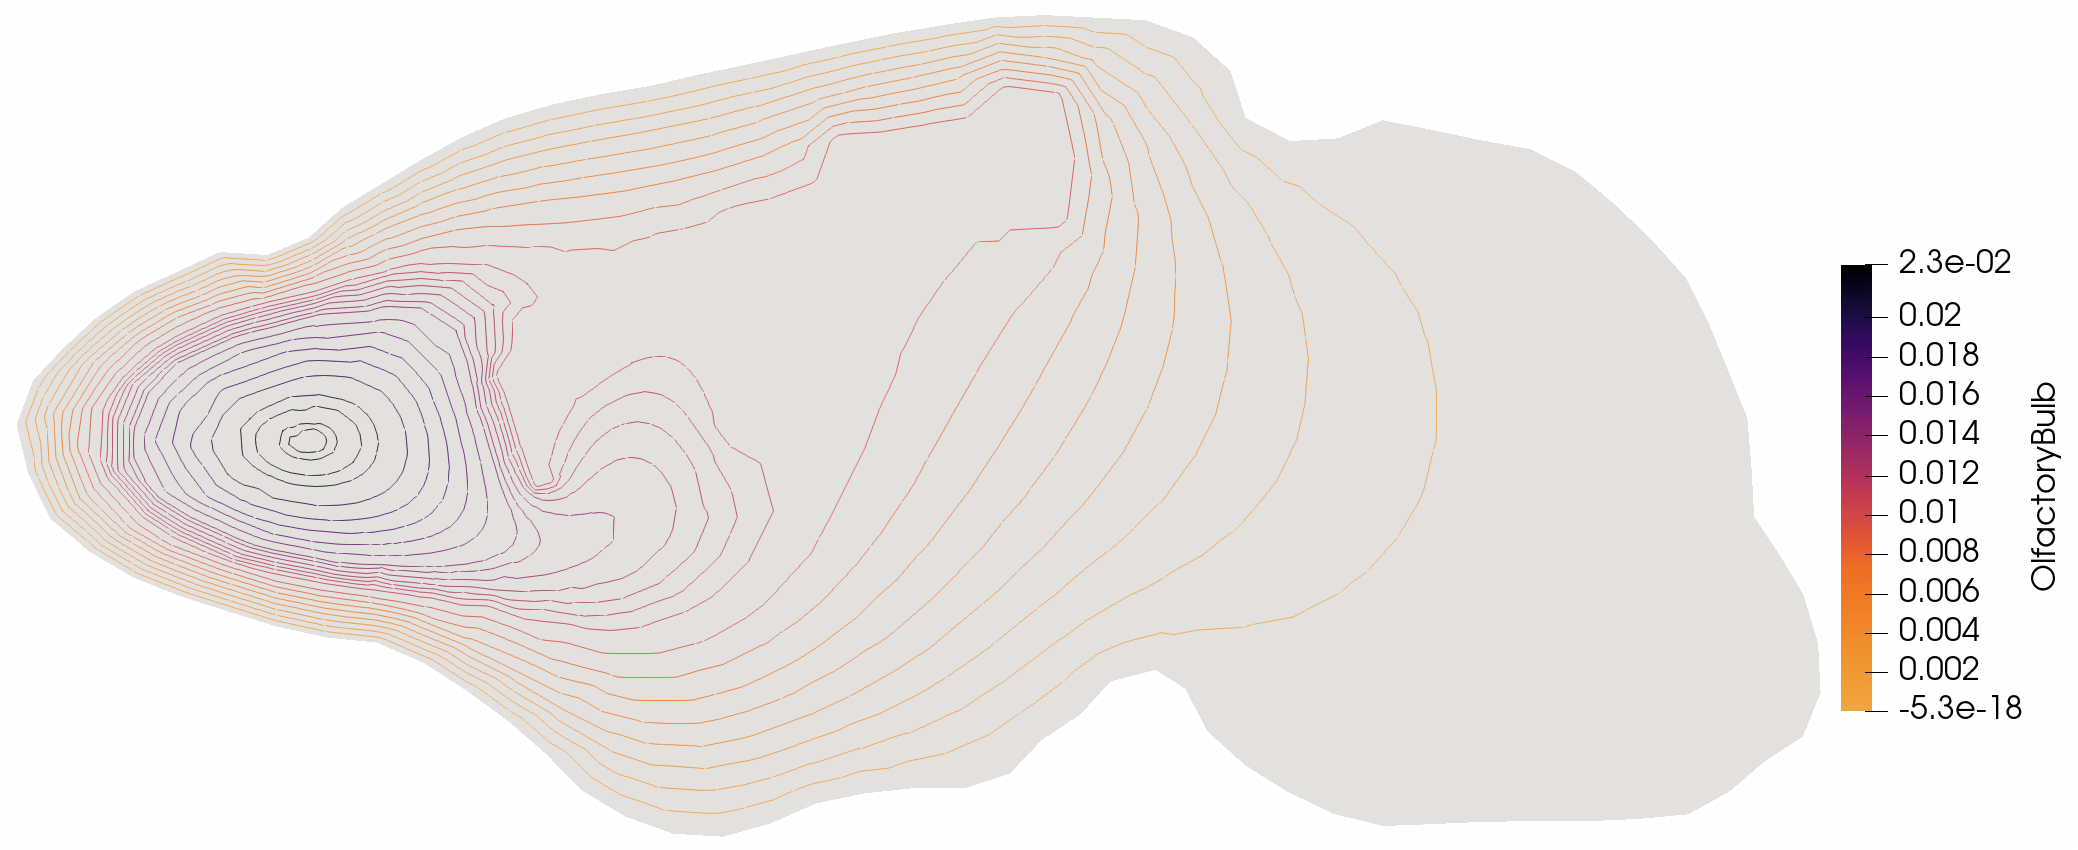
\includegraphics[width=0.95\linewidth]{ob.png}
\end{frame}
\begin{frame}{Modelización del movimiento}
	Vía rostral: parámetros $\alpha, \beta, \X, \gamma$
	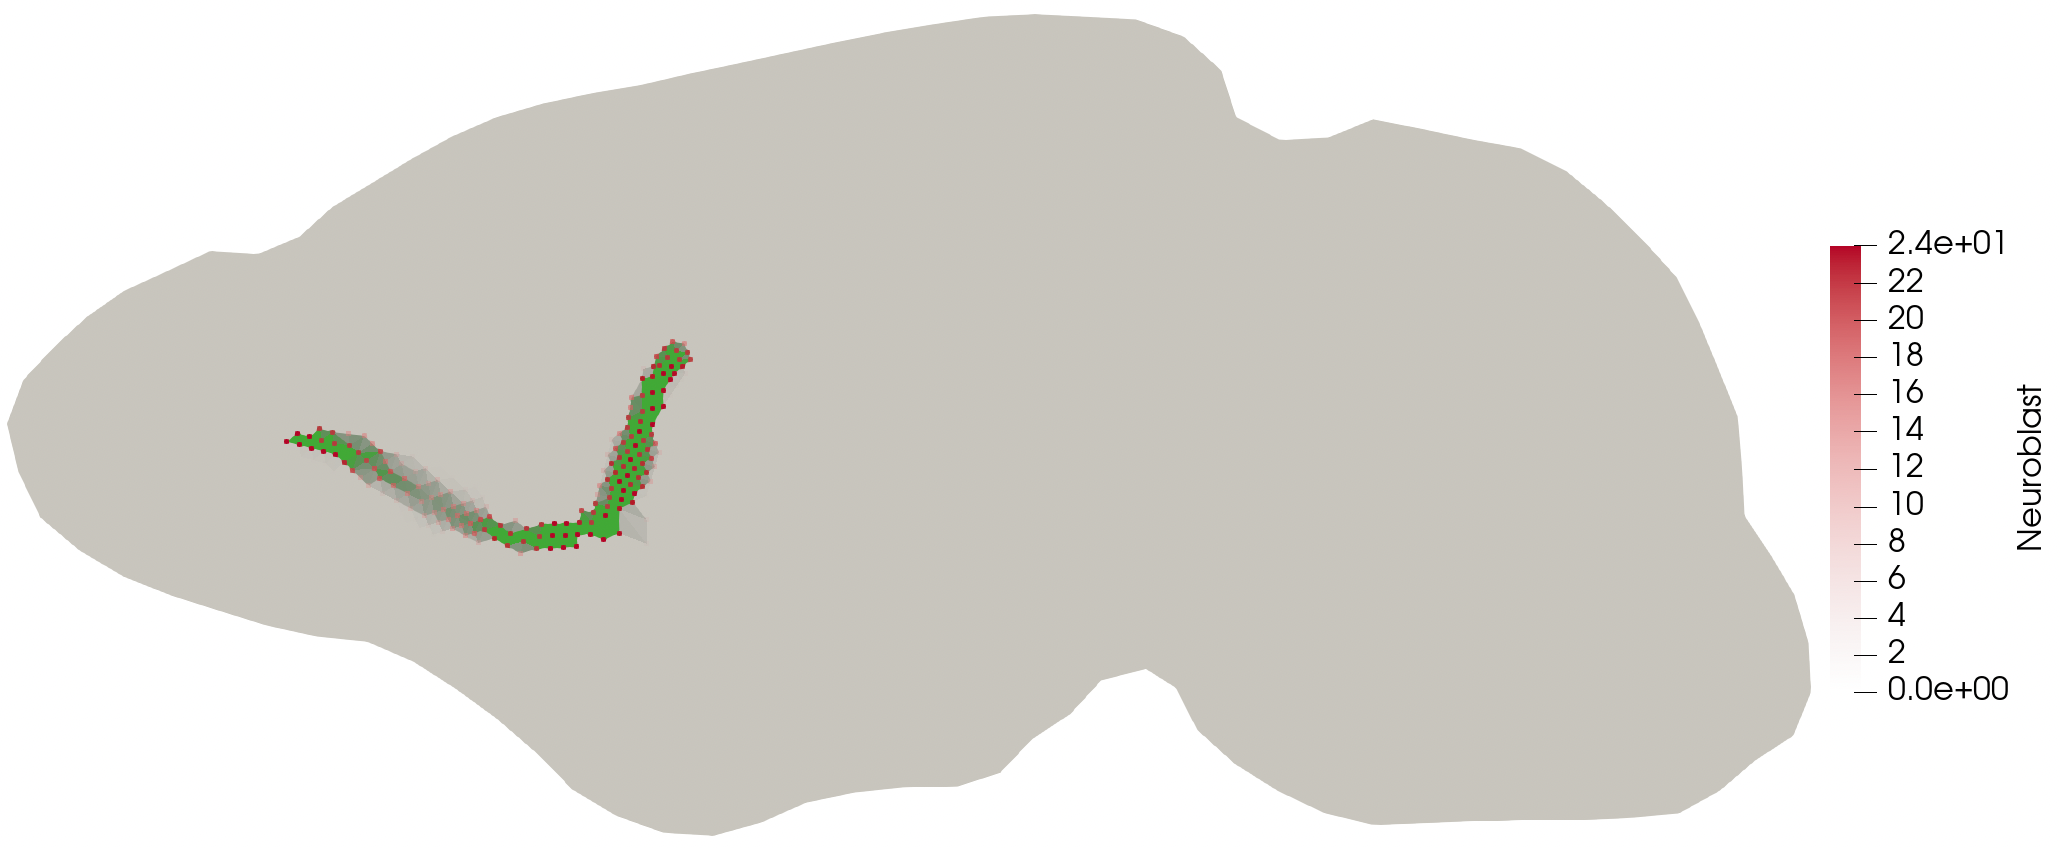
\includegraphics[width=0.95\linewidth]{steady-opt.png}
\end{frame}




%\include{dan1}
%\include{noelia}
%\include{dan2}


%\include{dan2}


%\include{dan2}


%\include{dan2}

